\documentclass[12pt,twoside]{report}
    \usepackage{amsmath}
    \usepackage{nccmath}
    \usepackage{amsfonts}
    \usepackage{lscape}
    \usepackage[utf8]{inputenc}
    \usepackage{titlepic}
    \usepackage{stackengine}
    \usepackage{lipsum}
    \usepackage{enumitem}
    \usepackage[toc,title,page]{appendix}
    \linespread{1.18} 
    \usepackage[]{graphicx}
    \usepackage[section]{placeins}
    \usepackage{booktabs}
    \usepackage{cite}
	\usepackage{float}
	\usepackage{caption}
	\usepackage{adjustbox}
    \usepackage{subcaption}
    \usepackage{multirow}
    \usepackage[a4paper,width=150mm,top=25mm,bottom=25mm]{geometry}
    \usepackage{fancyhdr}
    \usepackage{relsize}
    \usepackage{titlesec}
    \titleformat*{\section}{\large\bfseries}
	\titleformat*{\subsection}{\large\bfseries}
	\titleformat*{\subsubsection}{\normalsize\bfseries}
    \usepackage{tikz}
    \usetikzlibrary{shapes.geometric,arrows}
	\makeatletter
    \setlength{\@fptop}{0pt}
    \makeatother
    \tikzstyle{startstop} = [rectangle, rounded corners, minimum width = 4cm, minimum height=1cm, text centered,text width = 5cm, draw = black, fill=white!10]    
     \tikzstyle{process} = [rectangle,  minimum width = 5cm, minimum height=1.5cm, text centered, text width = 5cm,draw = black, fill = white!10]  
	 \tikzstyle{decision} = [diamond, minimum width = 4cm, minimum height=1cm, text centered,text width = 3cm, draw = black, fill = white!10]  
     \tikzstyle{arrow} = [thick,->,>=stealth]  


\usepackage{titling}
\pretitle{\begin{center}\fontsize{18bp}{18bp}\selectfont}
    \posttitle{\vspace{25bp}\par
\includegraphics[width=60mm]{logo.png}\par\end{center}}
\preauthor{\begin{center}\fontsize{14bp}{14bp}\selectfont}
    \postauthor{\par\end{center}}
\predate{\begin{center}}
    \postdate{\par\end{center}}  

\title{\LARGE{\textbf{Development and implementation of material subroutines for fibre reinforced plastics in a commercial FEM software}}\\[0.7cm]\smaller \textbf{Master thesis \\[0.5cm] Winter semester 2018/19}\vspace*{1cm}}


\author{
\vspace{2cm}
\large{Presented by: Arun prakash Ganapathy}
\\[0.4cm]
\large{Supervised by: Dr.-Ing Dominik Laveuve}
\\[0.4cm]
\large{Mat.Nr: 63876}
\\[0.4cm]
\large{E-mail: arun-prakash.ganapathy@student.tu-freiberg.de}}
\date{}

\newcounter{savepage}
\begin{document}
\pagenumbering{Roman}
\maketitle
\newpage
\tableofcontents
 \listoffigures
 \listoftables
 
\newpage
\setcounter{savepage}{\arabic{page}}
\pagenumbering{arabic}
\chapter{Introduction}
\section{Background and motivation}
\indent\indent\indent Composite materials are made of two or more dissimilar materials of different physical or chemical properties, which, when combined, create a material with properties unlike the individual constituent materials. One of the earliest use of composite materials date back to 3400 B.C when Mesopotamians glued wood strips at different angles to create plywood. Now a days advanced composite materials are widely used in structural design in various industries such as aerospace, automobile, marine, petrochemical etc., due to their superior properties over traditional engineering materials.\\
\begin{figure}[htbp]
\begin{center}
\includegraphics[width=1\textwidth]{{composite plane.jpg}}
 \caption{Composite materials used in a Boeing 787 'Dreamliner'}
 \label{fig:Composite plane}
\end{center}
\end{figure}
\FloatBarrier
\indent\indent\indent Composite materials are attractive because of their high strength, high stiffness-to-density ratio, light weight properties etc., Another important reason for using composite materials is the ability to tailor the stiffness and strength to specific design loads flexibly. Despite their superior physical properties, composite materials can be damaged from a number of sources, both during initial processing and in operation. Since composite materials have complex material response and a negligible margin of safety through ductility as offered by metals, the development of damage must be understood for predicting failure of such materials. For example fibre-reinforced plastics exhibit local damage such as fibre breakage, matrix cracks, fibre matrix debonds etc., under normal operating conditions which may contribute to the failure. Therefore the ability to predict the initiation and growth of damage is important for predicting the performance, safety and reliability of the composite materials for commercial use.\\
\indent\indent\indent Several methods have been proposed to analyze the failure of composite materials. The simplest of them is to degrade the stiffness of the material instantaneously using a degradation factor once the failure criteria is met. While easy to implement, the sudden complete failure of the material does not agree well with the real-life behaviour. Progressive failure analysis of composite materials is required to predict the real-life mechanical behaviour under various loading conditions.  Over the last few decades continuum damage mechanics (CDM) first proposed by Kachanov (1987), has been employed to analyse the progressive degradation of the materials. The CDM approach provides a methodology which can determine the full range of deterioration of the material starting from no damage to the fully disintegrated material. 
\begin{figure}[htbp]
\begin{center}
\includegraphics[width=0.65\textwidth]{{strain-softening.png}}
 \caption{Strain-softening of composite materials after damage initiation}
 \label{fig:Strain-softening}
\end{center}
\end{figure}
\FloatBarrier
In CDM the damage is  represented by a set of damage variables which describes the current state of the material, and their development using set of evolution laws. Once the failure criteria is met, the damage variables are calculated using these evolution laws and the stiffness of the material is degraded with the help of the damage variables i.e., the material experiences strain-softening rather than strain-hardening observed in metals Figure (\ref{fig:Strain-softening}).  The very fact that the damage can be represented as  a set of variables, makes them suitable for numerical simulations. Damage formulations can be easily fitted into non-linear finite element (FE) algorithms with the help of constitutive relations and implemented in simulation codes without the need to rely on special discretization techniques.

\section{Scope and Outline}
\indent\indent\indent  The objective of the thesis is to develop progressive damage models for predicting the initiation and propagation of damage in an orthotropic material when subjected to various loading conditions. Continuum damage mechanics (CDM) provides the framework for developing these damage models. Since the orthotropic materials exhibit different material properties in mutually perpendicular directions, the model essentially consists of linear elasticity extended with an anisotropic damage mechanism. Therefore one damage variable is assigned to each principal material direction to represent the development of damage i.e., 2 damage variables are required when the problem is in 2D/Plane-stress  and 3 variables when the problem is in 3D. The numerical modelling of the strain-softening behaviour results in strong mesh dependency which results in convergence issues when the mesh is refined. To reduce the mesh sensitivity, the fracture energy approach is used which includes fracture energy in the damage evolution laws. This ensures the objectivity of the model by adjusting the energy dissipated by each failure mechanism using a characteristic element length.\\
The stages of the thesis work are briefly described as follows\\\\
\textbf{Chapter 2} introduces the theoretical framework of continuum damage mechanics (CDM), constitutive relations and constitutive equations necessary for developing orthotropic material model. \\\\
\textbf{Chapter 3} gives reader a brief introduction into software used and the instructions to develop, compile and implement a material model in an FE environment. \\\\
\textbf{Chapter 4} gives a brief introduction to the mechanisms of damage and the different types of failure criteria and evolution equations necessary for developing damage models. In the end, the chapter deals with regularization method used to reduce mesh sensitivity problems and a brief description of how to implement the damage models step by step in a programming software. \\\\
\textbf{Chapter 5} The results of the finite element simulations are discussed in this chapter. Starting with the implementation of linear elastic behaviour of the orthotropic material the chapter discusses the behaviour of the damage models at integration point level and using representative structural examples.  

\newpage
\vspace*{15cm}
\chapter{Continuum damage mechanics}
\indent\indent\indent Continuum damage mechanics (CDM) is a theory for analyzing damage and fracture processes in materials from a continuum mechanics point of view. (CDM) provides a continuum perspective for microflaws initiation, propagation, and their coalescence that eventually results in macroscopic faults and fractures. CDM uses state variables to represent the damage effect on the stiffness and remaining life of the material that is deteriorating as a result of load and ageing. A damage activation function is required to predict the initiation of damage. Damage evolution does not progress spontaneously after initiation therefore, a mathematical model is required.  

\section{Damage}
\indent\indent\indent  Consider a body B of Fig. \ref{fig:Damage}  where a crack of length $a$ has developed due to an external load F.  If we take an arbitrary point P($x$) near the crack tip, a number of microscopic cavities or microcracks would be observed around the region.
These cavities are usually developed due to breakage of atomic bonds, or some defects in the atomic array. From the microscopic point of view, fracture of materials is a process of nucleation of microcavities or microcracks due to the breakage of atomic bonds. From the macroscopic point of view, it is a process of extension of cracks brought about by the coalescence of these microcracks.\\
\indent\indent\indent From the mesoscopic point of view, which exists between microscopic and macroscopic scale, it is a process of nucleation, growth and the coalescence of microscopic cavities that leads to the initiation of macroscopic crack. The development of microscopic, mesoscopic and macroscopic processes of fracture in materials and the resulting deterioration in their mechanical properties is called damage. Continuum damage mechanics aims to analyse the damage development during mesoscopic and macroscopic fracture processes in the framework of continuum mechanics.
\begin{figure}[htbp]
\begin{center}
\includegraphics[width=0.5\textwidth]{{1. Damage.png}}
 \caption{Scales of damage observation}
 \label{fig:Damage}
\end{center}
\end{figure}
\FloatBarrier

\section{Representative Volume Element(RVE)}
\indent\indent\indent  To discuss the effects of microscopic discontinuities in a material using CDM we must homogenize the mechanical effects of microstructure and represent them as a macroscopic continuous field in the material. For this purpose, we take a small region of a mesoscale around the material point P($x$) in body B, as shown in Figure. \ref{fig:Damage}. We assume that the material with discontinuous structures in this region as homogeneous, and the mechanical state of the material in this region can be represented by the statistical average of the mechanical variables in that region. This region is said to be the Representative Volume Element(RVE). For such RVE, the following two conditions must be satisfied:
\begin{itemize}
\item  For the material in the RVE to be statistically homogeneous, the RVE should be large enough to contain a sufficient number of discontinuities
\item To represent a non-uniform macroscopic mechanical field by means of a continuum, the size of RVE should be sufficiently small so that the variation of the macroscopic variable in it may be insignificantly small
\end{itemize}
The size of RVE depends on the microstructure of the relevant material and their typical sizes are as follows
\begin{itemize}
\item Metals and ceramics  \;    -    \; 0.1\;$mm^3$
\item Polymers and composites \;   -   \; 1\;$mm^3$
\item Timber\; - \; 10\;$mm^3$
\item Concrete \; - \; 100\;$mm^3$
\end{itemize}

\section{Concept of continuum damage mechanics (CDM)}
\indent\indent\indent The basic concept of CDM is that a set of damage variables can represent the microstructural defects in a material. Continuum damage mechanics first represent the damage state of a material in terms of a set of internal state variables and then describe the mechanical behaviour of the damaged material and then development of damage by use of these state variables. The mechanical behaviour of a damaged material can be described using the notion of effective stress, together with the hypothesis of mechanical equivalence between damaged and undamaged material. The concept of effective stress and mechanical equivalence will be discussed in the following sections.
\subsection{Modelling by Effective area reduction}
Let us consider body B of Fig. (\ref{fig:Damage2}) and take an RVE at an arbitrary point $P(x)$ in B. If the total void area in $dA$ is  $ dA_{D} $, the mechanical effect of $dA$ will be decreased by $dA_{D}$. Then the area,
\begin{equation}
  d\tilde{A} = dA  - dA_{D}
  \label{eqn:da} 
\end{equation}
may be interpreted as the area which carries the internal force and is called an $effective$ $area$. Thus, the damage variable D can be specified as 
\begin{equation}
 \label{eqn:D}
  D = \frac{dA - d\tilde{A}}{dA} = \frac{dA_{D}}{dA}
\end{equation}
where the damage variable D takes a value between 0 and 1 ($0 \leq D \leq 1$). $D = 0$ represents initial undamaged state and $D=1$ represents fully damaged state.
\begin{figure}[htbp]
\begin{center}
\includegraphics[width=0.8\textwidth]{{Damage2.png}}
 \caption{Effective area reduction due to microcracks}
 \label{fig:Damage2}
 \end{center}
\end{figure}
\FloatBarrier
Suppose a cylindrical bar of cross-sectional area $dA$ is subject to a tensile load $dF$, then the actual load carrying area is $ d\tilde{A}$ rather than $dA$. According to eqns (\ref{eqn:da}) and (\ref{eqn:D}) the effective area $ d\tilde{A}$ is given by,
\begin{equation}
\label{eqn:da_t}
 d\tilde{A} = (1-D)dA
\end{equation}
The decrease in the load-carrying area increases the effect of stress $\sigma$ induced by the external force $dF$. Due to eqn \ref{eqn:da_t}, the magnified stress $\tilde{\sigma}$ is given by,
\begin{equation}
\label{eqn:sig_t}
\tilde{\sigma} = \frac{dF}{d\tilde{A}} = \frac{\sigma}{1 - D}
\end{equation} 

Since the stress $\tilde{\sigma}$ represents the stress magnified by the net area reduction due to damage, it is called  $effective$ $stress$. From eqn (\ref{eqn:da_t}) and (\ref{eqn:sig_t}) we can postulate that the damaged cylindrical bar of Figure.(\ref{fig:Damage3}b) with the cross-sectional area $dA$ subject to force $dF$ is mechanically equivalent to the  fictitious  undamaged bar of Figure.(\ref{fig:Damage3}c), which is subject to force $dF$, has the cross-sectional area $ {d\tilde{A}} $ and hence stress $\tilde{\sigma}$  
\begin{figure}[htbp]
\begin{center}
\includegraphics[width=0.8\textwidth]{{3. Damage_cylinder.png}}
 \caption{Damage of bar under tensile load}
 \label{fig:Damage3}
 \end{center}
\end{figure}
\FloatBarrier

\subsection{Modelling by variation of elastic modulus} 
\indent\indent\indent Since the development of microcavities causes the reduction in material stiffness, the damage state can be characterized by variation in elastic modulus. Let us consider the bar (b) and (c) of Figure. (\ref{fig:Damage3}) are in the damaged and fictitious undamaged state, respectively. Then the elastic strain $\epsilon$ in the bar (c) caused by stress $\tilde{\sigma}$ should be equal to the $\epsilon$ of the bar (b) under stress $\sigma$; i.e.,\\
\begin{equation}
\label{eqn:sig_t2}
   \tilde{\sigma} = E_{0}\epsilon, \;\;  \sigma = E(D)\epsilon 
\end{equation}
\\
\begin{equation}
\label{eqn:epsilon}
\epsilon = \frac{\sigma}{E(D)} = \frac{\tilde{\sigma}}{E_{0}}
\end{equation}
where $E_{0}$ and $E(D)$ are the young's modulus of the material in the initial undamaged state and in damaged state after loading, respectively. Therefore, eqn. (\ref{eqn:epsilon}) defines another effective stress\\
\begin{equation}
\label{eqn:epsilon2}
  \tilde{\sigma} = \frac{E_{0}}{E(D)}\sigma
\end{equation}
By combining Eqn. (\ref{eqn:sig_t}) and (\ref{eqn:epsilon}) we get,
\begin{equation}
\label{eqn:E(d)}
E(D) = (1 - D) E_{0}
\end{equation}
\begin{equation}
\label{eqn:D2}
D  = 1 - \frac{E(D)}{E_{0}}
\end{equation}
Therefore, the damage variable $D$ is characterized by the variation in Young's modulus $E(D)$. The modelling of damage by means of reduction in stiffness can be applied also to the anisotropic damage of brittle materials like composite materials, concrete, rocks etc.,
\section{Mechanical representation of the damage state}
\indent\indent\indent The deformation of material depends on the direction of applied stress or strain, and hence it is an anisotropic phenomena. Therefore different theories have been developed for modelling 3-D anisotropic damage phenomenon. Some fundamental theories that describe 3-D damage state are given below. 
\subsection{Scalar damage variable}
\indent\indent\indent In the case of random or isotropic distribution of microcracks or voids, and when void density is small, the global mechanical properties can be approximated as nearly isotropic. The damage state, in this case, may be represented using scalar damage variable D. Thus isotropic damage theory based on isotropic damage variable has been often applied to 3-D problems of creep, elastic-plastic, ductile and fatigue damage
\subsection{Vector damage variable}
\indent\indent\indent The damage state can be specified by the decrease in load carrying effective area due to void development. Hence it is easy to postulate a vector damage variable. Kachanov (1974, 1986) tried to extend the definition of damage to anisotropic damage by noting a surface element in an arbitrary direction $n$, he proposed vector damage variable $ \omega = \omega_{n}n$, where $\omega_{n}$ is the effective area fraction. 
\subsection{Damage tensor of second order}
\indent\indent\indent To describe an anisotropic damage state, a damage variable of second or higher order tensor is required. Eqn.(\ref{eqn:da_t}) suggests that the damage state (1 - D) is specified by the transformation of the surface element $dA$ of Fig. (\ref{fig:Damage3}b) of the damage state into the corresponding surface element $d\tilde{A}$ in the fictitious undamaged state of Fig.(\ref{fig:Damage3}c). 
\begin{figure}[htbp]
\begin{center}
\includegraphics[width=0.5\textwidth]{{4. Damage.png}}
 \caption{Surface element in RVE of a damaged material}
 \label{fig:Damage4}
 \end{center}
\end{figure}
To express damage as a second order tensor, we first consider an arbitrary surface element $PQR$ in RVE in the current damaged configuration $B_{t}$ of Fig.(\ref{fig:Damage4}a). The unit normal vector and area of $PQR$ are denoted by $\nu$ and $dA$. We further postulate the fictitious undamaged configuration $B_{f}$ of Fig.(\ref{fig:Damage4}b) mechanically equivalent to $B_{t}$, and the surface element and its area vector are denoted by $\tilde{P}\tilde{Q}\tilde{R}$ and $\tilde{\nu}d\tilde{A}$ respectively. According to Eqn.(\ref{eqn:da_t}) the damage variable of second-order tensor $D$ should be defined by linear transformation from area vector $\nu dA$ in $B_{t}$ into $\tilde{\nu}d\tilde{A}$ in $B_{f}$, i.e.,
\begin{equation}
\label{eqn:second_order_tensor}
\tilde{\nu}d\tilde{A} = (I - D)\nu dA
\end{equation}
where $I$ is the second order identity tensor. Since the damage tensor $D$ is symmetric, it can be expressed by its spectral decomposition
\begin{equation}
\label{eqn:damage_2nd_order}
D = \sum_{i = 1}^{3} D_{i}n_{i}  \otimes D_{i}n_{i}
\end{equation}
where $D_{i}$ and $n_{i}$ are the principal values and principal directions of $D$. 

\section{Effective Stress Tensors}
\indent\indent\indent The effective stresses are used to describe the mechanical behaviour of the damaged material. Some of the effective stresses postulated in damage mechanics are given below
\subsection{Effective stress tensor for isotropic damage}
\indent\indent\indent If the damage state is isotropic then the effective stress tensor of three-dimensional state is given by
\begin{equation}
\tilde{\sigma} = (1 - D)^{-1} \; \sigma
\end{equation}
where D is the scalar damage variable, and $\sigma$ is the Cauchy stress tensor. This effective stress simplifies damage theory and can be applied to a number of damage problems like ductile damage. But this cannot be applied to damage of significant anisotropy, such as brittle damage due to microcrack distribution.\\
\subsection{Asymmetric effective stress tensor for anisotropic damage}
\indent\indent\indent The increase in stress caused by the net area reduction in case of anisotropic damage is given by
\begin{equation}
\tilde{\sigma} = (I - D)^{-1} \; \sigma
\end{equation}
where I and D are second-order identity tensor and the second-order damage tensor, respectively. In the actual development of anisotropic damage, the stress-induced in the RVE of damage material is asymmetric. But asymmetric stress tensors make the numerical analysis complicated, and thus different methods of symmetrization have been proposed. A few of them are described as follows

\subsection{Symmetrized effective stress tensor for anisotropic damage (Murakami and Ohno 1981)} 
\indent\indent\indent A simple symmetrization procedure of Eq.(\ref{eqn: Murakami and Ohno}), the symmetric part of the Cartesian decomposition of Eq.(\ref{eqn: Murakami and Ohno}) gives,
\begin{equation}
\label{eqn: Murakami and Ohno}
\tilde{\sigma} = \frac{1}{2} [(I - D)^{-1}\;\sigma + \sigma(I - D)^{-1}]
\end{equation}\\


\section{Damage effect tensors}\label{Matrix Representation of Damage effect tensors}
\indent\indent\indent The general form of an effective stress tensor $\tilde{\sigma}$ is given by the damage effect tensor $\mathbb{M}$ and the corresponding Cauchy stress tensor $\sigma$, i.e.,
\begin{equation}
\tilde{\sigma}  = \mathbb{M} \; :  \sigma 
\label{eqn:effective_stress_tensor} 
\end{equation}
It is convenient to express the tensors in the form of matrices and then execute the tensor operations as a matrix calculus.. To simplify this procedure, we take an orthonormal basis ${n_{i}}$ with principal directions $n_{i}$ of the second-order symmetric damage tensor $D$, and represent the tensor in terms of its component to this basis. According to Voigt notation, the second-order symmetric tensor $\sigma$ and the related effective stress $\tilde{\sigma}$ are expressed by the column vector of six dimensions:
\begin{equation}
   [\sigma_{P}]  \equiv  [\sigma_{11} \;\; \sigma_{22} \;\;\sigma_{33} \;\;\sigma_{12} \;\;\sigma_{13} \;\;\sigma_{23} ]^{T}
\end{equation}

\begin{equation}
   [\tilde{\sigma_{P}}]  \equiv  [\tilde{\sigma_{11}} \;\; \tilde{\sigma_{22}} \;\;\tilde{\sigma_{33}} \;\;\tilde{\sigma_{12}} \;\;\tilde{\sigma_{13}} \;\;\tilde{\sigma_{23}} ]^{T}
\end{equation}
\\
By means of the matrix representation, we have the matrix form
\begin{equation}
[\tilde{\sigma_{P}}] \equiv [\mathbb{M}_{pq}]\;: [\sigma_{P}]
\label{eqn:Matrix_rep_damage_effect_tensor}
\end{equation}
\\
Matrix representation of the damage effect tensor of Eq.(\ref{eqn:Matrix_rep_damage_effect_tensor}) is shown below
\\
$$
[\mathbb{M}_{pq}] \equiv   
 \begin{bmatrix}
   \frac{1}{\omega_{11}}  \; & 0 \; & 0 \; & 0 \; & 0\; & 0 \\
  \\
  0\; & \frac{1}{\omega_{22}}\; & 0\; & 0\; & 0\; & 0 \\
  \\
  0\; & 0 \; & \frac{1}{\omega_{33}}\; & 0\; & 0\; & 0 \\
  \\
  0\; & 0\; & 0\; & \frac{1}{\omega_{12}}\; & 0\; & 0 \\
  \\
  0\; & 0\; & 0\; & 0\; & \frac{1}{\omega_{23}}\; & 0 \\
  \\
  0\; & 0\; & 0\; & 0\; & 0\; & \frac{1}{\omega_{13}}  
  \\
 \end{bmatrix}
 \label{Damage_effect_tensor}
 $$
\\
where
$$\omega_{11} \; = \; (1 - d_{1}) \;\;  \omega_{22} \; = \; (1 - d_{2}) \;\; \omega_{33} \; = \; (1 - d_{3})$$ \vspace*{0.1cm} $$\omega_{12} \; = \; \sqrt{(1 - d_{1})(1 - d_{2})}  \;\;\omega_{23} \; = \; \sqrt{(1 - d_{2})(1 - d_{3})} \;\; \omega_{13} \; = \; \sqrt{(1 - d_{1})(1 - d_{3})}$$

\section{Hypothesis of strain Equivalence}\label{Hypothesis of Strain Equivalence}

\indent\indent\indent The inelastic constitutive equation of a damaged material is given by the corresponding constitutive equation for an undamaged material by replacing the stress tensor $\sigma$ in the equation with the corresponding effective stress tensor $\tilde{\sigma}$. In Figure (\ref{fig:Strain_eq}). the effect of stress $\sigma$ acting on RVE in the current damaged configuration $B_{t}$ is equivalent to that of the stress $\tilde{\sigma}$ in the fictitious undamaged configuration. Therefore the deformation of the damaged material subject to stress $\sigma$ should be equal to that of the fictitious undamaged material subject to stress $\tilde{\sigma}$. Suppose the constitutive equation of an undamaged inelastic material is given by
\begin{equation}
  \epsilon = F_{0}(\sigma, \alpha)
\end{equation} 
or
\begin{equation}
  \dot{\epsilon} = F_{0}(\sigma, \alpha)
\end{equation}

where $\alpha$ is an internal variable representing the internal change other than damage. and ($\dot{}$) denotes the material time derivative
\begin{figure}[htbp]
\begin{center}
\includegraphics[width=0.8\textwidth]{{6. Strain_eq.png}}
 \caption{Hypothesis of strain equivalence}
 \label{fig:Strain_eq}
 \end{center}
\end{figure}
Then according to hypothesis of strain equivalence, the inelastic constitutive equation of the damaged material represented by a damage variable $D$ should be given by replacing $\sigma$ of Eq.(25) with the effective stress $\tilde{\sigma}$ i.e.,

\begin{equation}
    	\epsilon = F(\sigma, D, \alpha)  = F_{0}(\tilde{\sigma}, \alpha)
\end{equation}

or 
\begin{equation}
    	\dot{\epsilon} = F(\sigma, D, \alpha)  = F_{0}(\tilde{\sigma}, \alpha)
\end{equation}

In case of elastic deformation, constitutive equations for an undamaged and damaged material are given by
\begin{equation}
\epsilon = \mathbb{S}_{0}\; : \sigma,
\end{equation}\\
\begin{equation}
\epsilon = \mathbb{S}(D)\; : \sigma,
\end{equation}
where $\mathbb{S}_{0}$ and $\mathbb{S}(D)$  are fourth-order elastic compliance tensors of the materials. Therefore, according to the hypothesis of strain equivalence the elastic constitutive equation of the damaged material and the compliance tensor are given by 
\begin{equation}
\epsilon = \mathbb{S}_{0}\; : \tilde{\sigma}  =  [\mathbb{S}_{0}\;: \mathbb{M} (D)]\;: \sigma = \mathbb{S}(D)\; : \sigma
\end{equation}
\begin{equation}
\mathbb{S}(D) = \mathbb{S}_{0}\; : \mathbb{M} (D)
 \label{eqn:S_HSeq}
\end{equation}
where $\mathbb{M} (D)$ is the damage effect tensor which is given by 
\begin{equation}
\mathbb{M} (D)  = \mathbb{S}_{0}^{-1} \; : \mathbb{S}(D) 
\end{equation}

\section{Hypothesis of strain energy equivalence}\label{Hypothesis of strain energy equivalence}
\indent\indent\indent The existence of a strain energy function necessitates the symmetry of the compliance and elastic modulus tensor. But the compliance tensor resulting from the hypothesis of strain equivalence is asymmetric which does not satisfy the requirement. Therefore the hypothesis of strain energy equivalence is used to satisfy the symmetry requirements. Let us consider an elastic-plastic material and represent the internal change due to plastic deformation by an internal state variable $\alpha$. The complementary strain energy functions of the material at undamaged and damaged state are given, respectively as follows
\\
\begin{equation}
V_{0}(\sigma,\alpha) = \frac{1}{2}\sigma : \mathbb{S}_{0} : \sigma \; - \; \phi(\alpha)
\end{equation}
\\
\begin{equation}
V(\sigma,D,\alpha) = \frac{1}{2}\sigma : \mathbb{S}(D) : \sigma \; - \; \phi(\alpha)
\end{equation}
\\
Thus the constitutive equation for the undamaged and damaged material is 
\\
\begin{equation}
\epsilon = \frac{\partial V_{0} }{\partial \sigma} = \mathbb{S}_{0} : \sigma
\end{equation}
\\
\begin{equation}
\epsilon = \frac{\partial V }{\partial \sigma} = \mathbb{S}(D) : \sigma
\label{eqn:Strain_energy_eq}
\end{equation}

\begin{figure}[htbp]
\begin{center}
\includegraphics[width=0.8\textwidth]{{7.Strain_energy_eq.png}}
 \caption{Hypothesis of strain energy equivalence}
 \label{fig:Strain_energy_eq}
 \end{center}
\end{figure}
Suppose a damaged material of Figure.(\ref{fig:Strain_energy_eq})a subject to stress $\sigma$, and represent the damage and internal state due to inelastic deformation by $D$ and $\alpha$, respectively. Then the strain energy function $V(\sigma,D,\alpha)$ of the damaged material is given by replacing $\sigma$ in the corresponding function $V_{0}(\sigma,\alpha)$ of the undamaged material of Fig.(\ref{fig:Strain_energy_eq})b with the effective stress $\tilde{\sigma}$
\\
\begin{equation*}
V(\sigma,D,\alpha) \; = \; V_{0}(\tilde{\sigma},\alpha)
\end{equation*}
\\
By the use of this hypothesis, the elastic strain of Eq.(\ref{eqn:Strain_energy_eq}) leads to
\\
\begin{equation*}
\epsilon \; = \; \frac{\partial V(\sigma,D,\alpha)}{\partial \sigma} = \mathbb{S}(D) : \sigma 
\end{equation*}
\\
\begin{equation*}
\;\;\;\;\;\;\;\;\;\; = \; \frac{\partial V_{0}(\tilde{\sigma},\alpha)}{\partial \sigma} = \frac{\partial}{\partial \sigma}(\frac{1}{2}\tilde{\sigma} : \mathbb{S}_{0} : \tilde{\sigma} )
\end{equation*}
\\
\begin{equation*}
\;\;\;\;\;\;\;\;\;\;\;\;\;\;\;\;\;\; = \; \frac{1}{2}\frac{\partial}{\partial \sigma} [(\mathbb{M}(D):\sigma) : \mathbb{S}_{0} : (\mathbb{M}(D):\sigma)]
\end{equation*}
\\
\begin{equation}
= \;[\mathbb{M}^{T}(D) : \mathbb{S}_{0} : \mathbb{M}(D)]
\label{M_eqn}
\end{equation}
\\
From Eq.(\ref{M_eqn}), the elastic compliance tensor of the damaged material is given as follows
\\
\begin{equation}
\mathbb{S}(D) \; = \; \mathbb{M}^{T}(D) : \mathbb{S}_{0} : \mathbb{M}(D)
\label{eqn: S_HSEeq}
\end{equation}
\indent\indent\indent If the damage effect tensor $\mathbb{M}(D)$ can be expressed as a fourth-order symmetric tensor, then the elastic compliance tensor $\mathbb{S}(D)$ becomes a fourth-order symmetric tensor which satisfies the thermodynamic requirement. 

\section{Elastic constitutive equation and elastic modulus tensor of orthotropic material}\label{Constitutive matrix}
\indent\indent\indent Orthotropic materials are materials that exhibit different material properties along three mutually orthogonal axes. They are a special form of anisotropic materials because their properties change when measured from different directions. Some examples of orthotropic materials are wood, composite materials etc., Orthotropic materials require 9 independent variables to express their constitutive matrix. The 9 elastic constants are three Young's moduli $E_{x},E_{y},E_{z}$, the three Poisson's ratios $\nu_{xy},\nu_{yz},\nu_{zx}$, and three shear moduli $G_{xy},G_{yz},G_{zx}$. The elastic stiffness matrix of orthotropic material has the form,

\begin{equation}
  \sigma = \mathbb{C}_{0} : \epsilon \;\;\;   or \;\;\;  \sigma_{ij}  =  C^{0}_{ijkl}\epsilon_{kl},
\end{equation}

$$
\mathlarger{ [C^{0}_{pq}]} =  
 \begin{bmatrix}
 \mathlarger{ \frac{1 - \nu_{yz}\nu_{zy}}{E_{y}E_{z}\Delta} } \;&  \mathlarger{  \frac{\nu_{xy} + \nu_{xz}\nu_{zy}}{E_{y}E_{z}\Delta}}   \;& \mathlarger{  \frac{\nu_{xz} + \nu_{xy}\nu_{yz}}{E_{y}E_{z}\Delta} }  \;&  \mathlarger{  0}  \;&  \mathlarger{ 0}  \;& \mathlarger{  0}  \\
 \\
    \mathlarger{ \frac{\nu_{yx} + \nu_{yz}\nu_{zx}}{E_{x}E_{z}\Delta} }  \;& \mathlarger{  \frac{1 - \nu_{xz}\nu_{zx}}{E_{1}E_{z}\Delta} }\; & \mathlarger{ \frac{\nu_{yz} +\nu_{yx}\nu_{xz}}{E_{1}E_{z}\Delta} } \; & \mathlarger{ 0}\; &\mathlarger{  0}\; & \mathlarger{ 0}\\
  \\
   \mathlarger{  \frac{\nu_{zx} + \nu_{yx}\nu_{zy}}{E_{x}E_{y}\Delta}}  \;& \mathlarger{   \frac{\nu_{zy} + \nu_{xy}\nu_{zx}}{E_{x}E_{y}\Delta} }\;&\mathlarger{  \frac{1 - \nu_{xy}\nu_{yx}}{E_{x}E_{y}\Delta} } \;&\mathlarger{  0 }\;& \mathlarger{ 0 }\;&\mathlarger{  0} \\ 
\\

 
 \mathlarger{  0} \;&  \mathlarger{  0 } \;&  \mathlarger{  0 }\;&\mathlarger{ G_{xy}} \;& \mathlarger{0} \;& \mathlarger{0} \\
  \\
 \mathlarger{ 0} \;&  \mathlarger{  0 }\;&  \mathlarger{  0 } \;& \mathlarger{0 }\;& \mathlarger{ G_{yz} }\;&\mathlarger{ 0} \\
  \\
  \mathlarger{0}\;&  \mathlarger{  0 } \;&  \mathlarger{  0 } \;& \mathlarger{0 }\;& \mathlarger{0} \;& \mathlarger{G_{zx}} 
 \end{bmatrix}
 $$\\
 
 where 
 \begin{align*}
\mathlarger{ \Delta = (1 - \nu_{xy}\nu_{yx} - \nu_{yz}\nu_{zy} - \nu_{zx}\nu_{xz} - 2\nu_{xy}\nu_{yz}\nu_{zx})/E_{x}E_{y}E_{z}}
 \end{align*}
   and  $\mathlarger{\frac{\nu_{xy}}{E_{y}} = \frac{\nu_{yx}}{E_{x}}, \frac{\nu_{yz}}{E_{z}} = \frac{\nu_{zy}}{E_{y}}, \frac{\nu_{xz}}{E_{z}} = \frac{\nu_{zx}}{E_{x}} }$ 


\newpage
\vspace*{3cm}
\chapter{Working environment}
\vspace*{1cm}
\indent\indent\indent  The material models necessary for simulating progressive damage must be programmed first using a programming language, compiled, and then tested in a commercial FEM software. The programming language of choice for most commercial FEM software is FORTRAN because it is fast and straightforward. To program the material model, an integrated development environment (IDE) and a compiler compatible with the version of the FEM software are required. This chapter describes the necessary tools for creating material models and how to use them to test the models in detail.   
\vspace*{1cm}
\section{Software tools required}
\begin{itemize}
\item \textbf{OCTAVE}\\ \indent
\hspace*{13mm} Octave is an open-source version of programming language software MATLAB. Initially, the user material subroutines are developed on Octave and tested using simple tests like uniaxial tension with the help of constitutive driver routines
\item \textbf{Visual Studio }\\
\hspace*{13mm} Visual Studio is the IDE used for programming and debugging user material subroutines using the FORTRAN programming language.
\item \textbf{Intel parallel studio}\\
\hspace*{13mm} The compiler available in Intel parallel studio is used for compiling the material subroutines before testing them in a FEM software.
\item \textbf{ANSYS }\\
\hspace*{13mm}ANSYS is the commercial FEM software chosen for creating models of specimens and analyzing how the material models behave in different test conditions.
\end{itemize}

The following sections provide the reader with a detailed description, starting from developing the user-defined material subroutine to implementing and analysing the results in the ANSYS environment.  The flowchart below shows the steps involved in the whole process\\
\begin{center}
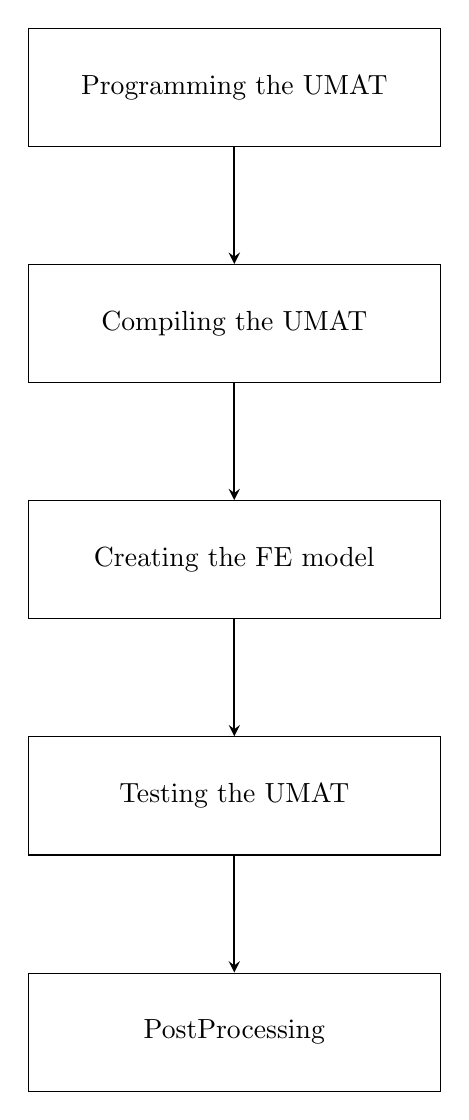
\begin{tikzpicture}[node distance = 3cm]

\node(start) [process] {Programming the UMAT};
\node(compile) [process, below of = start] {Compiling the UMAT};
\node(Model)   [process, below of = compile] {Creating the FE model};
\node(solve) [process, below of = Model] {Testing the UMAT};
\node(post)[process, below of = solve] {PostProcessing};


\draw [arrow] (start) -- (compile);
\draw [arrow] (compile) -- (Model);
\draw [arrow] (Model) -- (solve);
\draw [arrow] (solve) -- (post);


\end{tikzpicture}
\FloatBarrier
\label{Schematic of UMAT implementation}
\end{center}
\vspace*{0.6cm}
\section{Programming the UMAT}
\indent\indent\indent  The user material subroutine is an ANSYS programmable feature which allows users to write their own material constitutive equations within a newly developed general material framework. The subroutine is called at all material integration points of the element during the solution phase.\\
\indent\indent\indent ANSYS demands the necessary variables declared in a certain way so that the USERMAT developed can work compatibly with ANSYS when it is called at each integration point. The guidelines for declaring input and output arguments can be found on ANSYS' usermat guide.  The following image shows the user subroutine interface with the set of possible input arguments that USERMAT can access from ANSYS \\
\begin{figure}[htbp]
\begin{center}
\includegraphics[width=0.7\textwidth]{{9.Usermat_input}}
 \caption{Usermat Interface}
 \label{fig:Usermat Interface}
 \end{center}
\end{figure}
For every Newton raphson iteration, the USERMAT is called at every material integration point, and ANSYS passes in strains, stresses and state variables at the beginning of the time increment and the current strain increment. The USERMAT then has to compute and update the necessary output arguments like stresses and state variables at the end of the increment and the material tangent stiffness matrix $\frac{\partial \sigma}{\partial \epsilon} $.
\vspace*{0.6cm}
\section{Compiling the UMAT}
\indent\indent\indent The user-programmable subroutines must be compiled before testing them in ANSYS environment. The compilation process first checks for errors in the source code and then converts it into ANSYS executable files (.dll files), which can be used by ANSYS. The compiler present in Intel parallel studio is used for this purpose. The step by step process of compiling the UMAT is given below
\begin{itemize}
\item Create an empty directory and copy the usermat file you want to compile (.f files) into the empty directory.
\item Change the name of your usermat file to $usermat$
\item Go to "Control Panel$>$Search System$>$Edit the system environment variables$>$Environment variables" and click New in the user variables for your PC, which opens a window
\item In that window, type ANS\_USER\_PATH for variable name and for variable value, copy and paste the path to your working directory and click Ok
\item Go to folder "C:\texttt{\textbackslash} Program Files\texttt{\textbackslash} ANSYS Inc\texttt{\textbackslash} v181\texttt{\textbackslash} ansys\texttt{\textbackslash} custom\texttt{\textbackslash} user\texttt{\textbackslash} win64" and copy the ANSUSERSHARED.bat file and paste it in the working directory
\item Open command prompt and navigate to the working directory
\item Type ANSUSERSHARED.bat and press enter. This opens the Intel compiler and asks for user-programmable feature source file name
\item Type $usermat$ without extension and press Enter.
\item If there is no error in the usermat file the compiler will show the message "usermatLib.dll has been successfully build."  
\item For ANSYS to access these .dll files, open ANSYS Mechanical APDL product launcher and in the file management section browse to the current working directory
\item Click run and in the Mechanical APDL output window you should see the message "Note - This ANSYS version was linked by Licensee". This indicates that you are using the shared library with the USERMAT\\
\end{itemize} 

\section{Creating FE model}
\indent\indent\indent  The preprocessor section of ANSYS mechanical APDL is used to create and mesh the FE model. The ANSYS user-programmable feature can be used with 18x family elements, which include LINK180, PLANE 182, PLANE 183, SOLID 185, SOLID 186. The type of element required for creating FE models based on the problem can be chosen from the element type menu in the preprocessor section. Once the element type is chosen, the material model, and the material properties can be entered in the $Material\; props$ section.  The $Modelling$ section can be utilised to create the geometry required for testing the subroutines and then can be meshed using the $Meshing$ option.\\ \indent\indent\indent To use the FE model, again and again, to test different material models with different material properties the FE model can be saved in the form of an APDL script.  An APDL script is a simple text file containing the commands required to create and solve the FE model. A simple way to create an APDL script for an FE model is to copy the log of commands automatically created in the log file during the creation of your model and pasting it to a new text file. This log file can be accessed by going to $List>Files>Logfile$. The created APDL script can then be accessed by going to $File>Read \;input\; from$ and navigate and select your file.

\section{Testing the UMAT}
\indent\indent\indent  To use the user material option, the TB,USER command must be included in the APDL script so that the user material can be defined. The table command for USER material option is\\
\\
\textbf{TB,USER,matId,NTEMPS,NPTS}
\\
\\
\indent matId - material reference number
\\
\\
\indent NTEMPS - Number of temperature points 
\\
\\
\indent NPTS  -  Number of material constants at a given temperature
\\
\\
If state variables are used in the subroutine, the number of state variables need to be defined in the APDL script by the command TB,STATE\\
\\
\textbf{TB,STATE,matId,,NPTS}\\
\\
\indent matId - material reference number
\\
\\
\indent NPTS - Number of state variables to be used in USERMAT
\\
\\
A simple example for defining a user material and two state variables is given in the Figure.(\ref{fig:Tb}) below
\begin{figure}[htbp]
\begin{center}
\includegraphics[width=0.3\textwidth]{{12.Tb}}
 \caption{Table (TB) commands}
 \label{fig:Tb}
 \end{center}
\end{figure}
\FloatBarrier
Before defining boundary conditions (BCs), the entities required for solving the FE model, such as time at the end of the load step, the number of steps, the results to be stored etc., must be defined. This can be done using $Sol'n\; Controls$ option in the solution menu. Once the BCs are defined, the model can be solved by giving the command $SOLVE$. 
\vspace*{0.5cm}
\section{PostProcessing}
\indent\indent\indent Once the FE model has finished solving, the results can be analyzed using the 'General Postprocessor' option. The nodal and elemental solution for components like stress, strain, displacement etc., can be plotted using the 'contour plot' option, which can be found on Plot results. By default, this option plots the results at the last substep, so to plot the solution at the substep of one's choice one must navigate to $Read\;results>By\;pick$ and select the substep to be plotted. Since the posprocessor of ANSYS does not have GUI option for plotting state variables the following command must be given: $ plnsol,svar,n $ where $n$ is the number of the state variable to be plotted. The time history of a certain variable, such as stress, reaction force, strain etc., at a node or an element can be plotted using $TimeHist\;Postpro$ option. On clicking the $TimeHist\;Postpro$ option a $Variable\;List$ window opens up. To add the variables to plot, click the green add symbol on the top-left corner which opens a window with the list of variables that can be added to the $Variable\;List$ window. Once the variables have been added, the variables can be plotted against each other or against time. Fig.(\ref{fig:Timehist}) shows the $Variable\;List$ window with X-component of force and displacement of node 3 selected and plotted against each other.
\begin{figure}[htbp]
\begin{center}
\includegraphics[width=0.8\textwidth]{{13.Timehist}}
 \caption{Time history post processor window}
 \label{fig:Timehist}
 \end{center}
\end{figure}
\FloatBarrier
The time history results of each variable at a node or an element can also be saved as a text file using $List\;Data$ option in the 
$Variable\;List$ window. 



\clearpage
\vspace*{7cm}
\chapter{Progressive failure analysis of orthotropic composite materials }
\vspace*{1.5cm}
\section{Fibre-reinforced Composites}
\indent\indent\indent  Fibre-reinforced plastic composites is a term for a large family of materials ranging from short fibre reinforced polyamides to unidirectional graphite fibre epoxies. Fibre-reinforced composites consist of three components 1) the fibres as the discontinuous or dispersed phase, 2) the matrix as the continuous phase, and 3) the fine interphase region, also known as the interface.  The first fibres used in fibre reinforced plastics are made of glass. Although the virgin strength of the glass is high, the actual strength is limited by the microscopic defects on the surface of the fibre. The graphite fibres are anisotropic due to their laminar structure. Graphite fibres maintain their strength even at high temperatures. Two types of plastics are commonly used as matrix materials, namely unsaturated polyesters and epoxies. The use of unsaturated polyesters is restricted to temperatures up to 100C. The main advantage of this material is the high amount of shrinkage at hardening, which causes high internal stress and decrease the strength of the material.  The characteristics of epoxy are better than polyester resins. The material can withstand temperatures up to 250C and shrinks only  2\%  at hardening. However, epoxy resins are high in price compared to polyesters.


\section{Mechanisms of damage and failure in fibre reinforced composites}
\indent\indent\indent The failure in fibre reinforced composites happens mainly due to matrix cracking or fibre failure. Therefore the failure can be divided mainly two types, namely 1) Longitudinal failure and 2) Transverse failure. The mechanism of both failure mechanisms, their causes and their effects on material behaviour are discussed in detail below

\subsection{Longitudinal failure}
\indent\indent\indent  In fibre-reinforced plastics, the most significant portion of the load is carried by fibres. When the fibres fail, the load must redistribute to other areas of the structure and may cause structural collapse. In composites where strain to failure for the resin matrix is higher than the one of the reinforcing fibre, longitudinal failures start by isolated fibre fractures in weak zones. This kind of localized fracture increases the normal and interfacial shear stress in fibres and promotes matrix cracking, fibre matrix debonding, conical shear failures, etc. When the load is further increased, it may lead to the final collapse. Longitudinal tensile failure occurs in both constituents, and a fracture occurs along a plane whose normal is parallel to the fibre direction. Simple maximum stress or maximum strain can usually provide an accurate measure of longitudinal tensile failure. Longitudinal compressive failure occurs from the collapse of the fibres due to shear kinking and damage of the supporting matrix. Fibre misalignment causes shear stress between fibres that rotate fibres, which increases shear stress further and leads to instability. 
 

\subsection{Transverse failure}
\indent\indent\indent   Transverse failure happens due to matrix cracking and fibre-matrix debonding. Under the presence of in-plane shear stress and transverse tensile stress, the combined effects of defects such as resin-rich regions, fibre-resin debonds, and resin voids trigger a transverse crack that extends through the thickness. The transverse cracks are formed at the fibre-resin interface without affecting the fibres. When a unidirectional fibre composite is loaded in shear, a non-linear shear stress-strain behaviour is observed before the material fails by through-thickness matrix cracking. This non-linear behaviour is due to the visco-plastic behaviour of the matrix and from the nucleation of microvoids.\\
\begin{figure}[htbp]
\begin{center}
\includegraphics[width=0.9\textwidth]{{5. FRP failure.png}}
 \caption{Fracture planes in FRP material}
 \label{fig:FRP failure}
 \end{center}
\end{figure}
\indent\indent\indent Experimental results have shown that moderate compression has beneficial effects on the strength of the material (Soden et al., 1998); when the transverse compressive stress value is smaller than the in-plane shear stress, the fracture plane is perpendicular to the mid-plane of the ply. Increasing the compressive stress changes the angle of the fracture plane. For glass-epoxy and carbon-epoxy composites, when loaded in pure transverse compression, the fracture plane is at an angle of 53° $\pm$ 3° with respect to the thickness direction. Therefore, the matrix cracking does not occur in the plane of maximum transverse shear stress (45°).\\

\section{Damage initiation criteria}
\indent\indent\indent   Damage initiation criteria refer to the onset of damage at a material point. Since the properties of  orthotropic materials are different in the mutually perpendicular directions, three failure mode indices, $F_{f}, F_{m}, F_{z}$, are used for failure modes in three principal material directions. Since the failure due to tension and compression in each direction cannot happen at the same integration point and at the same time, the failure mode index must be calculated based on whether the material direction is under tension or compression. Both strain and stress-based damage initiation criteria can be employed based on the application. Some of the damage initiation criteria are given as follows
\subsection{Maximum strain criteria}\label{Maximum strain criteria}
\indent\indent\indent The maximum strain criterion is a simple criterion which checks whether the strain in the given material direction exceeds the failure strain or not. The maximum strain criterion for each material direction is given below\\
\begin{table}[htbp]
  \begin{center}
     \begin{tabular}{l  c  c} 
     \hline
     \\
      \textbf{Damage direction} \;\;& \textbf{Tension} \;& \textbf{Compression}\\
      \\
      \hline
      \\
      Longitudinal direction 1 ($F_{f}$) & \Large{$\frac{\epsilon_{1}}{\epsilon_{t1}} $}\small{ $\leq 1$} &  \Large{$\frac{\epsilon_{1}}{\epsilon_{c1}} $}\small{ $\leq 1$}\\
      \\
      Transverse direction 2 ($F_{m}$)  &  \Large{$\frac{\epsilon_{2}}{\epsilon_{t2}} $}\small{$\leq 1$}  & \Large{$\frac{\epsilon_{2}}{\epsilon_{c2}} $}\small{$\leq 1$}\\
      \\
      Thickness direction 3 ($F_{z}$) &  \Large{$\frac{\epsilon_{3}}{\epsilon_{t3}} $}\small{$\leq 1$}  &   \Large{$\frac{\epsilon_{2}}{\epsilon_{c3}} $}\small{$\leq 1$}\\
       \\
       \hline
    \end{tabular}
    \\
    \caption{Maximum strain criterion}
    \label{tab:Maximum strain criterion}
  \end{center}
\end{table}
\FloatBarrier
where $\epsilon_{ti}$ and $\epsilon_{ci}$ are failure strains in tension and compression respectively, in each material direction. 
\\
\subsection{Maximum stress criteria}\label{Maximum stress criteria}
\indent\indent\indent  Since the load-carrying area decreases due to an increase in damage, the effect of stress gets magnified in the damaged material. Therefore, in the case of maximum stress criteria, normal stress components of the effective stress($\tilde{\sigma}$) are checked against the failure strength in each principal material direction. The effective stress can be computed using the eqn.(\ref{eqn:effective_stress_tensor}). The maximum stress criteria for each material direction are given in the table below\\
\begin{table}[htbp]
  \begin{center}
     \begin{tabular}{l  c  c} 
     \hline
     \\
      \textbf{Damage direction} \;\;& \textbf{Tension} \;& \textbf{Compression}\\
      \\
      \hline
      \\
      Longitudinal direction 1 ($F_{f}$) & \Large{$\frac{\tilde{\sigma}_{11}}{X_{T}} $}\small{ $\leq 1$} & \Large{$\frac{\tilde{\sigma}_{11}}{-X_{C}} $}\small{ $\leq 1$} \\
      \\
      Transverse direction 2 ($F_{m}$)  &  \Large{$\frac{\tilde{\sigma}_{22}}{Y_{T}} $}\small{ $\leq 1$}  & \Large{$\frac{\tilde{\sigma}_{22}}{-Y_{C}} $}\small{ $\leq 1$}\\
      \\
      Transverse direction 3 ($F_{z}$) &  \Large{$\frac{\tilde{\sigma}_{33}}{Z_{T}} $}\small{ $\leq 1$}  &   \Large{$\frac{\tilde{\sigma}_{33}}{-Z_{C}} $}\small{ $\leq 1$}\\
       \\
       \hline
    \end{tabular}
    \\
    \caption{Maximum stress criterion}
    \label{tab:Maximum stress criterion}
  \end{center}
\end{table}
\FloatBarrier
where $X_{T}$,$ Y_{T} $ and $Z_{T}$ are failure strength in tension and $X_{C}$,$ Y_{C} $ and $Z_{C}$ are failure strength in compression in each principal material direction respectively.\\
\\

\subsection{3D Hashin's quadratic strain criteria}\label{3D Hashin's quadratic strain criteria}
\indent\indent\indent Hashin's quadratic strain criteria includes shear strain components in addition to the normal strain components. The criteria for each material direction is given below\\

i) Longitudinal direction 1 ,
\\
\begin{equation}
\large{F_{f}^{2} =  
	\begin{cases}
	
		\Big(\frac{\epsilon_{11}}{\epsilon_{11}^{f,t}}\Big)^{2} \; + \; \Big(\frac{\epsilon_{12}}{\epsilon_{12}^{f}}\Big)^{2} \; + \; \Big(\frac{\epsilon_{13}}{\epsilon_{13}^{f}}\Big)^{2} \; \geq  \; 1  \; \; \; \; \;  (\epsilon_{11}  >  0)  \\
	\\
	\Big(\frac{\epsilon_{11}}{\epsilon_{11}^{f,c}}\Big)^{2}  \; \geq  \; 1 \; \; \; \; \; \; \;  \; \; \; \;  (\epsilon_{11}  <  0) 

	
	\end{cases}}
\end{equation}
\\
\\
ii) Transverse direction 2,
\\
\begin{equation}
\large{F_{m}^{2} =  
	\begin{cases}
	
	\frac{(\epsilon_{22} + \epsilon_{33} )^{2}}{\epsilon_{22}^{f,t} \epsilon_{33}^{f,t}}   -  \frac{\epsilon_{22}\epsilon_{33}}{(\epsilon_{23}^{f})^{2}}  +  \Big(\frac{\epsilon_{12}}{\epsilon_{12}^{f}}\Big)^{2}  + \Big(\frac{\epsilon_{13}}{\epsilon_{13}^{f}}\Big)^{2}  +  \Big(\frac{\epsilon_{23}}{\epsilon_{23}^{f}}\Big)^{2} \;\geq  \; 1 \; \; \; \; \;  (\epsilon_{22}  >  0) \\
	\\
	
	\frac{(\epsilon_{22} + \epsilon_{33} )^{2}}{\epsilon_{22}^{f,c} \epsilon_{33}^{f,c}}  +  \frac{\epsilon_{22} + \epsilon_{33}}{\epsilon_{22}^{f,c}}\Big(\frac{\epsilon_{22}^{f,c}}{2\epsilon_{12}^{f}}  -  1\Big)   -  \frac{\epsilon_{22}\epsilon_{33}}{(\epsilon_{23}^{f})^{2}}  +  \Big(\frac{\epsilon_{12}}{\epsilon_{12}^{f}}\Big)^{2}\; \; \; \; \; \; \; \; \; \; \; \;  (\epsilon_{22}  >  0) \\ 
\\	
	\; \; \; \; \; \; \; \;\; \; \; \; \; \; \; \;\; \; \; \; \; \; \; \;  \; \;\; \; \; \; \; \; \; \;\; \; \; \; \;  + \Big(\frac{\epsilon_{13}}{\epsilon_{13}^{f}}\Big)^{2}   +  \Big(\frac{\epsilon_{23}}{\epsilon_{23}^{f}}\Big)^{2} \;\geq \; 1 
	
	
	\end{cases}}
\end{equation}
\\
\\
iii) Transverse direction 3,
\\
\begin{equation}
\large{F_{z}^{2} =  
	\begin{cases}

	\Big(\frac{\epsilon_{33}}{\epsilon_{33}^{f,t}}\Big)^{2} \; + \; \Big(\frac{\epsilon_{13}}{\epsilon_{13}^{f}}\Big)^{2} \; + \; \Big(\frac{\epsilon_{23}}{\epsilon_{23}^{f}}\Big)^{2} \; \geq  \; 1 \; \; \; \; \;  (\epsilon_{33}  >  0) \\

\\
	\Big(\frac{\epsilon_{33}}{\epsilon_{33}^{f,c}}\Big)^{2} \; + \; \Big(\frac{\epsilon_{13}}{\epsilon_{13}^{f}}\Big)^{2} \; + \; \Big(\frac{\epsilon_{23}}{\epsilon_{23}^{f}}\Big)^{2} \; \geq  \; 1 \; \; \; \; \;  (\epsilon_{33}  >  0) \\



	\end{cases}}
\end{equation}
\\
\\
in which  $\LARGE{\epsilon_{ii}^{f,t}=\frac{\sigma_{i}^{f,t}}{C_{ii}}}$,  $\epsilon_{ii}^{f,c}  =   \frac{\sigma_{i}^{f,c}}{C_{ii}} \; (i = 1,2,3)$,  $\epsilon_{12}^{f}  =   \frac{\sigma_{12}^{f}}{C_{44}}$,   $\epsilon_{13}^{f}  =  \frac{\sigma_{13}^{f}}{C_{55}}$,  $\epsilon_{23}^{f}  =   \frac{\sigma_{23}^{f}}{C_{66}}$

\subsection{Modified Hashin's failure criterion}\label{Modified Hashin's failure criterion}
\indent\indent\indent Modified Hashin's failure criterion for plane stress condition is given below
\\
\\
i) Longitudinal direction 1,
\\
\begin{equation}
\large{F_{f} =  
	\begin{cases}
	
		\left[ \Big(\frac{\tilde{\sigma_{11}}} {X_{T}}\Big)^{2} \; + \;\alpha . \Big(\frac{\tilde{\sigma_{12}}}{S}\Big)^{2}\right]^{\frac{1}{2}} \;  \geq  \; 1  \; \; \; \; \;  (\tilde{\sigma_{11}}  >  0)  \\
	\\
\left[ \Big(\frac{\tilde{\sigma_{11}}} {X_{C}}\Big)^{2} \; + \;\alpha . \Big(\frac{\tilde{\sigma_{12}}}{S}\Big)^{2}\right]^{\frac{1}{2}} \;  \geq  \; 1  \; \; \; \; \;  (\tilde{\sigma_{11}}  <  0)
	
	\end{cases}}
\end{equation}
\\
\\
i) Transverse direction 2,
\\
\begin{equation}
\large{F_{f} =  
	\begin{cases}
	
	\left[ 	\Big(\frac{\tilde{\sigma_{22}}} {Y_{T}}\Big)^{2} \; + \;\alpha . \Big(\frac{\tilde{\sigma_{12}}}{S}\Big)^{2} \right]^{\frac{1}{2}} \;  \geq  \; 1  \; \; \; \; \;  (\tilde{\sigma_{22}}  >  0)  \\
	\\
\left[ \Big(\frac{\tilde{\sigma_{22}}} {Y_{C}}\Big)^{2} \; + \;\alpha . \Big(\frac{\tilde{\sigma_{12}}}{S}\Big)^{2}\right]^{\frac{1}{2}} \;  \geq  \; 1  \; \; \; \; \;  (\tilde{\sigma_{22}}  <  0)
	
	\end{cases}}
\end{equation}
\\
\\
where the shear contribution factor $\alpha$ ranges from 0 to 1.

\section{Types of damage evolution}
\indent\indent\indent Once the damage is initiated in a material point of composite material, the stiffnessmust be degraded. This results in strain-softening of the composite materials rather than strain hardening, which is observed in metals. Several post-damage models have been proposed for progressive failure analysis, and most of them belong to one of the following categories: instantaneous unloading, gradual loading, or constant stress at failure material point, as shown in Fig.(\ref{fig:Types_of_damage_evolution}) \\  
\indent\indent\indent Since continuum damage mechanics is a methodology to predict the progressive failure behaviour of composites, non-linear gradual unloading of the composite material is adopted and simulated in this work.  Therefore non-linear material properties degradation model is implemented in this work. Based on the type of damage variable chosen, i.e., scalar, vector or second-order tensor, the damage modelling can be classified into isotropic or anisotropic damage modelling. A brief description of the types of damage modelling, damage evolution equation used and material tangent stiffness etc. is given below

\begin{figure}[htbp]
\begin{center}
\includegraphics[width=0.7\textwidth]{{8.Types_of_damage_evolution}}
 \caption{Types of degradation behaviour in damaged composite materials}
 \label{fig:Types_of_damage_evolution}
 \end{center}
\end{figure}


\subsection{Isotropic damage}
\indent\indent\indent In the case of isotropic distribution of cracks, the damage state is usually considered isotropic, and only a scalar variable $D$ is required to represent the damage state of the material. In this work, a damage evolution law of the following form is considered for calculating damage, once the damage has been initiated
\\
\\
\begin{equation}
  \large{ D \; = \; 1 - e^{-P(\tilde{\epsilon} - k)}}
  \label{eqn: isotropic_damage}
\end{equation} 
\\
where $P$ is the softening parameter which determines the slope of the damage evolution, $\tilde{\epsilon}$ is the 1D equivalent strain and $k$ is the threshold value. Since the eqn. (\ref{eqn: isotropic_damage}) is an exponential equation, the damage D evolves exponentially from 0 to 1, and the strain-softening will be an exponential decay function. Once the damage starts to evolve, the material property must be degraded. Therefore the material stiffness matrix of the  damaged material is given by,\\
\begin{equation}
\large{\mathbb{C}(D) \; = \; (1  - D) \mathbb{C}_{0} }
\end{equation} 
where $\mathbb{C}_{0}$ is the material stiffness matrix of the undamaged material. Therefore the stress-strain relation for a strain softening model is given by,\\
\begin{equation}
\large{\sigma \; = \; \mathbb{C}(D) : \epsilon }  
\end{equation}
\\
The finite element equations obtained for the strain-softening model are non-linear. Therefore Newton-Raphson technique is used to solve the resulting system of non-linear equations. To ensure the robustness of the Newton-Raphson method, it is important to compute the material tangent constitutive tensor $\mathbb{C}_{T}$. It can be derived as follows,\\
\begin{equation*}
\large{ \mathbb{C}_{T}  \; = \;\frac{\partial \sigma}{\partial \epsilon}  }
\end{equation*}

\begin{equation*}
\large{\sigma  \; = \; f(\epsilon, D) }
\end{equation*}

\begin{equation}
\large{\mathbb{C}_{T}  \; = \; \mathbb{C}(D) + \epsilon : \Big(\frac{\partial \sigma }{\partial D} \otimes \frac{\partial D}{\partial \epsilon}  \Big)    }
\end{equation}
\\
In the above equation, the first term $\mathbb{C}(D)$ is the damaged elasticity matrix and second term is due increased damage. In the absence of damage propagation in an increment(For eg., during unloading), the material tangent tensor is equal to the damaged elasticity matrix, so the response is linearly elastic.
\subsection{Anisotropic damage}
\indent\indent\indent In the case of orthotropic materials, the material property differs in the mutually perpendicular directions. Therefore it is more appropriate to choose a second-order damage tensor. In this work, a symmetric second-order tensor $\underline{D}$ is chosen, whose principal directions are assumed to coincide with the principal material directions. The eigenvalues of the damage tensor $\underline{D}$ have a simple physical interpretation, i.e., the $i^{th}$ eigenvalue $d_{i}$ represents the effective fractional reduction in load carrying area on planes that are perpendicular to $i^{th}$ principal material direction. The damage tensor $\underline{D}$ can be represented as,
\\
$$
\underline{D} \; = \; 
 \begin{bmatrix}
  d_{1}  \;& 0  \; & 0  \\
  \\
  0 \; & d_{2} \; & 0  \\
  \\  
  0 \; & 0 \; & d_{3} \\
  
 \end{bmatrix}
 $$  
\\
The relationship between damaged and undamaged material must be established so that it helps us derive the constitutive equation (i.e., damaged elastic stiffness matrix) for the damaged material. In this work, the hypothesis of strain energy equivalence (Section.\ref{Hypothesis of strain energy equivalence}) is used to derive the elastic stiffness matrix of the damaged material. According to the hypothesis of strain energy equivalence, from Eqn. (\ref{eqn: S_HSEeq}) the elastic stiffness matrix of the damaged material can be derived as,\\
\begin{equation}
\mathbb{C}(D) \; = \; \mathbb{M}^{-1} : \mathbb{C}_{0} :  \mathbb{M}^{T,-1}  
\label{Damaged_elasticity_matrix_1}
\end{equation}
where $\mathbb{M}$ is the damage effect tensor from Section.(\ref{Matrix Representation of Damage effect tensors}). Refer to sections  and  for the matrix representation of the damaged elastic stiffness matrix for both transversely isotropic (2D/Plane-stress) and orhtotropic materials (3D) 

A simple damage evolution law for each principal material direction in case of anisotropic damage is given as follows,
\begin{equation}
d_{i} = 1 - \frac{e^{-P(F_{I} - 1)} }{F_{I}}  
\label{exponential damage equation}
\end{equation}
where $d_{i}$ (i = 1,2,3) and $F_{I}$ (I = f,m,z) are damage evolution and failure index in each principal material direction respectively.
The material tangent stiffness tensor for anisotropic damage can also be derived in the same way as isotropic damage and it is given as follows
\begin{equation*}
\large{ \mathbb{C}_{T}  \; = \;\frac{\partial \sigma}{\partial \epsilon}  }
\end{equation*}

\begin{equation*}
\large{\sigma  \; = \; f(\epsilon, \underline{D}) }
\end{equation*}

\begin{equation}
\mathbb{C}_{T}  \; = \; \mathbb{C}(D) + \epsilon : \sum_{i = 1}^{3}  \Big( \frac{\partial \sigma }{\partial d_{i}} \otimes \frac{\partial d_{i}}{\partial \epsilon }\Big)
\label{Anisotropic tangent stiffness} 
\end{equation}
In the above equation, the second term(i.e., due to increased damage) must be computed only if the corresponding failure mode is active. Since the damage evolution equation $d_{i}$ depends on the failure index, the term $\frac{\partial d_{i}}{\partial \epsilon }$ must be computed based on whether the corresponding damage happened during tension or compression.

\section{Localisation and Mesh Regularisation}\label{Mesh Regularisation}
\indent\indent\indent Finite element simulations which use continuum damage models are susceptible to mesh dependency. When the finite element discretization is refined, the numerical problems do not converge to a physically meaningful solution. Because of the strain-softening behaviour of the material, the strain tends to localize, resulting in a strong mesh dependency, i.e., the solution is non-objective with respect to mesh refinement, and the energy dissipated decreases with the decrease in finite element size. Merely improving the numerical solution schemes cannot alleviate the problem associated with mesh dependency and localization. Even if the convergence to the actual solution is improved, the solution may not even make sense from a physical point of view. Therefore the so-called fracture energy regularization is used to reduce the mesh sensitivity. In this technique, the softening law (damage evolution law) is modified so that the amount of energy dissipated over a fully degraded finite element depends on the fracture energy of the material and the finite element size. Therefore the fracture energy ($G_f$) of the material and characteristic length ($L_{c}$) of the finite element must be included in the damage evolution equations. The damage evolution equations based on fracture energy regularization technique for each principal direction is shown below, \\
\\
In longitudinal direction 1,
\begin{equation}
\label{d1}
\mathlarger{d_{1} = 1 - \frac{e^{P_{1}(F_{f} - 1)}}{F_{f}}}
\end{equation}
\\
In transverse direction 2,
\begin{equation}
\label{d2}  
\mathlarger{d_{2} = 1 - \frac{e^{P_{2}(F_{m} - 1)}}{F_{m}}}
\end{equation}
\\
In transverse direction 3,
\begin{equation}
\label{d3} 
\mathlarger{d_{3} = 1 - \frac{e^{P_{3}(F_{z} - 1)}}{F_{z}}}
\end{equation}
\\
\\
\\
where $\mathlarger{P_{1} = \frac{-\sigma_{11}^{f}\epsilon_{11}^{f}L_{c}}{G_{f,1}}}$, $\mathlarger{P_{2} = \frac{-\sigma_{22}^{f}\epsilon_{22}^{f}L_{c}}{G_{f,2}}}$ and $\mathlarger{P_{3} = \frac{-\sigma_{33}^{f}\epsilon_{33}^{f}L_{c}}{G_{f,3}}}$ 
\\ 
\\ 
\\
$\mathlarger{G_{f,i}}$ \; - \;is the fracture energy in each principal direction (i = 1,2,3)  \\ $\mathlarger{\sigma_{ii}^{f}}$ \;\;\; -  \;  failure strength in each principal direction (i = 1,2,3) \\ $\mathlarger{\epsilon_{ii}^{f}}$\;\;\;\;\; - \; failure strain in each principal direction (i = 1,2,3) \\ $\mathlarger{L_{c}}$\;\;\;\;\; - \; Characteristic length

\section{Numerical implementation of the damage model in ANSYS}
\indent\indent\indent  As discussed before, the material models necessary for simulating progressive damage failure are implemented using the ANSYS user-programmable feature called USERMAT. The damage model implemented using USERMAT computes and updates the current stress and consistent tangent stiffness. The following sections deal with the numerical implementation of the damage model based on two different methods or criteria used to predict the damage initiation.
\\
\begin{itemize}
\item Strain based damage model 
\item Stress based damage model 
\end{itemize}
\subsection{Strain based damage model}
\indent\indent\indent  In the case of the strain-based damage model, the damage initiation is predicted using current strain ($\epsilon_{n+1}$).   The USERMAT receives strains, stresses and state variables at the beginning of the time increment and the current strain increment. The following steps describe the process of implementing the damage model


\begin{itemize}
\item Calculate current strain \textbf{$$ \underline{\epsilon}_{n+1} = \underline{\epsilon}_{n} + \underline{\Delta \epsilon} $$}
\item Calculate the current degraded material stiffness matrix  \textbf{$\mathbb{C}(\underline{D}_{n})$}
\item Calculate the failure indices \textbf{$F_{I}(\underline{\epsilon})$} \;\; ( Refer to Sections (\ref{Maximum strain criteria}) and (\ref{3D Hashin's quadratic strain criteria}) )
\item[] Check if $F_{I} \geq F_{I}$max
\item if \textbf{$F_{I}(\underline{\epsilon})<1$} \textbf{$$\underline{\sigma}_{n+1} \; = \; \mathbb{C}(\underline{D}_{n}) :  \underline{\epsilon}_{n+1} $$} \textbf{$$\mathbb{C}_{T} \; = \; \mathbb{C}(\underline{D}_{n})$$}
\item else
\item[]  Calculate the damage variables using damage evolution law, \;\; ( Refer to eqn (\ref{d1}) to (\ref{d3}) ) \textbf{$$d_{1}(F_{f}),\;d_{2}(F_{m}),\;d_{3}(F_{z})$$}
\item[]  Check if $d_{i} \geq 0 $ 
\item[]  Calculate the updated degraded stiffness based on damage variables \textbf{$$\mathbb{C}(\underline{D}_{n+1})$$}
\item[]  Calculate current stress  \textbf{$$\underline{\sigma}_{n+1} \; = \; \mathbb{C}(\underline{D}_{n+1}) :  \underline{\epsilon}_{n+1} $$}
\item[] Calculate tangent stiffness \textbf{$$\mathbb{C}_{T}  \; = \;\mathbb{C}(D) + \sum_{i = 1}^{3} \Big( \frac{\partial \mathbb{C}(D) }{\partial d_{i}} : \epsilon \otimes \frac{\partial d_{i}}{\partial \epsilon }\Big)$$}
	
\end{itemize} 


\subsection{Stress based damage model}
\indent\indent\indent  In the case of stress-based damage model, the damage initiation is predicted using effective stress ($\underline{\tilde{\sigma}}_{n+1}$).  The USERMAT receives strains, stresses and state variables at the beginning of the time increment and the current strain increment. The following steps describe the process of implementing the damage model.

\begin{itemize}
\item Calculate the elastic stiffness matrix  \textbf{$\mathbb{C}$}
\item Calculate effective stress \textbf{$$\underline{\tilde{\sigma}}_{n+1} = \mathbb{C}_{0} : \underline{\epsilon}_{n+1} $$}
\item Calculate the failure indices \textbf{$F_{I}(\underline{\sigma})$},\;\; ( Refer to Section (\ref{Maximum stress criteria}) and (\ref{Modified Hashin's failure criterion}) )
\item[] Check if $F_{I} \geq F_{I}$max
\item if \textbf{$F_{I}(\underline{\sigma})<1$} \textbf{$$\underline{\sigma}_{n+1} \; = \; \underline{\tilde{\sigma}}_{n+1} $$} \textbf{$$\mathbb{C}_{T} \; = \; \mathbb{C}$$}
\item else
   	
\item[]  Calculate the damage variables using damage evolution law, \;\; ( Refer eqn (\ref{d1}) to (\ref{d3}) )  \textbf{$$d_{1}(F_{f}),\;d_{2}(F_{m}),\;d_{3}(F_{z})$$}  	
\item[]  Check if $d_{i} \geq 0 $ 
\item[]  Calculate the updated degraded stiffness based on damage variables \textbf{$$\mathbb{C}(\underline{D}_{n+1})$$}
\item[]  Calculate current stress  \textbf{$$\underline{\sigma}_{n+1} \; = \;  M(D)^{-1}:\underline{\tilde{\sigma}}_{n+1} $$}
\item[] Calculate tangent stiffness \textbf{$$\mathbb{C}_{T}  \; = \;\mathbb{C}(D) + \sum_{i = 1}^{3} \Big( \frac{\partial \mathbb{C}(D) }{\partial d_{i}} : \epsilon \otimes \frac{\partial d_{i}}{\partial \epsilon }\Big)$$}
	
\end{itemize} 

\newpage
\section{Schematic of UMAT implementation}
\indent\indent\indent The flowchart below shows the schematic of the user material subroutine (USERMAT) implementation for both and strain and stress based damage model and how the subroutine interacts with the ANSYS environment.

\begin{center}
\begin{adjustbox}{max height=1.35\textwidth,center}
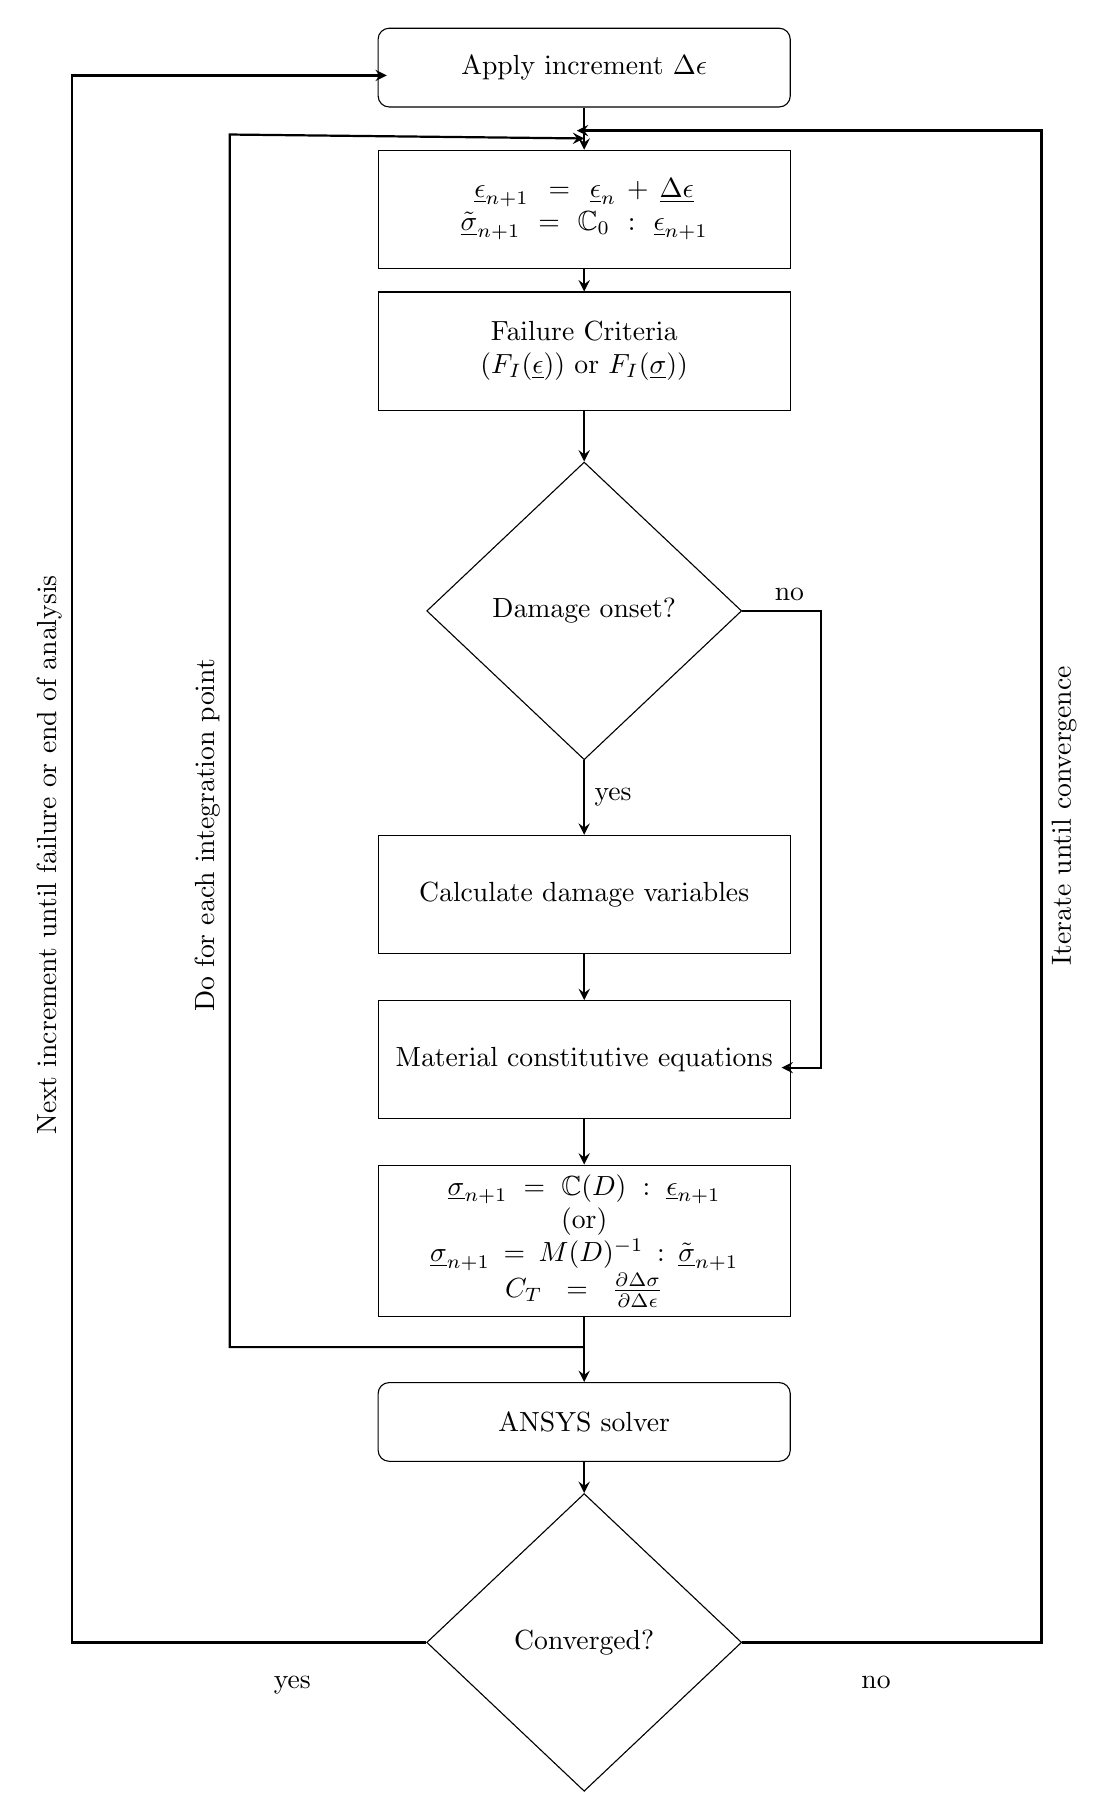
\begin{tikzpicture}[node distance = 1.8cm]

\node(straininc) [startstop] {Apply increment $\Delta\epsilon$};
\node(strainadd) [process, below of = straininc] {$\underline{\epsilon}_{n+1} = \underline{\epsilon}_{n} + \underline{\Delta\epsilon} $ \\ $\underline{\tilde{\sigma}}_{n+1} = \mathbb{C}_{0} : \underline{\epsilon}_{n+1} $};
\node(Failure)   [process, below of = strainadd] {Failure Criteria ($F_{I}(\underline{\epsilon}))$ or $F_{I}(\underline{\sigma}))$ };
\node(Damageon)  [decision, below of = Failure, yshift=-1.5cm] {Damage onset?};
\node(Damagecalc) [process, below of = Damageon, yshift=-1.8cm] {Calculate damage variables};
\node(Materialeqn)[process, below of = Damagecalc, yshift=-0.3cm] {Material constitutive equations};
\node(Tangent)[process, below of = Materialeqn, yshift=-0.5cm] { $\underline{\sigma}_{n+1} = \mathbb{C}(D):\underline{\epsilon}_{n + 1}$ \\ (or) \\$\underline{\sigma}_{n+1} = M(D)^{-1}:\underline{\tilde{\sigma}}_{n+1}$ \\ $C_{T}=\frac{\partial \Delta \sigma}{\partial \Delta \epsilon}$};
\node(abaqus)[startstop, below of = Tangent, yshift=-0.5cm] {ANSYS solver};
\node(Converge)[decision, below of = abaqus, yshift=-1cm] {Converged?};

\draw [arrow] (straininc) -- (strainadd);
\draw [arrow] (strainadd) -- (Failure);
\draw [arrow] (Failure) -- (Damageon);
\draw [arrow] (Damageon) -- node[anchor = west]{yes} (Damagecalc);
\draw [arrow] (Damagecalc) -- (Materialeqn);
\draw [arrow] (Materialeqn) -- (Tangent);
\draw [arrow] (Tangent) -- (abaqus);
\draw [arrow] (abaqus) -- (Converge);
\draw [arrow] (Damageon.east) node[xshift=0.6cm,anchor = south]{no} -| ++(1,-5.8) -- ++(-0.5,0)  (Materialeqn);

\draw [arrow] (Converge.west)node[xshift=-1.7cm,yshift=-0.3cm,anchor = north]{yes} -| node[xshift=10cm,sloped,above]{Next increment until failure or end of analysis}++(-4.5,19.9) -- ++ (4,0) (straininc); 

\draw [arrow] (Converge.east)node[xshift=1.7cm,yshift=-0.3cm,anchor = north]{no} -| node[xshift=10.5cm,sloped,below]{Iterate until convergence} ++(3.8,19.2)-- ++ (-5.9,0)  (straininc); 

\draw [arrow] (0,-16.25)-|node[xshift=6.5cm,sloped,above]{Do for each integration point}++(-4.5,15.4)--(-0,-0.9);
 
\end{tikzpicture}
\end{adjustbox}
\end{center}


\newpage

\chapter{Results and Discussion}
\section{Modelling linear elastic behaviour of orthotropic materials}
\indent\indent\indent Before implementing the damage behaviour in orthotropic materials, their linear elastic behaviour must implemented which describes what happens before the damage initiation. As mentioned before orthtoropic materials are a special class of material whose properties differ in mutually perpendicular directions. Therefore 9 independent material constants are required to model their elastic behaviour. Table (\ref{tab:Material parameters(Integration point studies}) summarises the utilised material parameters. The material parameters presented here belongs to an unidirectional glass fiber-reinforced epoxy material. In this material, the strength in the longitudinal direction ($X_{t}$ and $X_{c}$) is very high compared to the transverse directions ($Y_{t}$ and $Y_{c}$) because the fibers are aligned parallel to the longitudinal direction. The constitutive matrix given in the section (\ref{Constitutive matrix}) and Hooke's law help us model the elastic behaviour of the orthotropic materials.\\ 
\begin{figure}[htbp!]
\begin{center}
\includegraphics[width=9cm,height=9cm,keepaspectratio]{{14.Linear_SvsE.png}}
 \caption{Stress-Strain relation (Standard vs user-defined material routine)}
 \label{fig:Stress-Strain Linear elastic}
 \end{center}
\end{figure}
\FloatBarrier
\indent\indent\indent The linear elastic behaviour of the orthotropic material is implemented in the USERMAT using constitutive equations, and in this section, the results obtained are compared against the standard orthotropic material option present in ANSYS using a structural example. A bar of length 10 mm and area 1 mm$^2$ (b = 1 mm, t =1 mm) fixed at one end is chosen for the analysis. The bar is constructed using 8 node SOLID 185 elements, and full integration has been used. A displacement of 1 mm is applied at the free end, and the results obtained using the standard and the user-defined material routines are presented below. Figure (\ref{fig:Stress-Strain Linear elastic}) compares the stress-strain relation of the bar obtained using both ANSYS default and USERMAT 

\begin{table}
  \begin{center}
   \resizebox{\columnwidth}{4.85cm}{
     \begin{tabular}{l l l} 
     \hline
     \\
      \textbf{Symbol} \;\;& \textbf{Material Parameter} \;& \textbf{Value}\\
      \\
      \hline
      \\
      \vspace*{0.1cm}
      $E_{1}$ & Elastic modulus in longitudinal (1) direction &  55000e6 $N/m^{2}$\\
      \vspace*{0.1cm}
      $E_{2}$ = $E_{3}$  & Elastic modulus in transverse (2 and 3) directions   & 9500e6 $N/m^{2}$ \\
      \vspace*{0.1cm}
      $\nu_{12}$ = $\nu_{13}$  & Poisson's ratio (in-plane)  & 0.33 \\
      \vspace*{0.1cm}
      $\nu_{23}$   & Poisson's ratio (Planes 2-3)  & 0.27 \\
      \vspace*{0.1cm}
      $G_{12}$ = $G_{13}$  & In-plane shear modulus  & 5500e6 $N/m^{2}$ \\
      \vspace*{0.1cm}
      $G_{23}$   & Shear modulus (Planes 2-3)   & 3000e6 $N/m^{2}$ \\
      \vspace*{0.1cm}
      $X_{t}$ &  Tensile strength in longitudinal (1) direction  &  2500e6 $N/m^{2}$\\
      \vspace*{0.1cm}
      $X_{c}$ & Compressive strength in longitudinal (1) direction &  -2000e6 $N/m^{2}$\\
      \vspace*{0.1cm}
      $Y_{t}$ & Tensile strength in transverse (2 and 3) directions &  50e6 $N/m^{2}$\\
      \vspace*{0.1cm}
      $Y_{c}$ & Compressive strength in transverse (2 and 3) directions &  -200e6 $N/m^{2}$\\
      \vspace*{0.1cm}
      $S_{12}$ & In-plane strength &  50e6 $N/m^{2}$\\
       \hline
    \end{tabular}
    }
    \\
    \caption{Material parameters (Integration point studies)}
    \label{tab:Material parameters(Integration point studies}
  \end{center}
\end{table}
\FloatBarrier

\begin{figure}[htbp!]
     \captionsetup[subfigure]{justification=centering}
     \begin{subfigure}[b]{0.4\textwidth}
         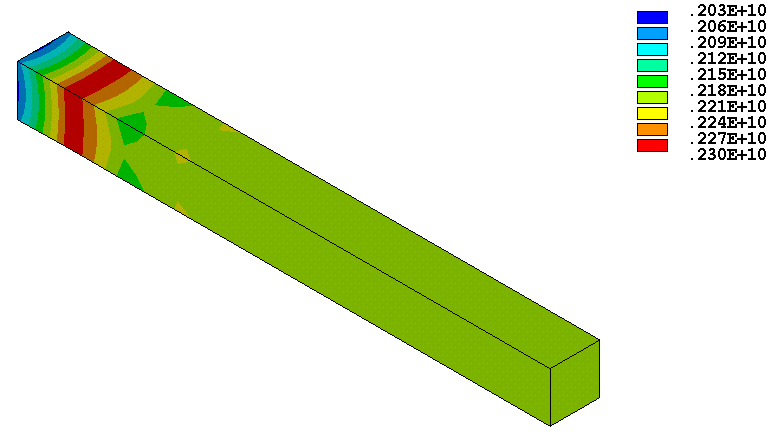
\includegraphics[width=8.3cm,height=8cm,keepaspectratio]{15.Ansys_SX.png}
         \caption{X Component of Stress}
         \label{fig:X Component of Stress}
     \end{subfigure}
     \hspace{1.8cm}
     \begin{subfigure}[b]{0.4\textwidth}
         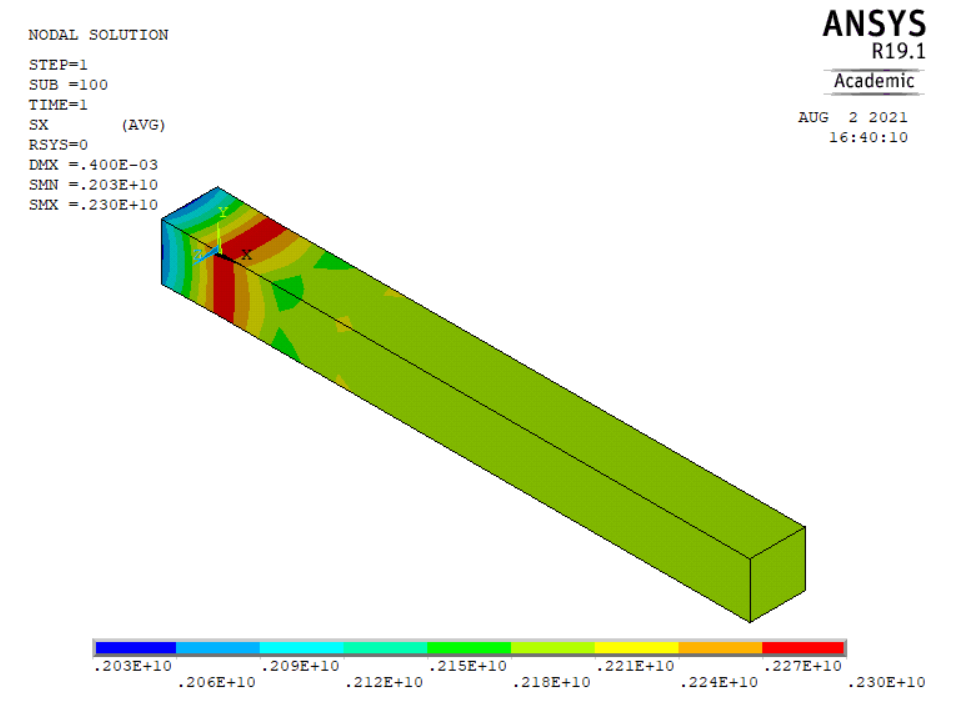
\includegraphics[width=8.3cm,height=8cm,keepaspectratio]{18.User_SX.png}
         \caption{X Component of Stress}
         \label{fig:X Component of Stress2}
     \end{subfigure}
\end{figure}
\FloatBarrier
\begin{figure}[htbp!]\ContinuedFloat     
     \begin{subfigure}[b]{0.4\textwidth}
        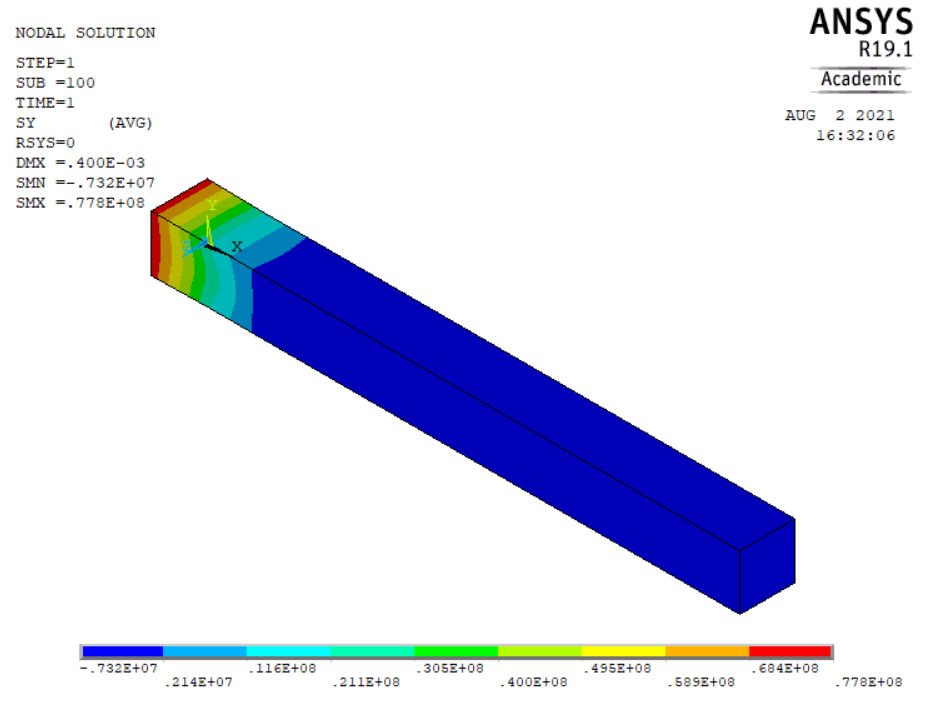
\includegraphics[width=8.3cm,height=8cm,keepaspectratio]{16.Ansys_SY.png}
         \caption{Y Component of Stress}
         \label{fig:Y Component of Stress}
     \end{subfigure}
    \hspace{1.8cm}
      \begin{subfigure}[b]{0.4\textwidth}
         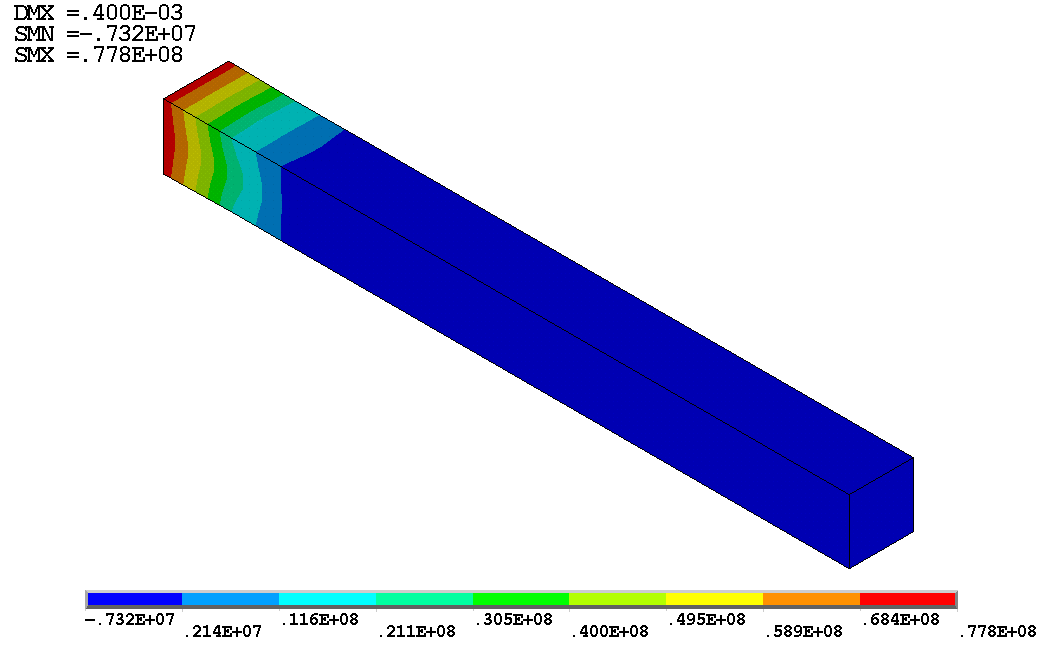
\includegraphics[width=8.3cm,height=8cm,keepaspectratio]{19.User_SY.png}
         \caption{Y Component of Stress}
         \label{fig:Y Component of Stress2}
     \end{subfigure}
\end{figure}
\FloatBarrier
\begin{figure}[htbp!]\ContinuedFloat     
     \begin{subfigure}[b]{0.4\textwidth}
         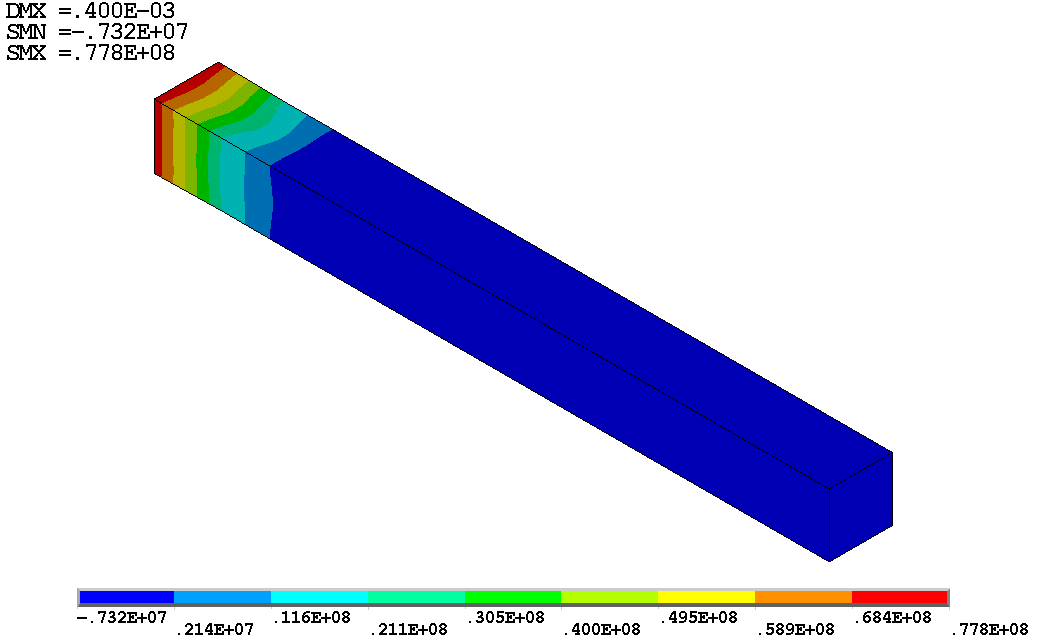
\includegraphics[width=8.3cm,height=8cm,keepaspectratio]{17.Ansys_SZ.png}
         \caption{Z Component of Stress}
         \label{fig:Z Component of Stress}
     \end{subfigure}
     \hspace{1.8cm}
     \begin{subfigure}[b]{0.4\textwidth}
         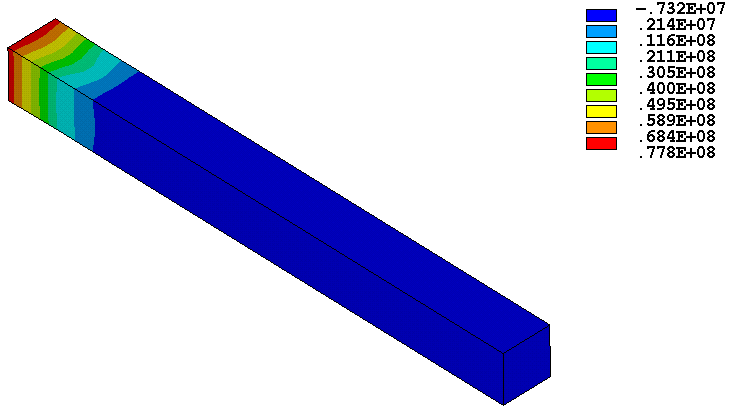
\includegraphics[width=8.3cm,height=8cm,keepaspectratio]{20.User_SZ.png}
         \caption{Z Component of Stress}
         \label{fig:Z Component of Stress2}
     \end{subfigure}
        \caption{Contour plots of the stress components $\sigma_{11}$,$\sigma_{22}$ and $\sigma_{33}$ of the bar obtained using standard (Figures a,c,e on the left) and user-defined material routine (Figures b, d, f on the right)}
        \label{fig:USERMAT}     
\end{figure}
\FloatBarrier

Figure (\ref{fig:USERMAT}) shows the contour plots of the normal stresses ($\sigma_{11}$, $\sigma_{22}$ and $\sigma_{33}$ ) computed using standard and user-defined material routine respectively. The comparison of the stress-strain relation and contour plots between the standard and user-defined material routine confirms that the results obtained using both options are same and therefore further damage-intiation and damage-evolution processes can now be implemented.
\section{Damage behaviour at integration point level}
\indent\indent\indent The material subroutines are first developed on the OCTAVE and tested using constitutive driver routines, enabling us to understand the phenomenon at the integration point level. To demonstrate the evolution of damage after damage initiation and the strain-softening, following simple loading cases are investigated at the integration point level.
\begin{itemize}
\item Uniaxial tension
\item Biaxial tension
\item Triaxial tension.
\end{itemize} 
After that, the material subroutines are implemented in USERMAT and tested in the ANSYS environment using a 3D finite element of unit length. The finite element is subjected to the above loading cases, and the results are compared against the OCTAVE implementation
\FloatBarrier
\subsection{Uniaxial tension}
\indent\indent\indent In the case of uniaxial tension, the normal stress is present only in one direction, and two other normal stresses and all the shear stresses are zero, i.e., only one non-zero component is located on the main diagonal of the stress tensor is .  In the ANSYS environment, uniaxial tension is achieved by applying a displacement on the finite element in a normal direction ($1$), which increases the strain $\epsilon_{11}$ linearly, and the lateral (transverse) contraction is not constrained. 3D Hashin's quadratic strain criteria (Section(\ref{3D Hashin's quadratic strain criteria})) are used to predict the damage initiation, and the exponential damage evolution law (Eqn(\ref{exponential damage equation})) is used to calculate the damage evolution. The results obtained from ANSYS and USERMAT are presented in Figure (\ref{fig:Stress-Strain relation in Ansys}) and (\ref{fig:Stress-Strain relation Octave}) respectively. Figure (\ref{fig:Evolution of damage in 11 direction}) shows the evolution of damage variables.\\ 
\begin{figure}[hbt!]
     \captionsetup[subfigure]{justification=centering}
     \begin{subfigure}{0.4\textwidth}
         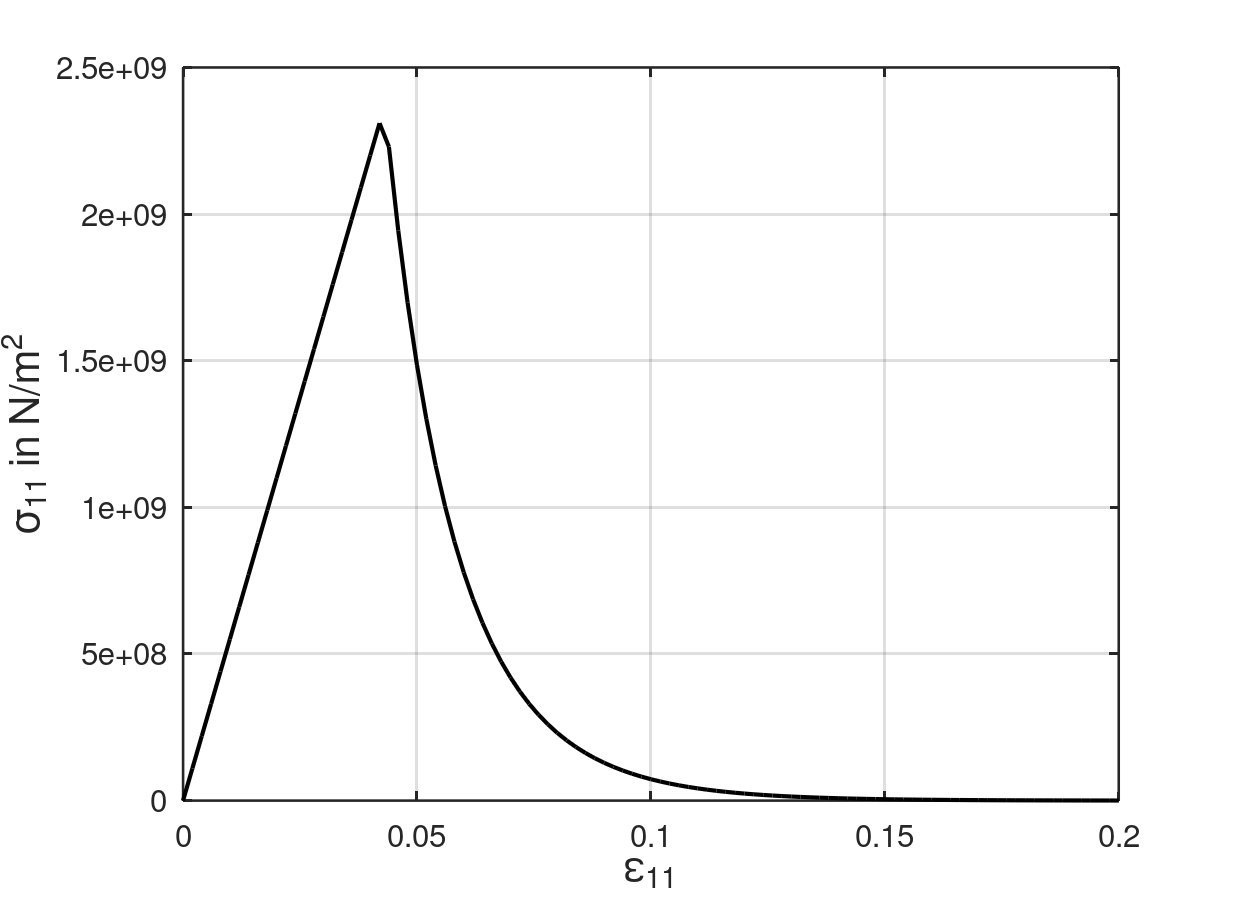
\includegraphics[width=8.3cm,height=8cm,keepaspectratio]{21.StressvsStrain_Ansys.png}
         \caption{Stress-Strain relation (ANSYS)}
         \label{fig:Stress-Strain relation in Ansys}
     \end{subfigure}
     \hspace{1.8cm}
     \begin{subfigure}{0.4\textwidth}
         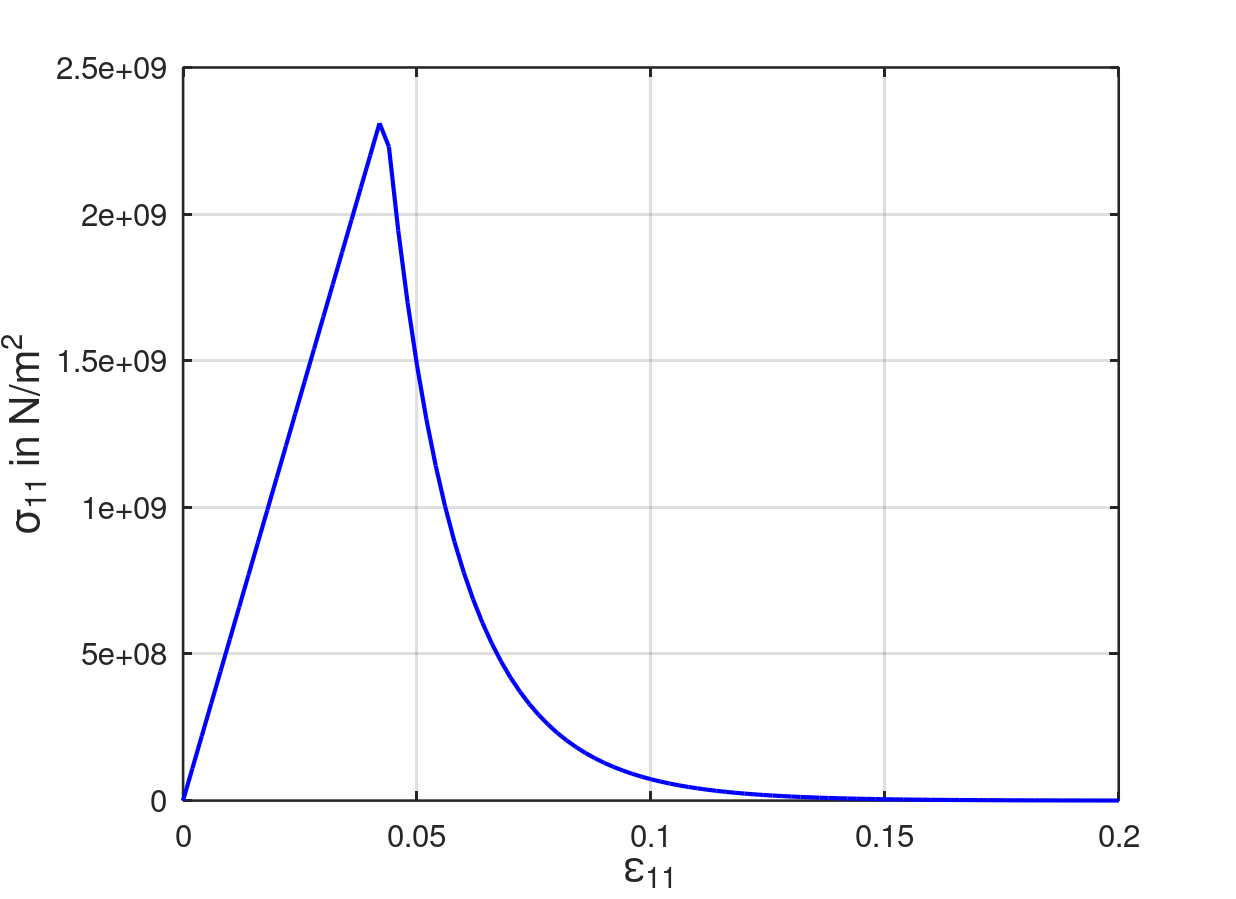
\includegraphics[width=8.3cm,height=8cm,keepaspectratio]{21.StressvsStrain_Octave.png}
         \caption{Stress-Strain relation (Octave)}
         \label{fig:Stress-Strain relation Octave}
     \end{subfigure}
   \caption{Evolution of stress for uniaxial tension test in 11 direction}
   \label{fig:Evolution of stress  component for a uniaxial tension test in 11 direction} 
\end{figure}
\FloatBarrier
\begin{figure}[hbt!]
\begin{center}
  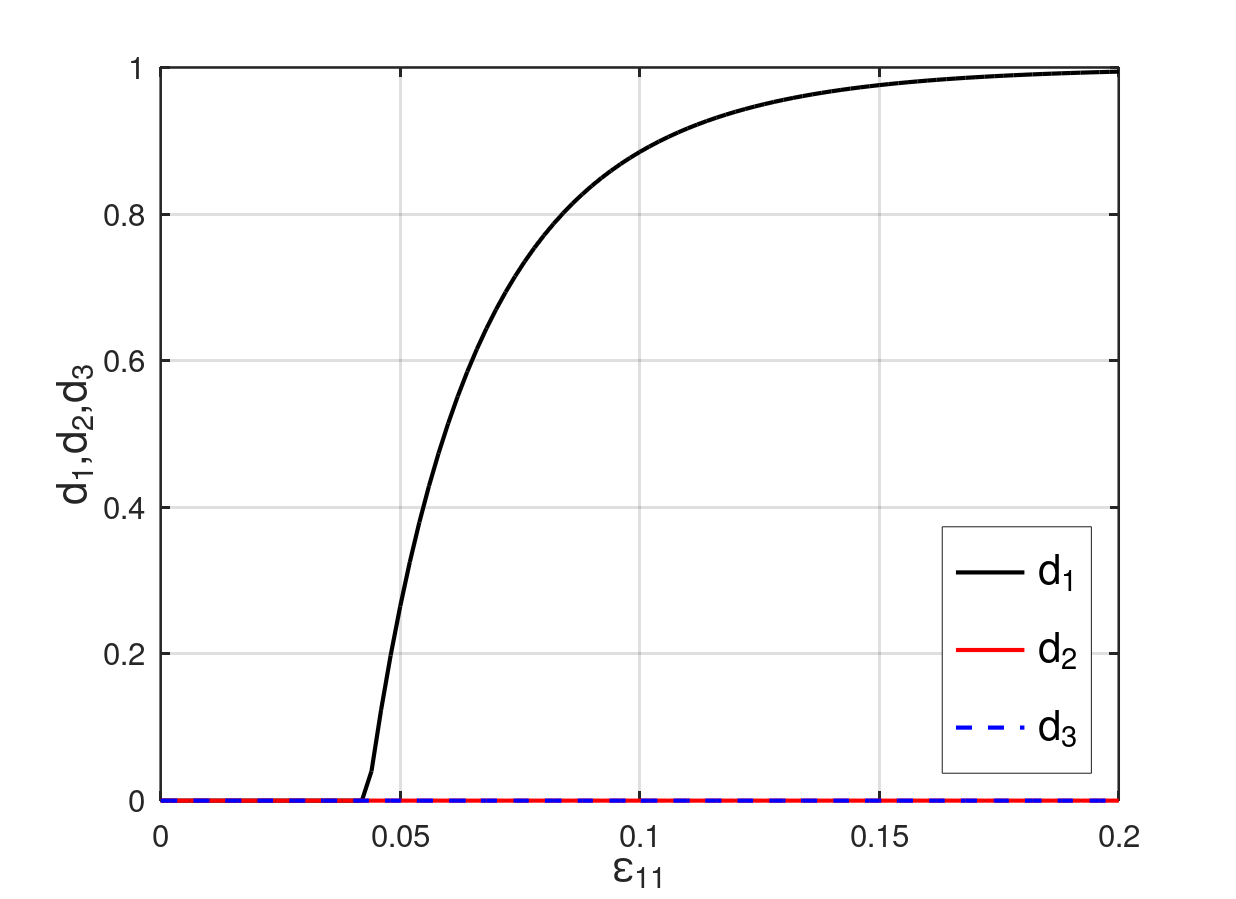
\includegraphics[width=8.6cm,height=8.2cm,keepaspectratio]{21.d1,d2,d3.png}
   \caption{Evolution of damage components for uniaxial tension test in 11 direction}
   \label{fig:Evolution of damage in 11 direction} 
 \end{center}    
\end{figure}
\FloatBarrier
\indent\indent\indent The system is linearly elastic until the damage initiation strain, and the damage is zero. Once the strain $\epsilon_{11}$ exceeds the damage initiation strain, the damage $d_{1}$ starts to evolve exponentially, and the stress starts to drop due to the reduction in stiffness in $1$ direction.  The damage variables $d_{2}$ and $d_{3}$ are zero. The comparison between the figures (\ref{fig:Stress-Strain relation in Ansys}) and (\ref{fig:Stress-Strain relation Octave}) suggests that the material routine implemented in OCTAVE and USERMAT are numerically similar to each other.
The scalar softening parameter ($P$) in the damage evolution equation(\ref{exponential damage equation}) determines the slope of the damage curve. The following figure demonstrates the influence of the softening parameter (P) on the damage evolution
\begin{figure}[hbt!]
\begin{center}
\includegraphics[width=0.7\textwidth]{{21.P_damage.png}}
 \caption{Influence of softening parameter $P$ in the damage evolution)}
 \label{fig:Influence of softening parameter P}
 \end{center}
\end{figure}
\FloatBarrier

\subsubsection{Drawbacks of strain based damage initiation criteria}
\indent\indent\indent Since the lateral contraction is not constrained during uniaxial tension, the transverse directions experience negative strain due to Poisson's effect, i.e., $\epsilon_{22}$ and $\epsilon_{33}$ will be negative. If the compressive strength in the transverse directions 2 and 3 are sufficiently low, the strains  $\epsilon_{22}$ and $\epsilon_{33}$ will exceed the damage initiation strain. This leads to damage evolution without the presence of stress in transverse directions 2 and 3. 
This phenomenon cause convergence issues and the computation stops when the damage evolves without the presence of stress. Figure (\ref{fig:Convergence error}) shows the norm of the residual stress, which does not reach zero (or a tolerance) after 100 iterations of the Newton-raphson, which indicates the failure of the model to converge to a solution when using low compressive strength in the transverse direction ($Y_{c}$ = -180MPa)
\begin{figure}[htbp!]
\begin{center}
\includegraphics[width=0.7\textwidth]{{22.Convergence_error.png}}
 \caption{Convergence issue: Residual norm of the stress $vs$ No of Newton-raphson iterations}
 \label{fig:Convergence error}
 \end{center}
\end{figure}
\FloatBarrier
This problem can be rectified by using stress-based damage initiation criteria. Since damage evolution depends on failure index $F$, the transverse failure indices $F_{m}$ and $F_{z}$ will be zero during uniaxial tension if the stress-based damage initiation criteria are used. This results in zero damage in the transverse direction. The following section presents the results obtained using stress-based damage initiation and the use of mesh regularisation in the damage evolution law.

\subsubsection{Stress based damage initiation and mesh regularisation}
\indent\indent\indent As mentioned in section (\ref{Mesh Regularisation}), the strain localisation problems result in strong mesh dependency, so fracture energy and characteristic length ($L_{c}$) of the element have to be been included in the damage evolution law in order to alleviate the problem. So the material routine is modified by changing the damage initiation criteria to maximum stress criteria (\ref{tab:Maximum stress criterion}) and including the damage evolution equations from (\ref{d1}) to (\ref{d3}). The uniaxial tension is conducted again with the changes mentioned above and with very low transverse compression strength, and the results are presented below.
\begin{figure}[htbp!]
     \captionsetup[subfigure]{justification=centering}
     \begin{subfigure}{0.4\textwidth}
         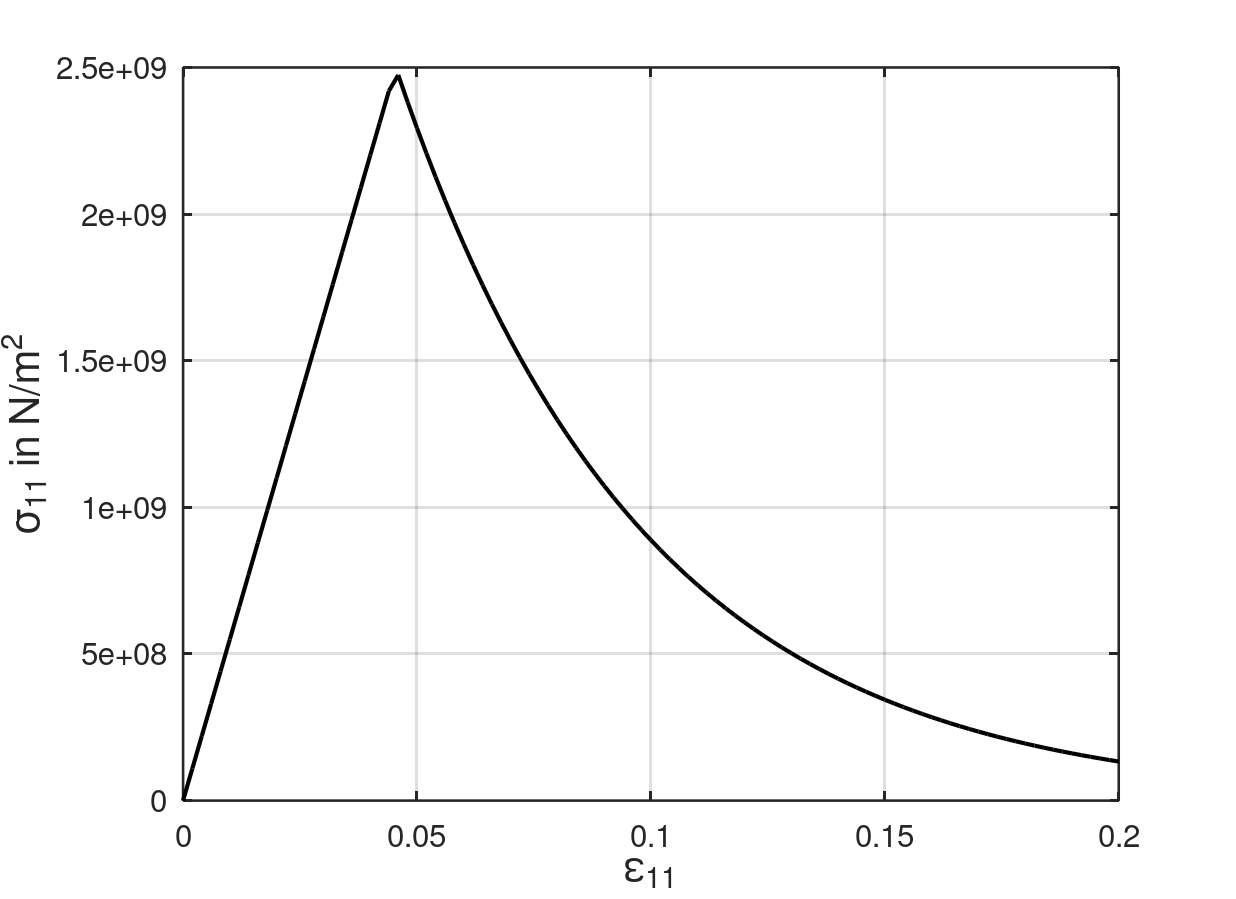
\includegraphics[width=8.3cm,height=8cm,keepaspectratio]{22.StressvsStrain_Ansys.png}
         \caption{Stress-Strain relation (ANSYS)}
         \label{fig:Stress-Strain relation in Ansys2}
     \end{subfigure}
     \hspace{1.8cm}
     \begin{subfigure}{0.4\textwidth}
          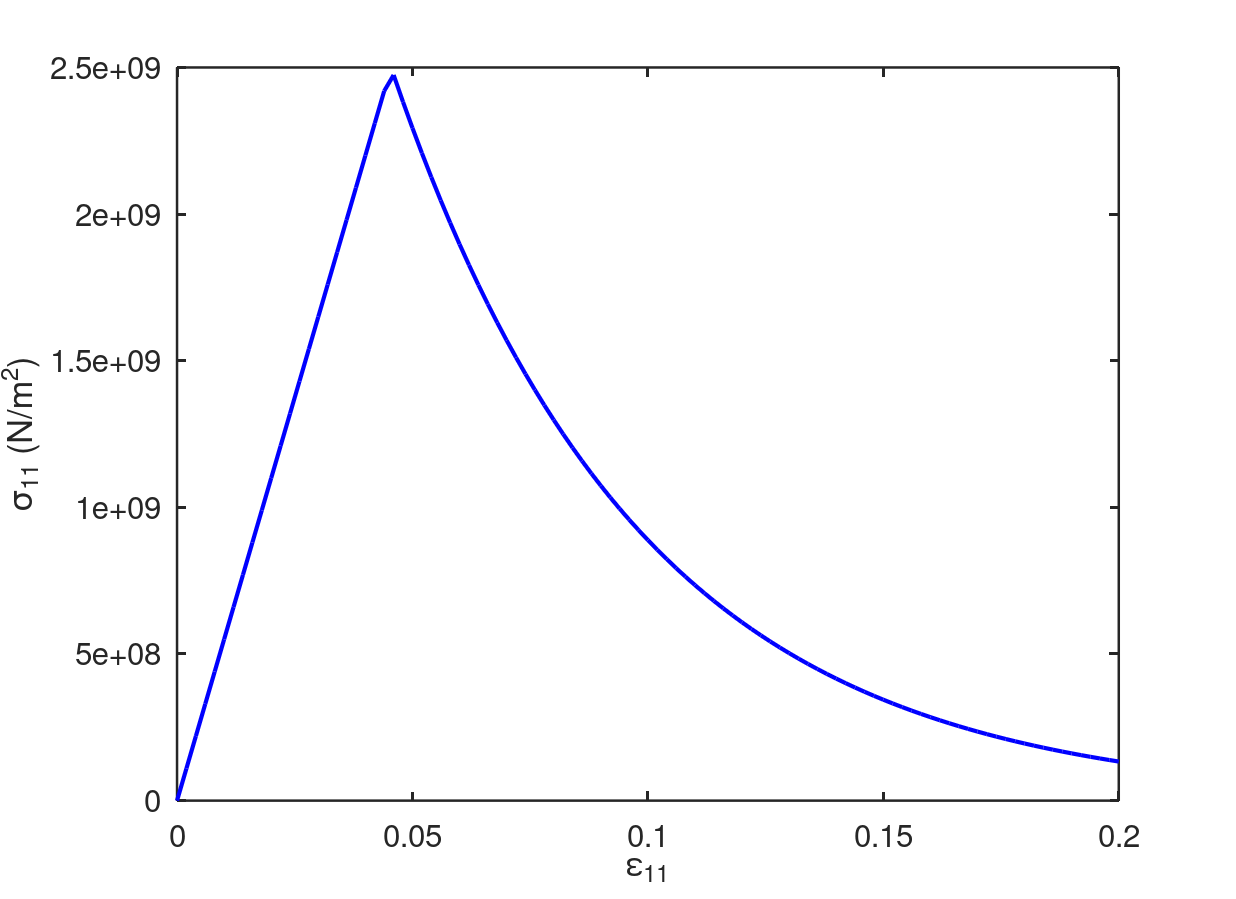
\includegraphics[width=8.3cm,height=8cm,keepaspectratio]{22.StressvsStrain_Octave.png}
         \caption{Stress-Strain relation (Octave)}
         \label{fig:Stress-Strain relation Octave2}
     \end{subfigure}
\end{figure}
\FloatBarrier
\begin{figure}[htbp!]\ContinuedFloat 
	\centering
     \begin{subfigure}{0.4\textwidth}
         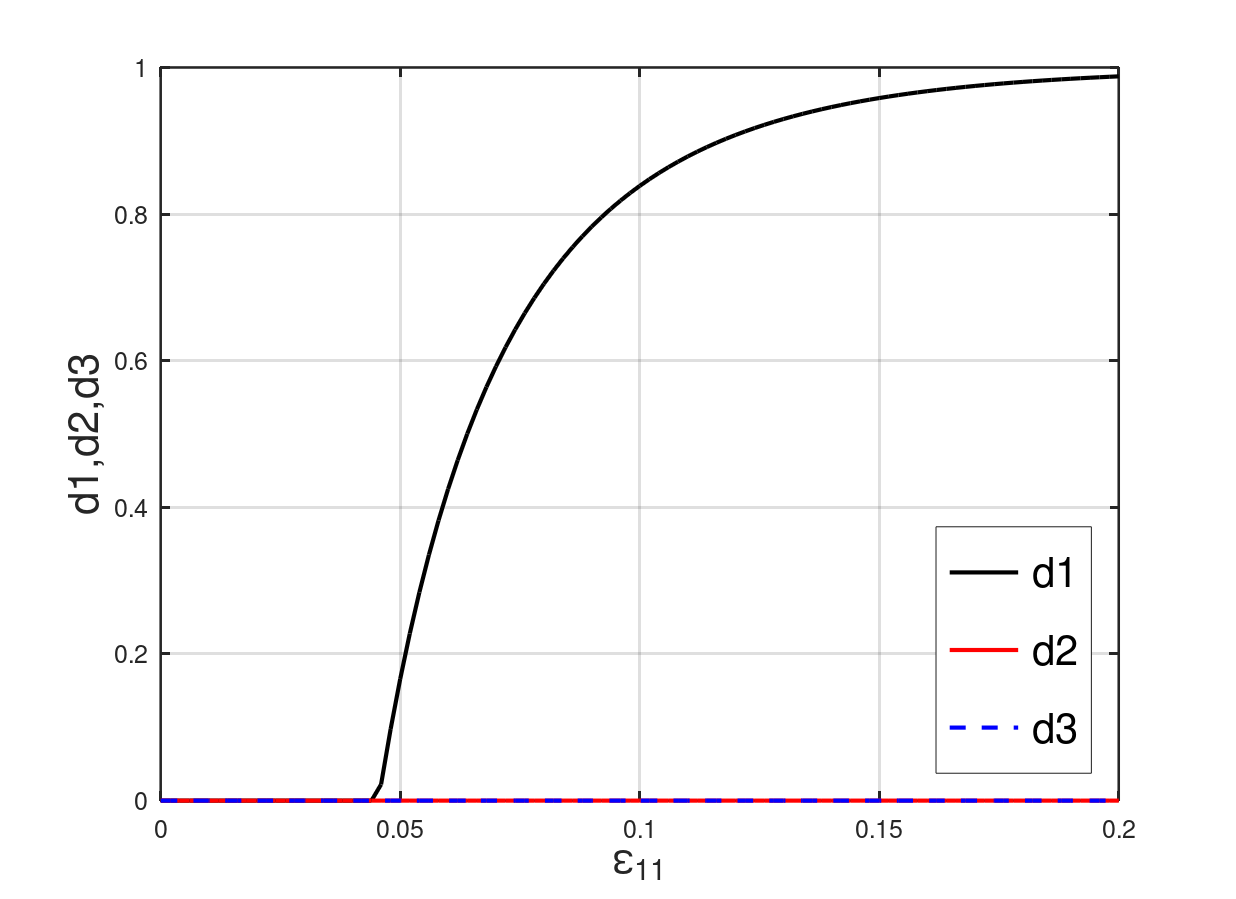
\includegraphics[width=8.6cm,height=8.2cm,keepaspectratio]{22.d1,d2,d3.png}
         \caption{Evolution of damage}
         \label{fig:Evolution of damage in 11 direction2}
     \end{subfigure}
        \caption{Evolution of stress and damage components with stress-based damage initiation criteria under uniaxial tension}
        \label{fig:Evolution of stress and damage components 2}     
\end{figure}
\FloatBarrier
From figure (\ref{fig:Evolution of damage in 11 direction2}) it is evident that the damage  $d_{2}$ and $d_{3}$ are zero as a result of stress-based damage initiation because the stress components $\sigma_{22}$ and $\sigma_{33}$ are zero under uniaxial tension. While using mesh regularisation, the slope of the damage curve is determined by the characteristic length ($L_{c}$), which depends on the volume of the element. The following figure (\ref{fig:Influence of softening parameter P}) shows how the damage evolution is affected by the volume of the element,
\begin{figure}[htbp]
\begin{center}
\includegraphics[width=0.65\textwidth]{{22.V_damage.png}}
 \caption{Influence of element volume ($V$) on the damage evolution}
 \label{fig:Influence of element volume}
 \end{center}
\end{figure}
\FloatBarrier


\subsubsection{Discussion of tangent stiffness}
\indent\indent\indent In the case of uniaxial tension, the components of the stress tensor other than $\sigma_{11}$ are zero. Since stress conditions are enforced, the OCTAVE driver routine uses the Newton-raphson method to determine the input strain components other than $\epsilon_{11}$ iteratively. The Newton-raphson method requires a tangent stiffness for computation which can be derived using the equation (\ref{Anisotropic tangent stiffness}) for anisotropic damage. This enables us to test the derived algorithmic tangent stiffness (ATS) before implementing it in USERMAT. The derived algorithmic tangent stiffness is verified by comparing it with the numerical tangent stiffness computed using numerical perturbation. In numerical perturbation, the coefficients of the strain tensor are perturbed by a very small value, i.e.,  $\Delta\epsilon_{kl}^{n+1} = \delta$ (where $\delta<<1$) and the resulting stress perturbations are calculated. 

\begin{equation}
\Delta\sigma_{ij}^{n+1} \; = \; \sigma_{ij}^{n+1}(\epsilon_{kl}^{n+1}+\delta) - \sigma_{ij}^{n+1}(\epsilon_{kl}^{n+1})
\end{equation}
Then the components of the tangent stiffness tensor can be estimated as
\begin{equation}
 C_T \;  =  \;  \frac{\Delta\sigma_{ij}^{n+1}}{\Delta\epsilon_{kl}^{n+1}}
\end{equation}
Since the material routine must be evaluated for every perturbation of $\epsilon_{kl}$ the routine has to be called six time recursively per load-step iteration. The figure (\ref{fig:Algorithmic tangent})  and (\ref{fig:Numerical perturbation}) shows the strain components $\epsilon_{22}$ and $\epsilon_{33}$ computed using algorithmic and numerical tangent stiffness which are plotted against $\epsilon_{11}$  respectively.
\begin{figure}[htbp!]
     \begin{subfigure}{0.4\textwidth}
         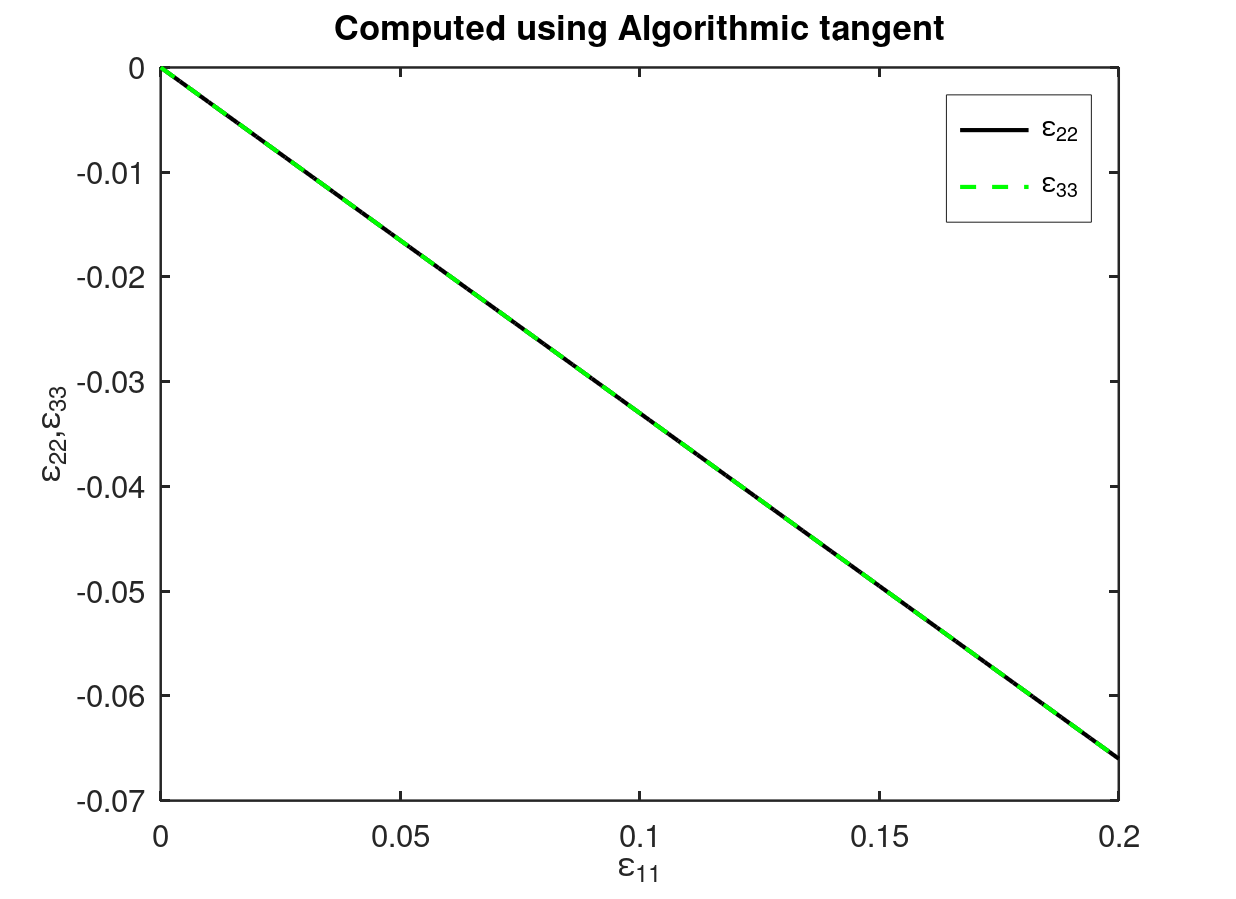
\includegraphics[width=8.3cm,height=8cm,keepaspectratio]{22.e11vse22e33_ATS.png}
         \caption{$\epsilon_{22}, \epsilon_{33}$ vs $\epsilon_{11}$ (Algorithmic tangent)}
         \label{fig:Algorithmic tangent}
     \end{subfigure}  
     \hspace{1.8cm}
     \begin{subfigure}{0.4\textwidth}
         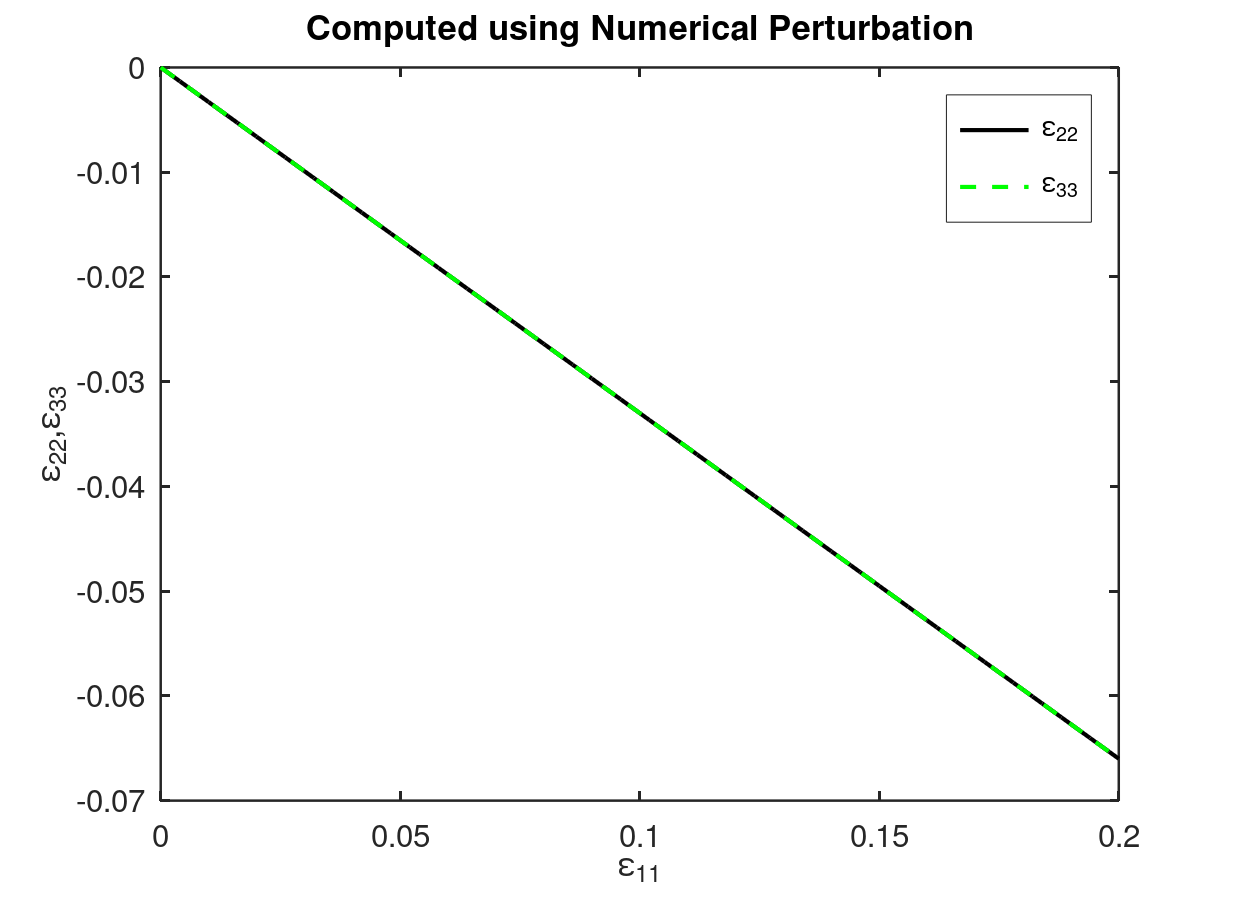
\includegraphics[width=8.3cm,height=8cm,keepaspectratio]{22.e11vse22e33_NT.png}
         \caption{$\epsilon_{22}, \epsilon_{33}$ vs $\epsilon_{11}$ (Numerical perturbation)}
         \label{fig:Numerical perturbation}
     \end{subfigure}
        \caption{The strain components $\epsilon_{22}$ and $\epsilon_{33}$ computed using algorithmic (a) and numerical tangent stiffness (b) under uniaxial tension}
        \label{fig: Algorithmic and numerical tangent stiffness under uniaxial tension}     
\end{figure}
\FloatBarrier
These comparison between above plots clearly indicates that the tangent stiffness computed using algorithmic tangent and numerical tangent are numerically similar to each other.
\subsection{Biaxial tension}
\indent\indent\indent  In the case of biaxial tension, normal stresses are present only in two normal directions, and all the shear stresses are zero as well as the normal stress in third direction, i.e., only two non-zero components presented located on the main diagonal of the stress tensor . In ANSYS, biaxial tension is achieved by applying the same displacements in two normal directions of the finite element ($1$ and $2$ direction), and the contraction in the third direction ($3$) is unconstrained. The following figures show the corresponding stress and damage components obtained from the test.
\begin{figure}[hbt!]
     \captionsetup[subfigure]{justification=centering}
     \begin{subfigure}{0.4\textwidth}
         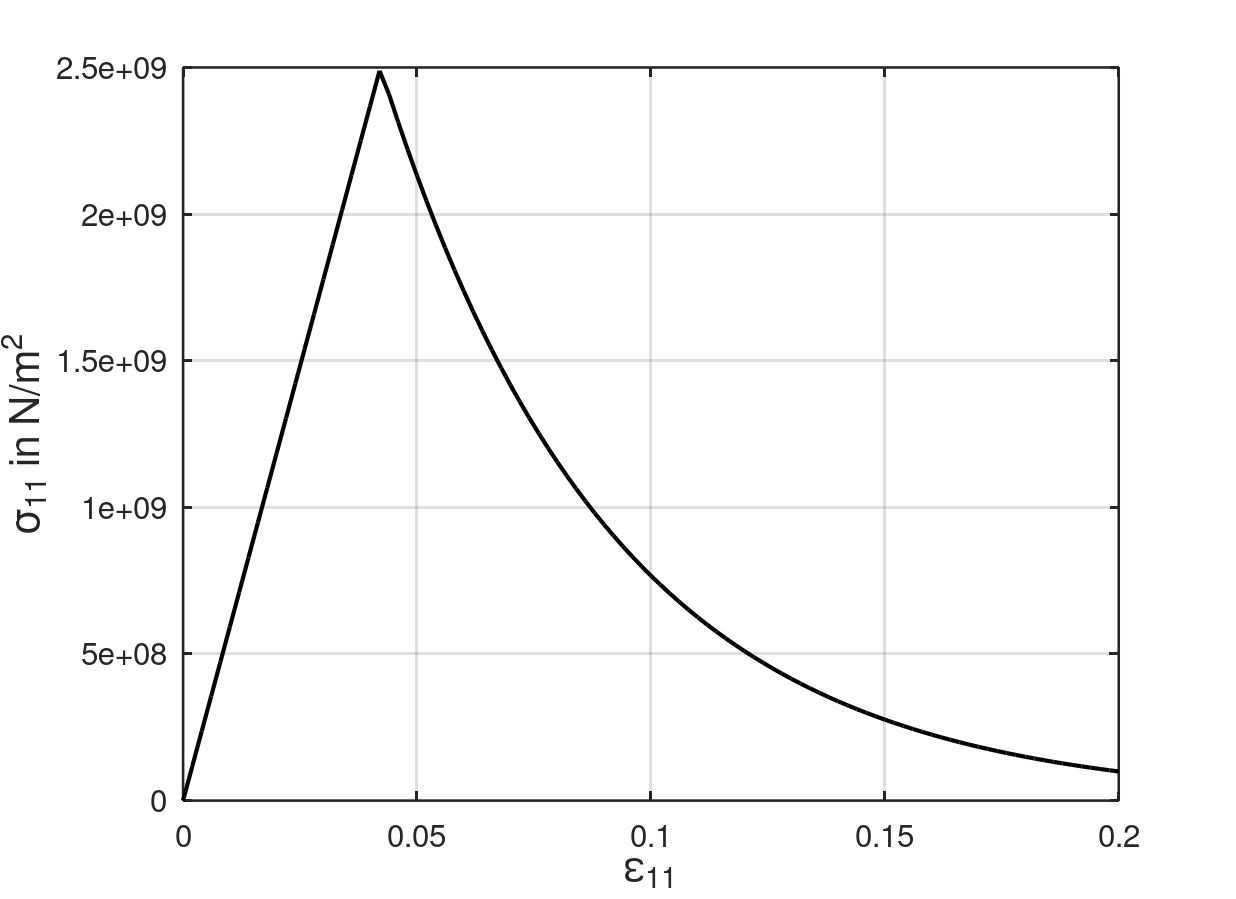
\includegraphics[width=8.3cm,height=8cm,keepaspectratio]{23.S11vsE11.png}
         \caption{$\sigma_{11}$ vs $\epsilon_{11}$}
         \label{fig:S11vsE11}
     \end{subfigure}
	\hspace{1.8cm}
     \captionsetup[subfigure]{justification=centering}
     \begin{subfigure}{0.4\textwidth}
         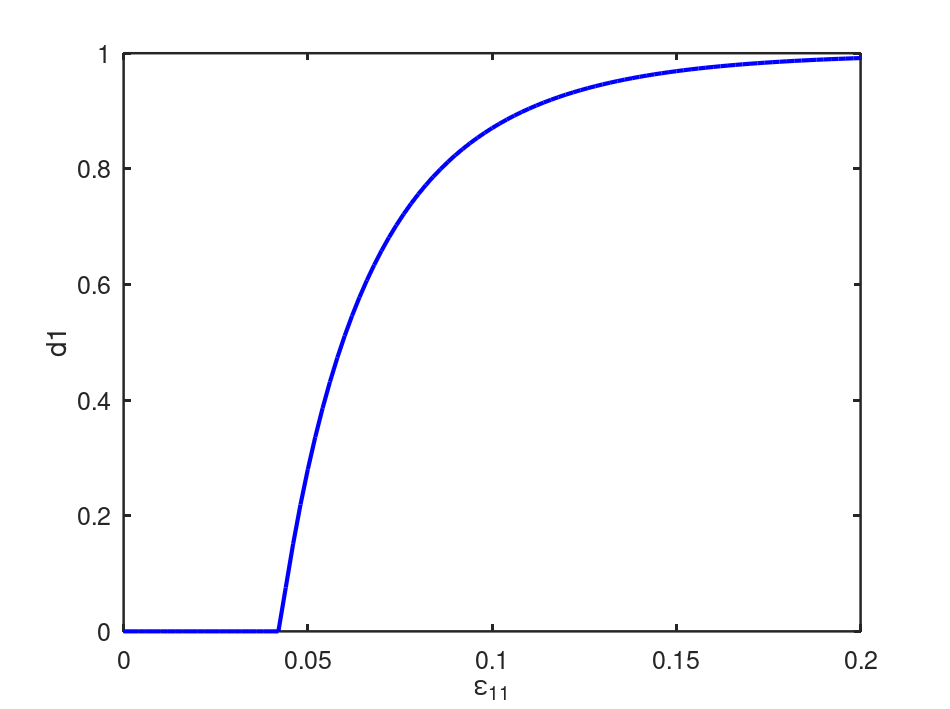
\includegraphics[width=8.3cm,height=8cm,keepaspectratio]{23.d1.png}
         \caption{Evolution of damage $d_{1}$}
         \label{fig:Evolution of damage d1}
     \end{subfigure}
\end{figure}
\FloatBarrier
\begin{figure}[htbp!]\ContinuedFloat 
     \begin{subfigure}{0.4\textwidth}
         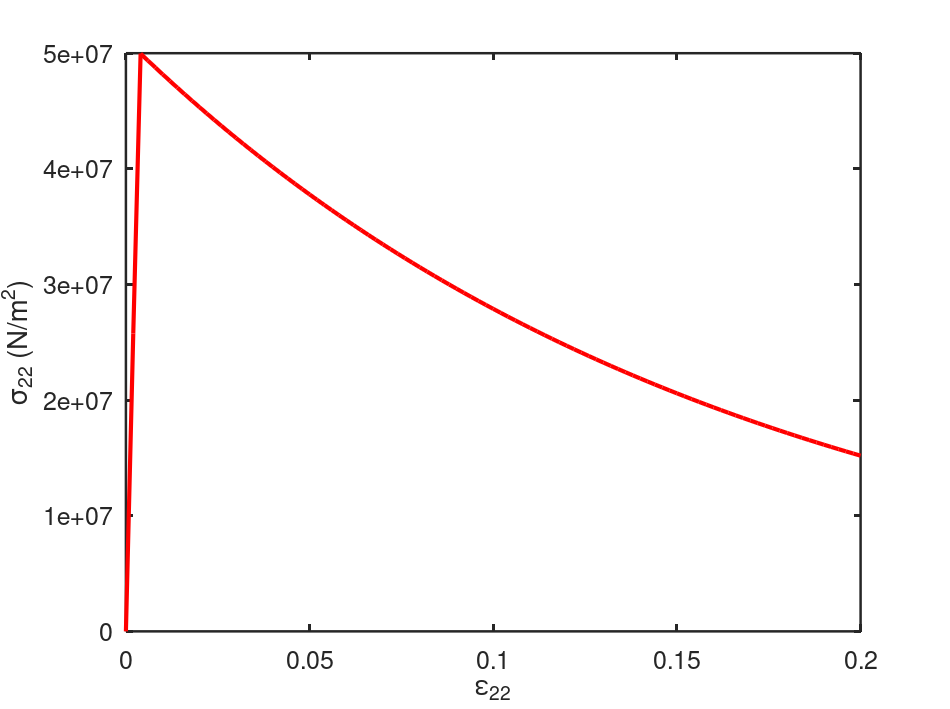
\includegraphics[width=8.3cm,height=8cm,keepaspectratio]{23.S22vsE22.png}
         \caption{$\sigma_{22}$ vs $\epsilon_{22}$}
         \label{fig:S22vsE22}
     \end{subfigure}
     \hspace{1.8cm}
     \begin{subfigure}{0.4\textwidth}
         \centering
         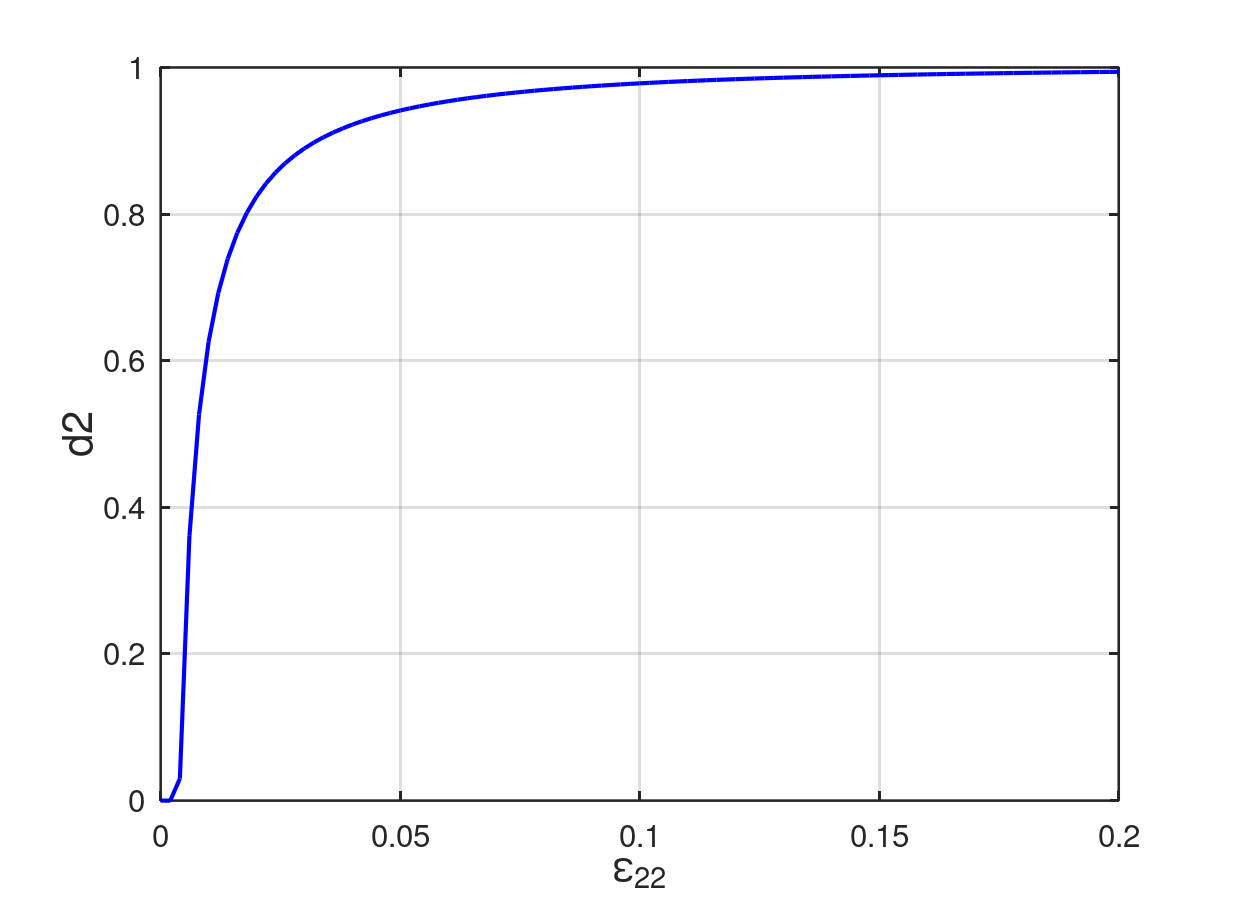
\includegraphics[width=8.3cm,height=8cm,keepaspectratio]{23.d2.png}
         \caption{Evolution of damage $d_{2}$}
         \label{fig:Evolution of damage d2}
     \end{subfigure}
    
        \caption{Evolution of stress (Figures a, c on the left) and corresponding damage (Figure b, d on the right) components under biaxial tension}
        \label{fig:Evolution of damage under biaxial tension}     
\end{figure} 
\FloatBarrier
Since the tensile strength in transverse direction is very low compared to the longitudinal direction, evolution of damage ($d_{2}$) begins very soon and simultaneously the stress component ($\sigma_{22}$) drops as seen in figures (\ref{fig:S22vsE22}) and (\ref{fig:Evolution of damage d2}).


\subsection{Triaxial tension}
\indent\indent\indent In the case of triaxial tension, the normal stresses are present in all three normal directions, and all the shear stresses are zero, i.e., only diagonal components of the stress tensor are non-zero.  In Ansys, triaxial tension is achieved by applying the same displacement in all three normal directions ($1$, $2$ and $3$ direction). The following figures show the corresponding stress and damage components obtained from the test.\\

\begin{figure}[htbp!]
       \captionsetup[subfigure]{justification=centering}
     \begin{subfigure}{0.4\textwidth}
         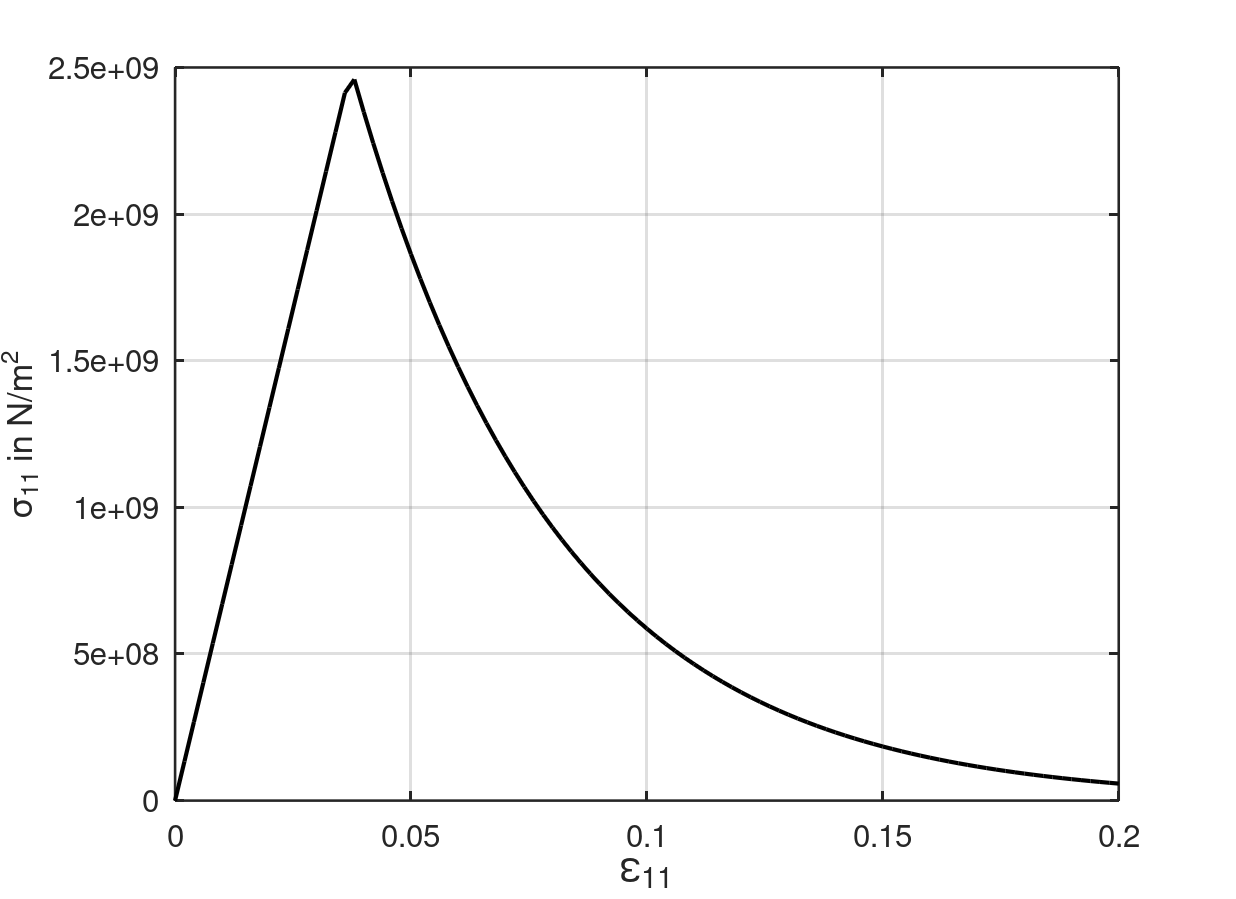
\includegraphics[width=8.3cm,height=8cm,keepaspectratio]{24.S11vsE11.png}
         \caption{$\sigma_{11}$ vs $\epsilon_{11}$}
         \label{fig:S11vsE11 2}
     \end{subfigure}
     \hspace{1.8cm}
     \captionsetup[subfigure]{justification=centering}
     \begin{subfigure}{0.4\textwidth}
         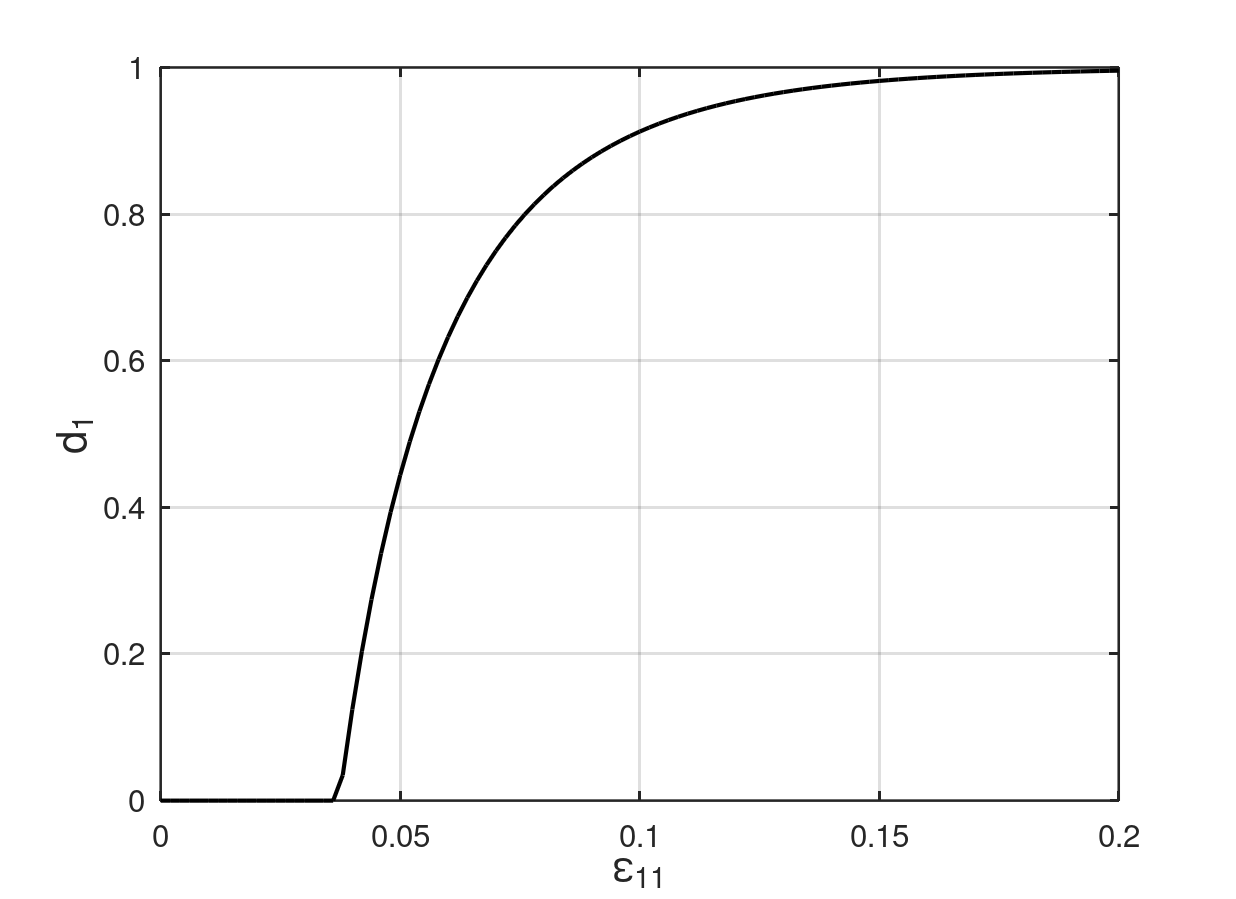
\includegraphics[width=8.3cm,height=8cm,keepaspectratio]{24.d1.png}
         \caption{Evolution of damage $d_{1}$}
         \label{fig:Evolution of damage d1 2}
     \end{subfigure}
\end{figure}
\FloatBarrier
\begin{figure}[htbp!]\ContinuedFloat 
     \begin{subfigure}{0.4\textwidth}
         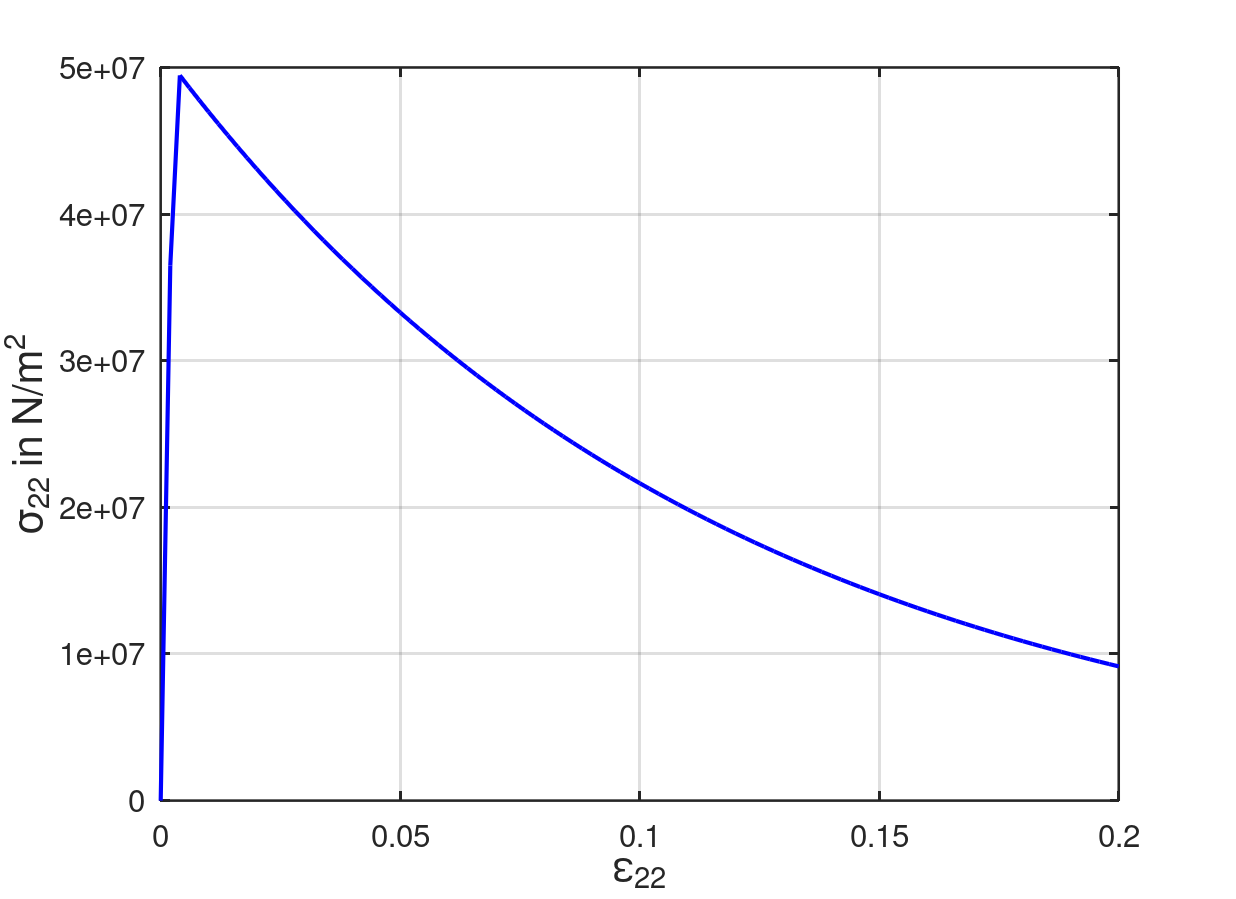
\includegraphics[width=8.3cm,height=8cm,keepaspectratio]{24.S22vsE22.png}
         \caption{$\sigma_{22}$ vs $\epsilon_{22}$}
         \label{fig:S22vsE22 2}
     \end{subfigure}   
     \hspace{1.8cm}
     \begin{subfigure}{0.4\textwidth}
         \centering
         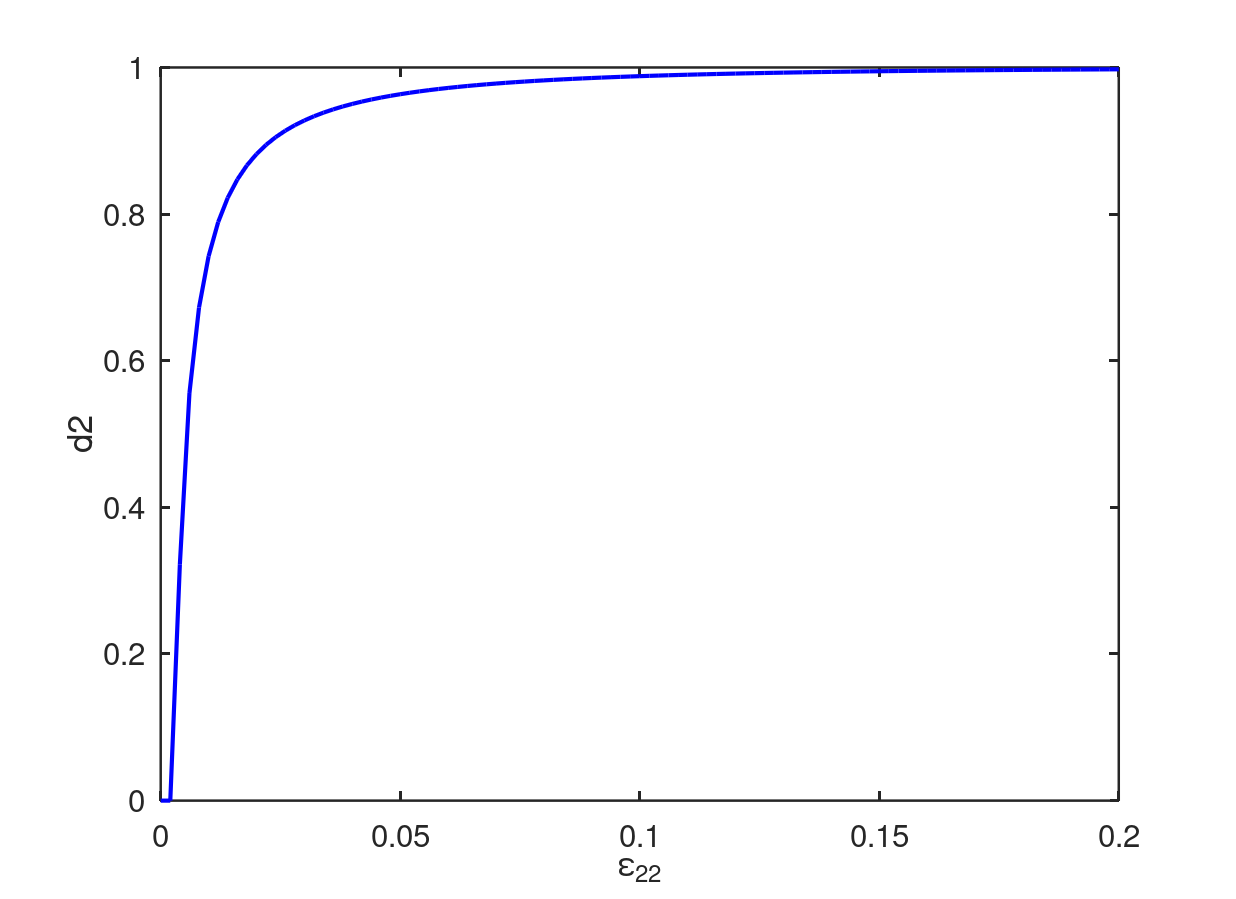
\includegraphics[width=8.3cm,height=8cm,keepaspectratio]{24.d2.png}
         \caption{Evolution of damage $d_{2}$}
         \label{fig:Evolution of damage d2 2}
     \end{subfigure}
\end{figure}
\FloatBarrier
\begin{figure}[htbp!]\ContinuedFloat
     \begin{subfigure}{0.4\textwidth}
         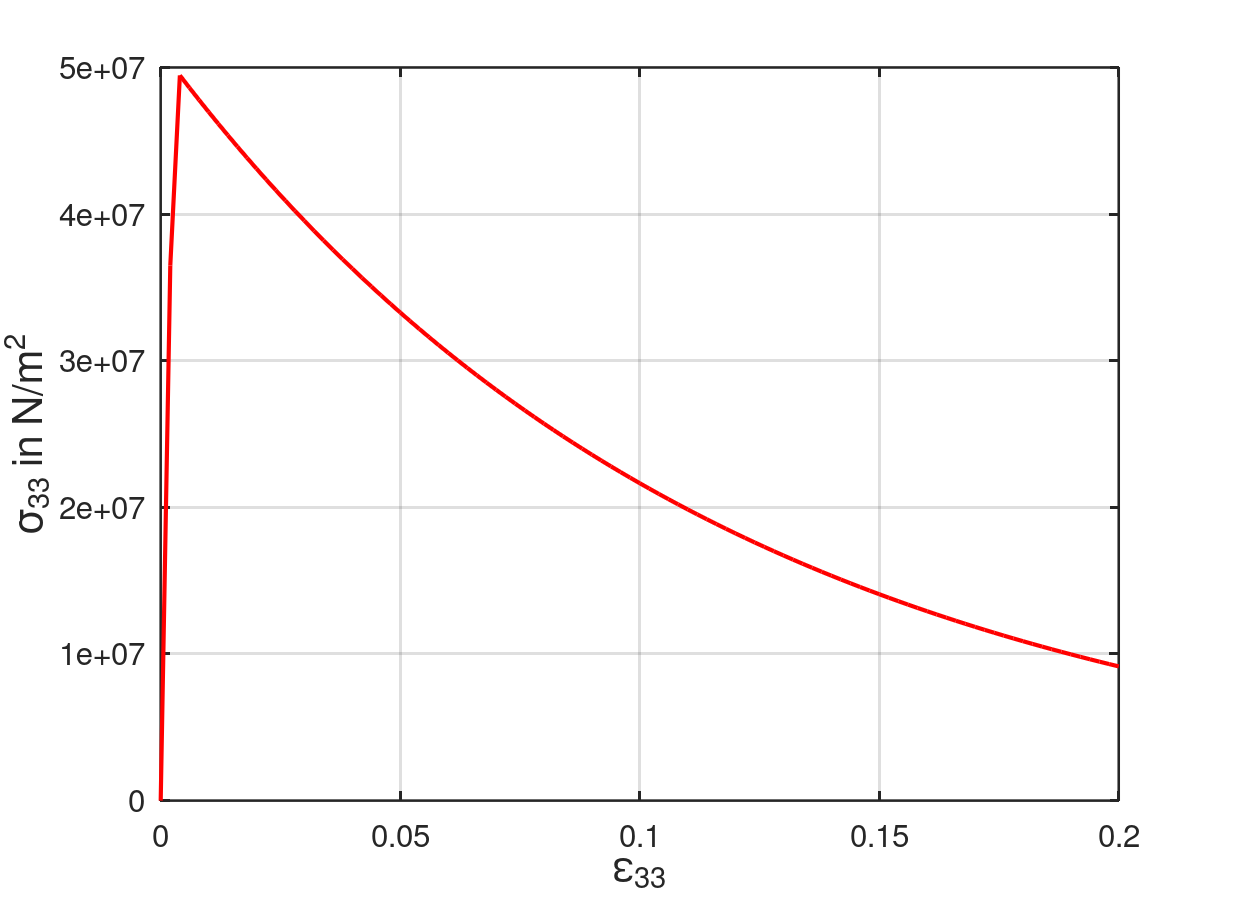
\includegraphics[width=8.3cm,height=8cm,keepaspectratio]{24.S33vsE33.png}
         \caption{$\sigma_{33}$ vs $\epsilon_{33}$}
         \label{fig:S33vsE33}
     \end{subfigure}
     \hspace{1.8cm}
     \begin{subfigure}{0.4\textwidth}
         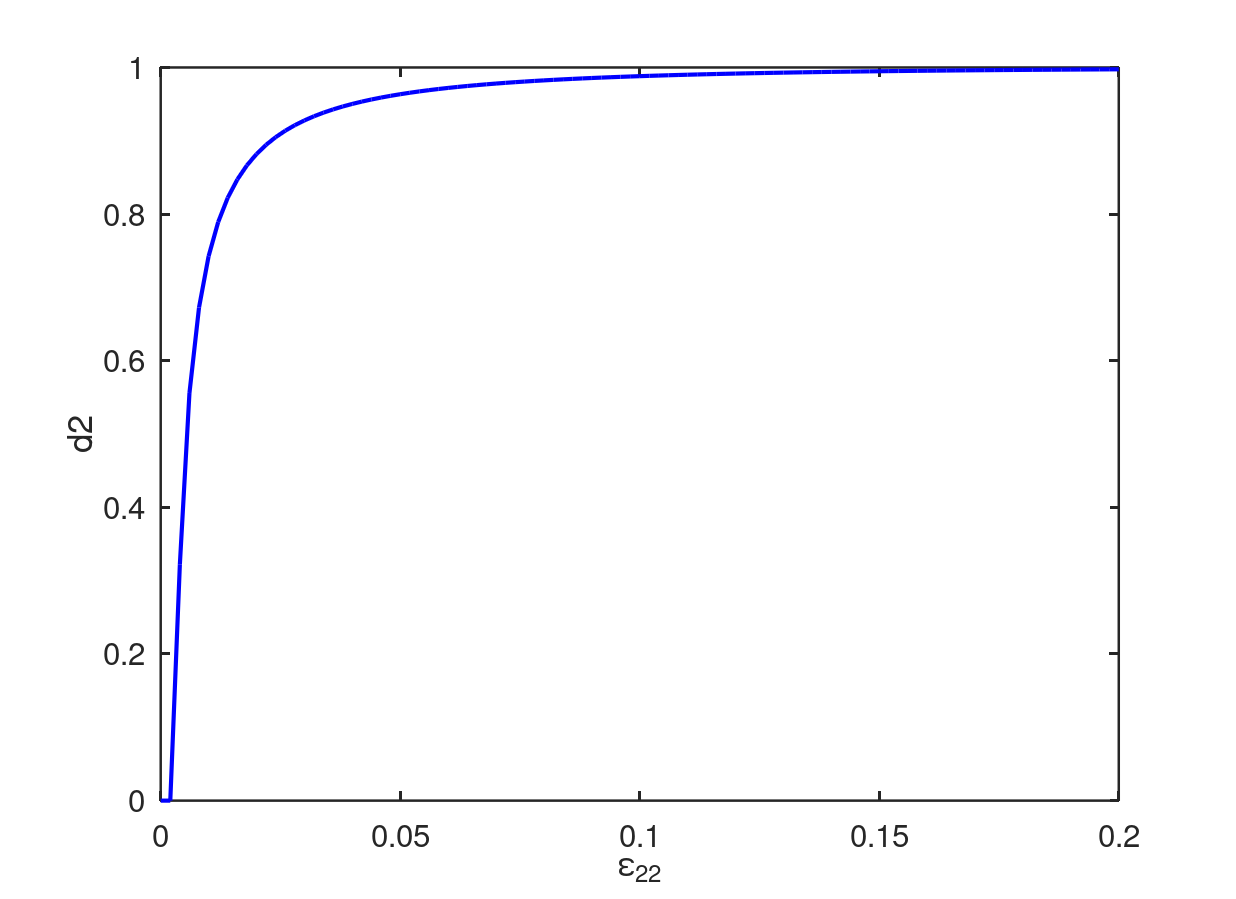
\includegraphics[width=8.3cm,height=8cm,keepaspectratio]{24.d2.png}
         \caption{Evolution of damage $d_{3}$}
         \label{fig:Evolution of damage d3}
     \end{subfigure}     
        \caption{Evolution of stress (Figures a, c, e on the left) and corresponding (Figures b ,d, f on the right) damage components under triaxial tension}
        \label{fig:Evolution of damage under triaxial tension}     
\end{figure}
\FloatBarrier
Since the material properties are the same in transverse $2$ and $3$ direction and the tensile strength is very low compared to the longitudinal $1$ direction, the damage $d_{2}$ and $d_{3}$ evolves simultaneously (Figure (\ref{fig:Evolution of damage d2 2}) and (\ref{fig:Evolution of damage d3})) and very soon as expected. Therefore the stress components $\sigma_{22}$ and $\sigma_{33}$ drop very soon as shown in Figure (\ref{fig:S22vsE22 2}) and (\ref{fig:S33vsE33}) 
\section{Representative structural examples}
\indent\indent\indent The following structural examples are used to test the damage model implemented as a USERMAT in the ANSYS environment
\begin{itemize}
\item Notched tensile specimen (2D - Plane stress)
\item Compact tension (CT) specimen (2D - Plane stress)
\item Plate with hole (3D)
\end{itemize}
Each example is chosen to demonstrate specific features of the damage model. These features include, at first, the capability of the model to represent damage initiation and propagation and secondly, the calculation of multiple damage variables, i.e., the ability to show anisotropic damage development in the composite material when a load is applied, both in 2D and 3D setting. Furthermore, mesh convergence studies are performed to show that the regularization scheme employed gives better results than the model with no regularization. For all the finite element simulations of the above models, linear quadrilateral elements are used (both 2D and 3D) with full Gauss integration. The line search option has been enabled during all the simulations to get good convergence behaviour. The material used for the finite element simulations is T700/2510 carbon fiber/epoxy fabric. The material has fibers in parallel in the longitudinal direction and fibers woven in the cross-section that provide additional strength in transverse directions. The material has a high modulus and strength in the longitudinal direction because of the presence of a large number of fibers. The material properties are obtained from  and a summary of the material properties are given in the Table (\ref{tab:Material parameters(Representative structural examples)}). \\
\begin{table}[!htbp]
  \begin{center}
     \resizebox{\columnwidth}{5.8cm}{
     \begin{tabular}{l l l} 
     \hline
     \\
      \textbf{Symbol} \;\;& \textbf{Material Parameter} \;& \textbf{Value}\\
      \\
      \hline
      \\
      \vspace*{0.1cm}
      $E_{11}$ & Modulus in longitudinal (1) direction &  55.8 GPa\\
      \vspace*{0.1cm}
      $E_{22}$ = $E_{33}$  & Modulus in transverse (2 and 3) directions   & 54.9 GPa \\
      \vspace*{0.1cm}
      $\nu_{12}$ & Poisson's ratio   & 0.043 \\
      \vspace*{0.1cm}
      $G_{12}$ =  $G_{23}$ = $G_{13}$   &  Shear modulus  & 4.2 GPa \\
      \vspace*{0.1cm}
      $X_{t}$ &  Tensile strength in longitudinal (1) direction & 910.1 MPa\\
      \vspace*{0.1cm}
      $X_{c}$ & Compressive strength in longitudinal (1) direction & -710.2 MPa\\
      \vspace*{0.1cm}
      $Y_{t}$ & Tensile strength in (2 and 3) directions  & 772.2 MPa\\
      \vspace*{0.1cm}
      $Y_{c}$ & Compressive strength in (2 and 3) directions &  -703.3 MPa\\
      \vspace*{0.1cm}
      $S_{12}$ & In-plane strength &  131 MPa\\
      \vspace*{0.1cm}
      $G_{f}^{lt}$ & Tensile fracture energy along longitudinal (1) direction  &  125 KJ/$m^{2}$\\
      \vspace*{0.1cm}
      $G_{f}^{lc}$ & Compressive fracture energy along longitudinal (1) direction  &  250 KJ/$m^{2}$\\
      \vspace*{0.1cm}
      $G_{f}^{tt}$ & Tensile fracture energy along (2 and 3) directions   &  95 KJ/$m^{2}$\\
      \vspace*{0.1cm}
      $G_{f}^{tc}$ & Compressive fracture energy along (2 and 3) directions  & 254 KJ/$m^{2}$\\
      \\
       \hline
    \end{tabular}
    }
    \\
    \caption{Material parameters (Representative structural examples)}
    \label{tab:Material parameters(Representative structural examples)}
  \end{center}
\end{table}
\FloatBarrier
\subsection{Notched tensile specimen}
\indent\indent\indent  The first example demonstrates the model's capability to represent damage initiation and propagation. A notched tensile specimen is widely used for analysis of stress concentration, fatigue etc., Because of the symmetry, only one-quarter of the specimen is modelled in the finite element analysis and the geometry and boundary conditions are shown in the Figure (\ref{fig:NT Specimen}). The meshes consist of plane-stress elements (PLANE 182) with bilinear interpolations for displacements, and 2*2 Gauss integration has been utilized. Three different finite element meshes have been used in the fracture zone with the elements of h=1 mm, 0.5 mm, 0.25 mm and a total of 500, 840, 1460 elements respectively for the convergence studies (Figure \ref{fig:Considered meshes}).  At first, the longitudinal direction is kept parallel to the loading direction, and the behaviour of the model is analyzed by applying a displacement controlled load ($U_{x}$) in the longitudinal direction (X-direction). The maximum stress criterion (Section \ref{Maximum stress criteria}) has been used to predict the damage initiation.

\begin{figure}[htbp!]
\begin{center}
\includegraphics[width=0.6\textwidth]{{25.Geometry.jpg}}
 \caption{Specimen geometry and boundary conditions. Dimensions are given in mm. Displacement controlled loading $U_{x}$ is applied.}
 \label{fig:NT Specimen}
 \end{center}
\end{figure}
\FloatBarrier
\indent\indent\indent   The force-displacement response for the three different meshes with and without the regularization (Section(\ref{Mesh Regularisation})) schemes have been plotted in Figure (\ref{fig:with regularization})  and (\ref{fig:without regularization}) respectively. The global force-displacement response is characterized by a large linear regime followed by a gradual drop of the load (because of the softening) or a sudden drop in case of no regularization. From Figure (\ref{fig:Convergence study}), it is clearly evident that the model with regularization gives a more stable force-displacement response compared to the model without regularization, where the maximum load capacity is very low, and the load drops significantly with the decrease in mesh size (i.e., increase in the number of elements). Even though the regularization scheme does not fully alleviate the mesh dependency, it improves the solution significantly compared to the material model without regularization. 

\begin{figure}[htbp!]
     \captionsetup[subfigure]{justification=centering}
     \begin{subfigure}{0.27\textwidth}
         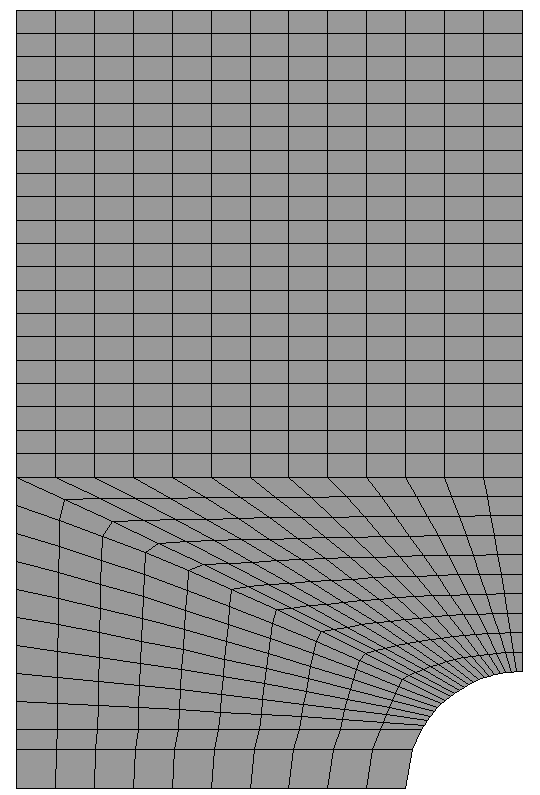
\includegraphics[width=1.15\textwidth]{25.1mm2.png}
         \caption{h=1 mm, n=500 elements}
         \label{fig:1mm}
     \end{subfigure}
     \hfill
     \begin{subfigure}{0.27\textwidth}
         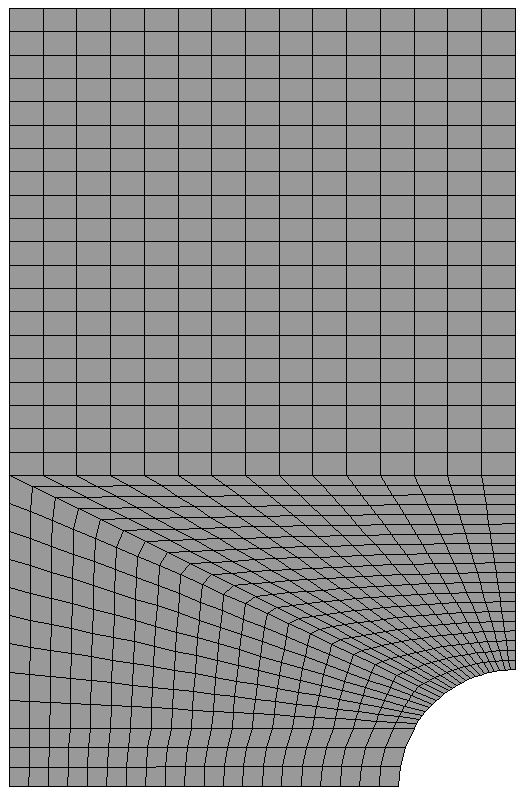
\includegraphics[width=1.27\textwidth]{25.0.5mm2.png}
         \caption{h=0.5 mm, n=840 elements}
         \label{fig:0.5mm}
     \end{subfigure}
     \hfill
     \begin{subfigure}{0.27\textwidth}
         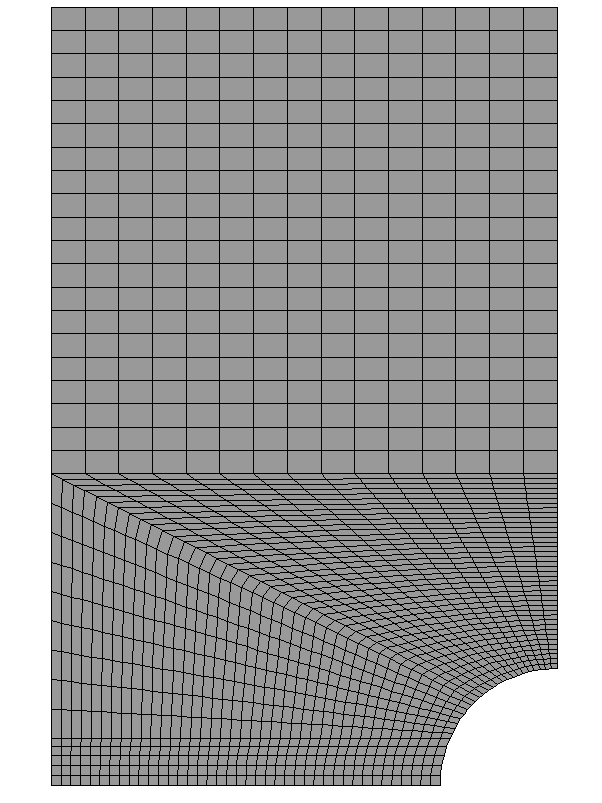
\includegraphics[width=1.27\textwidth]{25.0.25mm2.png}
         \caption{h=0.25 mm, n=1460 elements}
         \label{fig:0.25mm}
     \end{subfigure}
    \caption{Considered meshes (h is the length of the element along fracture zone and n the total number of elements) }
    \label{fig:Considered meshes}
\end{figure}
\FloatBarrier
\begin{figure}[htbp!]
     \captionsetup[subfigure]{justification=centering}
     \begin{subfigure}{0.4\textwidth}
         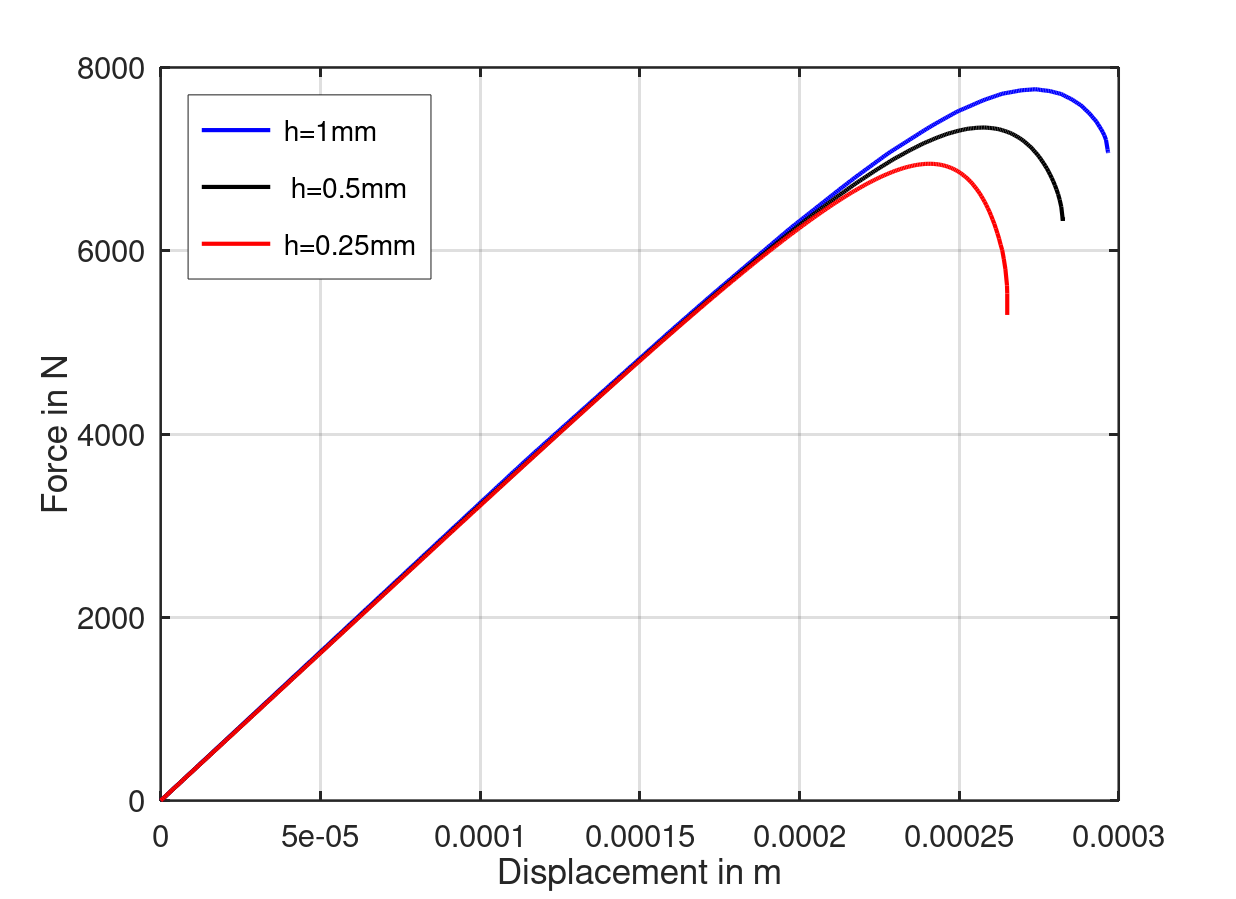
\includegraphics[width=8.2cm,height=7.2cm,keepaspectratio]{25.FvsD.png}
         \caption{model with regularization}
         \label{fig:with regularization}
     \end{subfigure}
     \hspace{1.8cm}
     \begin{subfigure}{0.4\textwidth}
         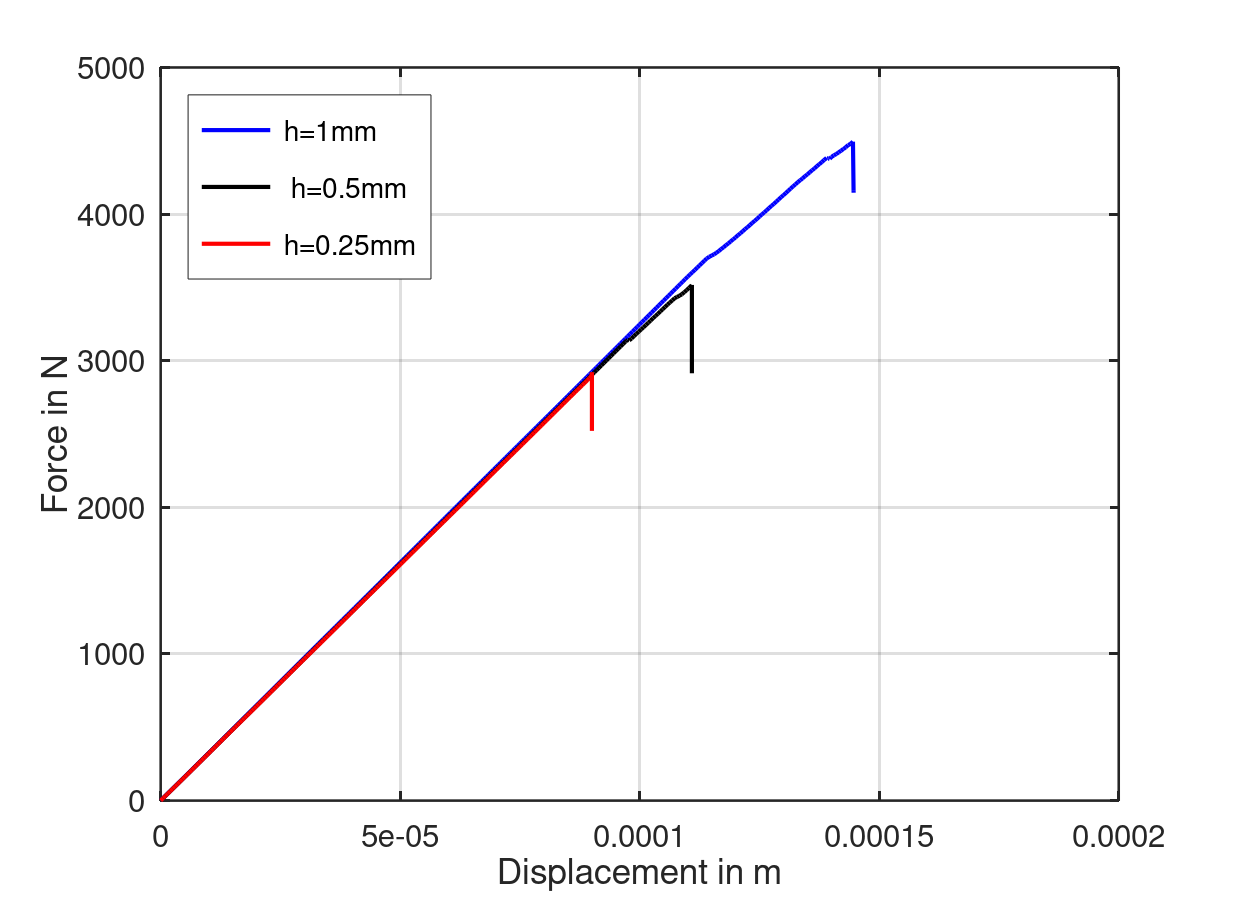
\includegraphics[width=8.2cm,height=7.2cm,keepaspectratio]{25.FvsD2.png}
         \caption{model without regularization}
         \label{fig:without regularization}
     \end{subfigure}
    \caption{Convergence study: Global force-displacement response for model with regularization (Figure a on the left) and without regularization (Figure b the right) }
    \label{fig:Convergence study}
\end{figure}
\FloatBarrier
 
\indent\indent\indent The damage distributions at the end of the process have been plotted for the three different meshes in the Figure (\ref{fig:Convergence study for model with and without regularization}). For numerical reasons the maximum damage is limited to a threshold value of $d_{max}$ = 0.999. The improvement in the global response by using regularization schemes has been illustrated by the damage distributions at the end of the loading process. A relatively large portion of the fracture zone takes part in the damage process instead of very few elements (one or two elements) in the case of no regularization. Damage initiates at the tip of the blunt notch and propagates perpendicular to the loading direction. The width of the damage zone is approximately the same in the three discretizations, but the number of elements that reach a critical damage value (red) increases with the increase in the number of elements along the fracture zone.

\begin{figure}[htbp!]
     \begin{subfigure}{0.4\textwidth}
         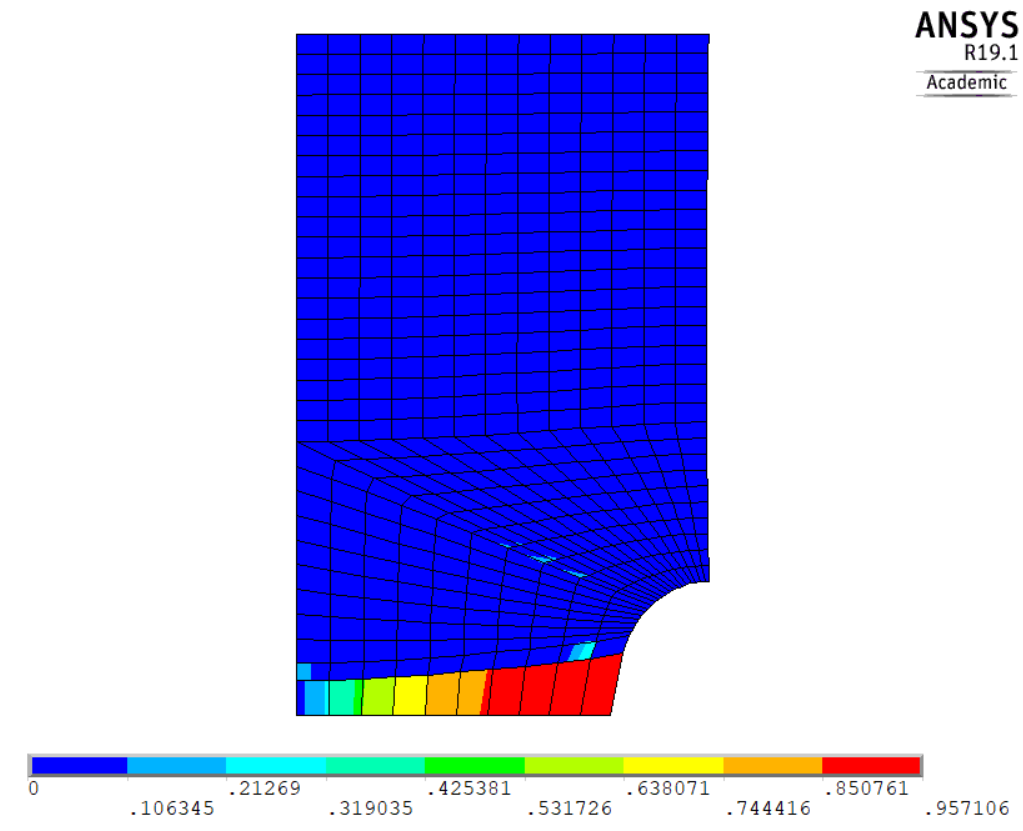
\includegraphics[width=8cm,height=7.2cm,keepaspectratio]{25.d1-1-r.png}
         \caption{h = 1 mm}
         \label{fig:d1-1-r}
     \end{subfigure}
    \hspace{1.8cm}
     \captionsetup[subfigure]{justification=centering}
     \begin{subfigure}{0.4\textwidth}
         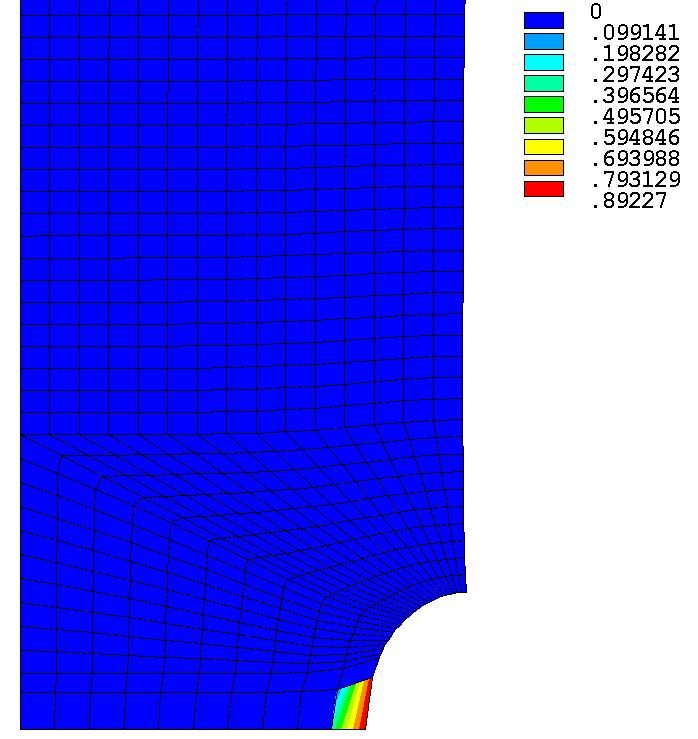
\includegraphics[width=8cm,height=7.2cm,keepaspectratio]{25.d1-1-nr.png}
         \caption{h = 1 mm}
         \label{fig:d1-1-nr}
     \end{subfigure}
\end{figure}
\FloatBarrier
\begin{figure}[htbp!]\ContinuedFloat 
     \begin{subfigure}{0.4\textwidth}
         \includegraphics[width=8cm,height=7.2cm,keepaspectratio]{25.d1-0.5-r.png}
         \caption{h = 0.5 mm}
         \label{fig:d1-0.5-r}
     \end{subfigure}   
     \hspace{1.8cm}
     \begin{subfigure}{0.4\textwidth}
         \includegraphics[width=8cm,height=7.2cm,keepaspectratio]{25.d1-0.5-nr.png}
         \caption{h = 0.5 mm}
         \label{fig:d1-0.5-nr}
     \end{subfigure}
\end{figure}
\FloatBarrier
\begin{figure}[htbp!]\ContinuedFloat
     \begin{subfigure}{0.4\textwidth}
         \includegraphics[width=8cm,height=7.2cm,keepaspectratio]{25.d1-0.25-r.png}
         \caption{h = 0.25 mm}
         \label{fig:d1-0.25-r}
     \end{subfigure}
     \hspace{1.8cm}
     \begin{subfigure}{0.4\textwidth}
         \includegraphics[width=8cm,height=7.2cm,keepaspectratio]{25.d1-0.25-nr.png}
         \caption{h = 0.25 mm}
         \label{fig:d1-0.25-nr}
     \end{subfigure}     
        \caption{Convergence study for model with(Figure a,c,e) and without(b,d,f) regularization: Damage contour plots $d_{1}$ at the end of the loading}
        \label{fig:Convergence study for model with and without regularization}     
\end{figure}
\FloatBarrier
Now the transverse direction is kept parallel to the loading direction, and the behaviour of the damage model, i.e., initiation and propagation of damage $d_{2}$, is analysed by applying a tensile load in the transverse direction. The damage ($d_{2}$) at the end of the loading process is shown in the Figure (\ref{fig:Damage contour plots d2})
\\
\begin{figure}[htbp!]
 \centering
     \captionsetup[subfigure]{justification=centering}
     \begin{subfigure}{0.4\textwidth}
      \centering
         \includegraphics[width=8cm,height=7.2cm,keepaspectratio]{25.d2-1.png}
         \caption{h=1mm}
         \label{fig:d2-1}
     \end{subfigure}
     \hspace{1.8cm}
     \begin{subfigure}{0.4\textwidth}
      \centering
         \includegraphics[width=8cm,height=7.2cm,keepaspectratio]{25.d2-0.5.png}
         \caption{h=0.5mm}
         \label{fig:d2-0.5}
     \end{subfigure}
\end{figure}
\begin{figure}[htbp!]\ContinuedFloat
     \centering
     \begin{subfigure}{0.5\textwidth}
        \centering
        \includegraphics[width=8cm,height=7.2cm,keepaspectratio]{25.d2-0.25.png}
         \caption{h=0.25mm}
         \label{fig:d2-0.25}
     \end{subfigure}
    \caption{Damage contour plots $d_{2}$ at the end of the loading (Loading in transverse direction) }
    \label{fig:Damage contour plots d2}
\end{figure}
\FloatBarrier
The damage pattern looks similar to the distribution of damage ($d_{1}$) when loaded in the longitudinal direction. The force-displacement response of both longitudinal and transverse loading for a single mesh type (h = 0.5mm) is compared in the Figure (\ref{fig:Strength}). As expected, the maximum load capacity is high in the longitudinal direction compared to the transverse direction.

\begin{figure}[htbp!]
\begin{center}
\includegraphics[width=0.7\textwidth]{{25.Strength.png}}
 \caption{Comparison of force-displacement response in longitudinal and transverse direction for h=0.5mm discretization}
 \label{fig:Strength}
 \end{center}
\end{figure}
\FloatBarrier 
 
\subsection{Compact Tension (CT) Specimen}
\indent\indent\indent   This second example demonstrates the model's ability to compute multiple damage variables simultaneously, i.e., show the anisotropic damage development when a load is applied. In the plane stress (2D) setting, two damage variables ($d_{1}$ and $d_{2}$), one in each principal direction, are employed to represent the anisotropic damage development. The Compact Tension test is a standard test for plane fracture of materials and the measurement of fatigue crack growths. Because of the symmetry, only one half of the specimen is modelled, and the geometry and appropriate boundary conditions are given in Figure (\ref{fig:CT Specimen}). The mesh consists of plane stress (PLANE 182) elements with bilinear interpolations for displacements, and 2*2 Gauss integration has been utilized. Just like the notched tensile specimen, three different finite element meshes have been used in the fracture zone with the elements of size h = 1 mm, 0.5 mm and 0.25 mm and a total of 509, 1409, 4811 elements, respectively for the convergence studies (Figure \ref{fig:Considered meshes 2}).  A node is created at the centre of the pinhole, and the innermost nodes of the pinhole contour are connected to this node by rigid coupling option in ANSYS. A displacement controlled load ($U_{x}$) is applied at the central node, and the global force-displacement response can be obtained from this central node.  At first, the longitudinal direction is kept parallel to the loading direction, and the behaviour of the model is analyzed.

\begin{figure}[htbp!]
\begin{center}
\includegraphics[width=0.8\textwidth]{{26.Geometry.jpg}}
 \caption{Specimen geometry and boundary conditions. Dimensions are given in mm. Displacement controlled loading $U_{x}$ is applied}
 \label{fig:CT Specimen}
 \end{center}
\end{figure}
\FloatBarrier  
\indent\indent\indent  The global force-displacement response has been plotted for the three different meshes in Figure (\ref{fig:CT Specimen FvsD}). As expected, the maximum load capacity decreases slightly with the decrease in mesh size (i.e., increase in the number of elements) because of the mesh sensitivity. The distributions of the damage variables $d_{1}$ and $d_{2}$ at the end of the loading process for the three different meshes have been plotted in Figure (\ref{fig: Damage contour plots d1 and d2}). The damage $d_{1}$ is caused by tension in the longitudinal direction and $d_{2}$ by tension in the transverse direction. The width of the damage zone for $d_{1}$ is approximately the same in all three discretizations. When the damage $d_{1}$ reaches the maximum threshold value in almost all the distorted elements, the simulations terminates; therefore, the maximum value and distribution of the damage variable $d_{2}$ depends on the size of the elements. From Figures (\ref{fig:d2-1}), (\ref{fig:d2-0.5}) and (\ref{fig:d2-0.25}) it is clearly evident that the maximum value and the width of the damage zone for $d_{2}$ increases with decrease in mesh size.
\vspace{2.5cm}

\begin{figure}[htbp!]
      \begin{subfigure}{0.35\textwidth}
          \includegraphics[width=7.25cm,height=7cm,keepaspectratio]{26.h=1mm.png}
         \caption{h=1 mm}
         \label{fig:1mm}
     \end{subfigure}
    \hspace{3cm}
     \begin{subfigure}{0.35\textwidth}
         \includegraphics[width=7.3cm,height=7cm,keepaspectratio]{26.h=0.5mm.png}
         \caption{h=0.5 mm}
         \label{fig:0.5mm}
     \end{subfigure}
\end{figure}
\FloatBarrier
\begin{figure}[htbp!]\ContinuedFloat
     \centering
     \begin{subfigure}{0.35\textwidth}
         \includegraphics[width=7.3cm,height=7cm,keepaspectratio]{26.h=0.25mm.png}
         \caption{h=0.25 mm}
         \label{fig:0.25mm}
     \end{subfigure}
    \caption{Considered meshes (h is the length of the element along fracture zone and n the total number of elements) }
    \label{fig:Considered meshes 2}
\end{figure}
\FloatBarrier

\begin{figure}[htbp!]
\begin{center}
\includegraphics[width=0.75\textwidth]{{26.FvsD.png}}
 \caption{Convergence study: Global force-displacement response for three different meshes}
 \label{fig:CT Specimen FvsD}
 \end{center}
\end{figure}
\FloatBarrier

\begin{figure}[htbp!]
       \captionsetup[subfigure]{justification=centering}
     \begin{subfigure}{0.4\textwidth}
          \includegraphics[width=8.25cm,height=8cm,keepaspectratio]{26.d1-1.png}
         \caption{d1, h = 1mm}
         \label{fig:d1-1}
     \end{subfigure}
    \hspace{2cm}
     \captionsetup[subfigure]{justification=centering}
     \begin{subfigure}{0.4\textwidth}
         \includegraphics[width=8.3cm,height=8cm,keepaspectratio]{26.d2-1.png}
         \caption{d2, h = 1mm}
         \label{fig:d2-1}
     \end{subfigure}
\end{figure}
\FloatBarrier
\begin{figure}[htbp!]\ContinuedFloat 
     \begin{subfigure}{0.4\textwidth}
         \includegraphics[width=8.2cm,height=8cm,keepaspectratio]{26.d1-0.5.png}
         \caption{d1, h = 0.5mm}
         \label{fig:d1-0.5}
     \end{subfigure}   
     \hspace{2cm}
     \begin{subfigure}{0.4\textwidth}
         \includegraphics[width=8.2cm,height=8cm,keepaspectratio]{26.d2-0.5.png}
         \caption{d2, h = 0.5mm}
         \label{fig:d2-0.5}
     \end{subfigure}
\end{figure}
\FloatBarrier
\begin{figure}[htbp!]\ContinuedFloat
     \begin{subfigure}{0.4\textwidth}
         \includegraphics[width=8.2cm,height=8cm,keepaspectratio]{26.d1-0.25.png}
         \caption{d1, h = 0.25mm}
         \label{fig:d1-0.25}
     \end{subfigure}
     \hspace{2cm}
     \begin{subfigure}{0.4\textwidth}
         \includegraphics[width=8.2cm,height=8cm,keepaspectratio]{26.d2-0.25.png}
         \caption{d2, h = 0.25mm}
         \label{fig:d2-0.25}
     \end{subfigure}     
        \caption{Damage distributions at the end of loading in longitudinal direction: Damage contour plots $d_{1}$ and $d_{2}$ }
        \label{fig: Damage contour plots d1 and d2}     
\end{figure}
\FloatBarrier 
\indent\indent\indent Now the transverse direction is kept parallel to the loading direction, and the anisotropic development of damage $d_{1}$ and $d_{2}$ is analysed. In this case, damage $d_{2}$ is the primary damage variable and damage $d_{1}$ is dependent on the mesh size.  The damage distributions ($d_{1}$ and $d_{2}$) for loading in transverse direction and force-displacement comparison of  longitudinal and transverse loading for h= 1mm discretization are shown in figure (\ref{fig:Damage contour plots d1 and d2 transverse direction}) and (\ref{fig:Strength2}) respectively.

\begin{figure}[htbp!]
      \begin{subfigure}{0.4\textwidth}
         \includegraphics[width=8.3cm,height=8cm,keepaspectratio]{26.d1_tran_1.png}
         \caption{$d_{1}$}
         \label{fig:d1_tran_0.5}
     \end{subfigure}
     \hspace{2cm}
     \begin{subfigure}{0.4\textwidth}
         \includegraphics[width=8.3cm,height=8cm,keepaspectratio]{26.d2_tran_1.png}
         \caption{$d_{2}$}
         \label{fig:d2_tran_0.5}
     \end{subfigure}
        \caption{Damage distributions at the end of loading in transverse direction: Damage contour plots $d_{1}$ and $d_{2}$ (h = 1mm discretization) }
        \label{fig:Damage contour plots d1 and d2 transverse direction}  
\end{figure}
\FloatBarrier
\begin{figure}[htbp!]
\begin{center}
\includegraphics[width=0.75\textwidth]{{26.Strength.png}}
 \caption{Comparison of force-displacement response in longitudinal and transverse direction for h = 1 mm discretization}
 \label{fig:Strength2}
 \end{center}
\end{figure}
\FloatBarrier
\subsubsection{Effect of shear in damage development}
\indent\indent\indent To deeply understand the failure of composite materials, the effect of shear on damage initiation and propagation is studied. The effect of shear stress in each failure mechanism is introduced by the modified Hashin's failure criterion (Section (\ref{Modified Hashin's failure criterion})) where $\alpha$ is the shear contribution factor which ranges from 0 to 1. The effect of shear can be studied by varying this shear contribution factor $\alpha$. The maximum value of $\alpha$ is chosen to be 0.5 to avoid the damage development only due to shear because the shear strength is low compared to other strengths. The global force-displacement response for different $\alpha$ by loading the CT-Specimen in the longitudinal direction is shown in Figure (\ref{fig:FvsD_alphas}) below. It is evident that by increasing  $\alpha$, the failure index increases, which reduces the maximum load capacity of the CT specimen. 
 
\begin{figure}[htbp!]
\begin{center}
\includegraphics[width=0.7\textwidth]{{26.FvsD_alphas.png}}
 \caption{Comparison of force-displacement response for different shear co-efficient ($\alpha$) (h= 1mm discretization)}
 \label{fig:FvsD_alphas}
 \end{center}
\end{figure}
\FloatBarrier
\indent\indent\indent From Figure (\ref{fig:Stress_Comp}), it is clear that the increase in shear contribution has little to no effect in the initiation and distribution of the damage $d_{1}$ because the shear stress component ($\sigma_{12}$) is very low compared to the stress component ($\sigma_{11}$) which is responsible for damage $d_{1}$. However, the shear stress ($\sigma_{12}$) affects the damage $d_{2}$ because its magnitude is significant compared to the stress component ($\sigma_{22}$) which is the only component responsible for damage $d_{2}$ in the case of the maximum stress criterion previously employed.

\begin{figure}[htbp!]
\begin{center}
\includegraphics[width=0.6\textwidth]{{26.Stress_Comp.png}}
 \caption{Evolution of stress components during longitudinal tensile loading (h= 1mm discretization)}
 \label{fig:Stress_Comp}
 \end{center}
\end{figure}
\FloatBarrier
\indent\indent\indent The contour plots of damage $d_{2}$ for increasing shear contribution are plotted in Figure (\ref{fig:Damage contour plots alpha d2}). Compared to no shear effect ($\alpha$ = 0), the model with the presence of shear effect has more realistic damage propagation of ($d_{2}$), and the width of the damage zone is significantly larger. For the model with shear effect, the width of the damage zone is almost similar in all the cases, but the maximum damage value and the number of elements reaching critical damage value increase with the increase in $\alpha$.
\begin{figure}[htbp!]
       \captionsetup[subfigure]{justification=centering}
     \begin{subfigure}{0.4\textwidth}
         \includegraphics[width=8.3cm,height=8cm,keepaspectratio]{26.d2-1.png}
         \centering
         \caption{$\alpha$ = 0}
         \label{fig:d2-a_0}
     \end{subfigure}
     \hspace{2cm}
     \captionsetup[subfigure]{justification=centering}
     \begin{subfigure}{0.4\textwidth}
         \includegraphics[width=8.3cm,height=8cm,keepaspectratio]{26.d2_a_0.1.png}
         \caption{$\alpha$ = 0.1}
         \label{fig:d2-a_0.1}
     \end{subfigure}
\end{figure}
\FloatBarrier
\begin{figure}[htbp!]\ContinuedFloat
       \captionsetup[subfigure]{justification=centering}
     \begin{subfigure}{0.4\textwidth}
         \includegraphics[width=8.3cm,height=8cm,keepaspectratio]{26.d2_a_0.2.png}
         \caption{$\alpha$ = 0.2}
         \label{fig:d2-a_0.2}
     \end{subfigure}
    \hspace{2cm}
     \captionsetup[subfigure]{justification=centering}
     \begin{subfigure}{0.4\textwidth}
         \includegraphics[width=8.3cm,height=8cm,keepaspectratio]{26.d2_a_0.3.png}
         \caption{$\alpha$ = 0.3}
         \label{fig:d2-a_0.3}
     \end{subfigure}
\end{figure}
\FloatBarrier
\begin{figure}[htbp!]\ContinuedFloat
       \captionsetup[subfigure]{justification=centering}
     \begin{subfigure}{0.4\textwidth}
         \includegraphics[width=8.3cm,height=8cm,keepaspectratio]{26.d2_a_0.5.png}
         \caption{$\alpha$ = 0.5}
         \label{fig:d2-a_0.5}
     \end{subfigure}
        \caption{Damage distributions at the end of longitudinal loading: Damage contour plots $d_{2}$ for different shear co-efficients ($\alpha$)}
        \label{fig:Damage contour plots alpha d2} 
\end{figure}
\FloatBarrier
\indent\indent\indent In the case of transverse loading, the damage  $d_{2}$ is unaffected because the magnitude of the shear stress ($\sigma_{12}$) is very low compared to the stress ($\sigma_{22}$). However, the damage $d_{1}$ is affected because the magnitude of the shear stress component ($\sigma_{12}$) is similar compared to ($\sigma_{11}$).

\begin{figure}[htbp!]
\begin{center}
\includegraphics[width=0.6\textwidth]{{26.Stress_Comp2.png}}
 \caption{Evolution of stress components during transverse tensile loading (h= 1mm discretization)}
 \label{fig:Stress_Comp2}
 \end{center}
\end{figure}
\FloatBarrier
\begin{figure}[htbp!]
       \captionsetup[subfigure]{justification=centering}
     \begin{subfigure}{0.4\textwidth}
         \includegraphics[width=8.3cm,height=8cm,keepaspectratio]{26.d1_a_0.png}
         \caption{$\alpha$ = 0}
         \label{fig:d1-a_0}
     \end{subfigure}
    \hspace{2cm}
     \captionsetup[subfigure]{justification=centering}
     \begin{subfigure}{0.4\textwidth}
         \includegraphics[width=8.3cm,height=8cm,keepaspectratio]{26.d1_a_0.5.png}
         \caption{$\alpha$ = 0.5}
         \label{fig:d1-a_0.5}
     \end{subfigure}
             \caption{Damage distributions at the end of transverse loading: Damage contour plots $d_{1}$ for different shear co-efficient ($\alpha$)}
        \label{fig: Damage contour plots alpha d1} 
\end{figure}
\FloatBarrier

\clearpage
\subsection{Plate with hole (3D)}
\indent\indent\indent   This third example demonstrates the model's ability to show the anisotropic damage development for three dimensional (3D) problems. In 3D, three damage variables ($d_{1}$, $d_{2}$ and $d_{3}$) are employed to represent the anisotropic damage development, i.e., one damage variable for each principal material direction. Because of symmetry, only one-eighth of the specimen has been modelled. The geometry and the appropriate boundary conditions are given in Figure (\ref{fig:plate with hole}). Eight node solid elements (SOLID 185) with trilinear interpolations of the displacements and full integration has been used to perform the FE modelling. The thickness was divided into four elements, and a fine mesh has been used in the region closer to the fracture zone shown in the Figure (\ref{fig:plate with hole mesh}). At first, the longitudinal direction is kept parallel to the loading direction, and the behaviour of the model is analysed by applying displacement controlled load ($U_{x}$) in the longitudinal direction (X-direction). The strength in transverse directions (2 and 3) are large enough for the damage variables $d_{2}$ and $d_{3}$ not to initiate when a longitudinal tensile load is applied. So to demonstrate the model's capability to show anisotropic damage development the transverse strength has been reduced to $300$ MPa (For both tension and compression). The material properties considered for 3D damage model are given in the Table. (\ref{tab:Material parameters (3D Damage model)}). The maximum stress criterion (See Section(\ref{Maximum stress criteria})) has been used to predict the damage initiation in the three principal material directions. \\
 


\begin{figure}[htbp!]
\begin{center}
\includegraphics[width=1\textwidth]{{27.Geometry.jpg}}
 \caption{Specimen geometry and boundary conditions. Dimensions are given in mm. Displacement controlled loading $U_{x}$ is applied}
 \label{fig:plate with hole}
 \end{center}
\end{figure}
\FloatBarrier 


\begin{figure}[htbp!]
	\centering
       \captionsetup[subfigure]{justification=centering}
     \begin{subfigure}{0.5\textwidth}
     	\centering
         \includegraphics[width=9cm,height=10cm,keepaspectratio]{27.Mesh.png}
         \label{fig:plate with hole mesh 1}
     \end{subfigure}
    \hspace{1cm}
     \captionsetup[subfigure]{justification=centering}
     \begin{subfigure}{0.3\textwidth}
     \centering
         \includegraphics[width=8cm,height=8.5cm,keepaspectratio]{27.Mesh2.png}
         \label{fig:plate with hole mesh 2}
         \end{subfigure}
          \caption{Finite element discretization used for 3D damage study}
        \label{fig:plate with hole mesh} 
\end{figure}
\FloatBarrier 


\begin{table}[!htbp]
  \begin{center}
     \resizebox{\columnwidth}{6.5cm}{
     \begin{tabular}{l l l} 
     \hline
     \\
      \textbf{Symbol} \;\;& \textbf{Material Parameter} \;& \textbf{Value}\\
      \\
      \hline
      \\
      \vspace*{0.1cm}
      $E_{11}$ & Modulus in longitudinal (1) direction &  55.8 GPa\\
      \vspace*{0.1cm}
      $E_{22}$ = $E_{33}$  & Modulus in transverse (2 and 3) directions   & 54.9 GPa \\
      \vspace*{0.1cm}
      $\nu_{12}$ =  $\nu_{13}$ & Poisson's ratio   & 0.043 \\
      \vspace*{0.1cm}
      $G_{12}$ =  $G_{23}$ = $G_{13}$   &  Shear modulus  & 4.2 GPa \\
      \vspace*{0.1cm}
      $X_{t}$ &  Tensile strength in longitudinal (1) direction & 910.1 MPa\\
      \vspace*{0.1cm}
      $X_{c}$ & Compressive strength in longitudinal (1) direction & -710.2 MPa\\
      \vspace*{0.1cm}
      $Y_{t}$ & Tensile strength in (2 and 3) directions  & 300 MPa\\
      \vspace*{0.1cm}
      $Y_{c}$ & Compressive strength in (2 and 3) directions &  -300 MPa\\
      \vspace*{0.1cm}
      $S_{12}$ & In-plane strength &  131 MPa\\
      \vspace*{0.1cm}
      $G_{f}^{lt}$ & Tensile fracture energy along longitudinal (1) direction  &  125 KJ/$m^{2}$\\
      \vspace*{0.1cm}
      $G_{f}^{lc}$ & Compressive fracture energy along longitudinal (1) direction  &  250 KJ/$m^{2}$\\
      \vspace*{0.1cm}
      $G_{f}^{tt}$ & Tensile fracture energy along (2 and 3) directions   &  95 KJ/$m^{2}$\\
      \vspace*{0.1cm}
      $G_{f}^{tc}$ & Compressive fracture energy along (2 and 3) directions  & 254 KJ/$m^{2}$\\
      \\
       \hline
    \end{tabular}
    }
    \\
    \caption{Material parameters (3D Damage model)}
    \label{tab:Material parameters (3D Damage model)}
  \end{center}
\end{table}
\FloatBarrier


\indent\indent\indent The global force-displacement response has been plotted for this longitudinal tensile loading in Figure (\ref{fig:plate with hole FvsD1}). The response is similar to the longitudinal loading in the notched tensile specimen, being characterized by a linear regime followed by a gradual drop of the load because of the softening. The softening is observed to initiate when the damage happens in critical number of elements in the fracture zone.
 
\begin{figure}[htbp!]
\begin{center}
\includegraphics[width=0.8\textwidth]{{27.FvsD1.png}}
 \caption{Global force-displacement response for the longitudinal tensile loading }
 \label{fig:plate with hole FvsD1}
 \end{center}
\end{figure}
\FloatBarrier 
\indent\indent\indent The damage distribution ($d_{1}$, $d_{2}$ and $d_{3}$) at the end of the tensile loading is shown in the Figure (\ref{fig:Contour plots of the damage d1,d2,d3}). In order to get a good visualization and understanding both element and nodal solution values of the damage are plotted. The initiation and evolution of damage $d_{1}$ is caused by the normal stress component $\sigma_{11}$ in the longitudinal direction.  The damage $d_{1}$ initiates at the tip of the blunt notch and then propagates perpendicular to the loading direction.\\

\indent\indent\indent From Figures (\ref{fig:d2-lt-e}) and (\ref{fig:d2-lt-n}) it is evident that the damage happens at two separate regions, i)\; perpendicular to the loading direction where damage $d_{1}$ already propagated ii)\; right at the blunt notch at the bottom edge of the plate. It has been observed that the damage $d_{2}$ in the region (i)\;happens because of tension in the transverse direction, and in the region (ii)\;the damage is caused by the compression in the transverse direction.  The propagation of damage $d_{3}$ is caused by the normal stress component $\sigma_{33}$ in the thickness direction. The damage $d_{2}$ and $d_{3}$ has much lesser influence on the strength of the specimen compared to the damage $d_{1}$ during longitudinal tensile loading.


\begin{figure}[htbp!]
     \captionsetup[subfigure]{justification=centering}
     \begin{subfigure}[b]{0.4\textwidth}
         \includegraphics[width=8.3cm,height=8.2cm,keepaspectratio]{27.d1-lt-e.png}
         \caption{Damage $d_{1}$ - Element solution}
         \label{fig:d1-lt-e}
     \end{subfigure}
     \hspace{1.8cm}
     \begin{subfigure}[b]{0.4\textwidth}
         \includegraphics[width=8.3cm,height=8.2cm,keepaspectratio]{27.d1-lt-n.png}
         \caption{Damage $d_{1}$ - Nodal solution}
         \label{fig:d1-lt-n}
     \end{subfigure}
\end{figure}
\FloatBarrier
\begin{figure}[htbp!]\ContinuedFloat     
     \begin{subfigure}[b]{0.4\textwidth}
        \includegraphics[width=8.3cm,height=8.2cm,keepaspectratio]{27.d2-lt-e.png}
         \caption{Damage $d_{2}$ - Element solution}
         \label{fig:d2-lt-e}
     \end{subfigure}
    \hspace{1.8cm}
      \begin{subfigure}[b]{0.4\textwidth}
         \includegraphics[width=8.3cm,height=8.2cm,keepaspectratio]{27.d2-lt-n.png}
         \caption{Damage $d_{2}$ - Nodal solution}
         \label{fig:d2-lt-n}
     \end{subfigure}
\end{figure}
\FloatBarrier
\begin{figure}[htbp!]\ContinuedFloat     
     \begin{subfigure}[b]{0.4\textwidth}
         \includegraphics[width=8.3cm,height=8.2cm,keepaspectratio]{27.d3-lt-e.png}
         \caption{Damage $d_{3}$ - Element solution}
         \label{fig:d3-lt-e}
     \end{subfigure}
     \hspace{1.8cm}
     \begin{subfigure}[b]{0.4\textwidth}
         \includegraphics[width=8.3cm,height=8.2cm,keepaspectratio]{27.d3-lt-n.png}
         \caption{Damage $d_{3}$ - Nodal solution}
         \label{fig:d3-lt-n}
     \end{subfigure}
        \caption{Contour plots of the damage distribution $d_{1}$, $d_{2}$ and $d_{3}$ at the end of longitudinal tensile loading }
        \label{fig:Contour plots of the damage d1,d2,d3}     
\end{figure}
\FloatBarrier
\indent\indent\indent Now the transverse direction is kept parallel to the loading direction, and the behaviour of the damage model, i.e., the anisotropic development of damage  $d_{1}$, $d_{2}$ and $d_{3}$ is analysed. Both tension and compression test have been carried out to see the difference in material behaviour. In both the cases, i.e., transverse tension and compression, only damages $d_{2}$ and $d_{3}$ evolve, because the stress component $\sigma_{11}$ is not high enough for the damage $d_{1}$ to initiate. The damage $d_{2}$ initiates at the tip of the notch and evolves perpendicular to the loading direction 
\begin{figure}[htbp!]\ContinuedFloat     
     \begin{subfigure}[b]{0.4\textwidth}
        \includegraphics[width=8.3cm,height=8.2cm,keepaspectratio]{27.d2-tt-e.png}
         \caption{Damage $d_{2}$ - Element solution}
         \label{fig:d2-tt-e}
     \end{subfigure}
    \hspace{1.8cm}
      \begin{subfigure}[b]{0.4\textwidth}
         \includegraphics[width=8.3cm,height=8.2cm,keepaspectratio]{27.d2-tt-n.png}
         \caption{Damage $d_{2}$ - Nodal solution}
         \label{fig:d2-tt-n}
     \end{subfigure}
\end{figure}
\FloatBarrier
\begin{figure}[htbp!]\ContinuedFloat     
     \begin{subfigure}[b]{0.4\textwidth}
         \includegraphics[width=8.3cm,height=8.2cm,keepaspectratio]{27.d3-tt-e.png}
         \caption{Damage $d_{3}$ - Element solution}
         \label{fig:d3-tt-e}
     \end{subfigure}
     \hspace{1.8cm}
     \begin{subfigure}[b]{0.4\textwidth}
         \includegraphics[width=8.3cm,height=8.2cm,keepaspectratio]{27.d3-tt-n.png}
         \caption{Damage $d_{3}$ - Nodal solution}
         \label{fig:d3-tt-n}
     \end{subfigure}
        \caption{Contour plots of the damage distribution $d_{2}$ and $d_{3}$ at the end of transverse tensile loading }
        \label{fig:Contour plots of the damage d2,d3 transverse tension}     
\end{figure}



\begin{figure}[htbp!]\ContinuedFloat     
     \begin{subfigure}[b]{0.4\textwidth}
        \includegraphics[width=8.3cm,height=8.2cm,keepaspectratio]{27.d2-tc-e.png}
         \caption{Damage $d_{2}$ - Element solution}
         \label{fig:d2-tc-e}
     \end{subfigure}
    \hspace{1.8cm}
      \begin{subfigure}[b]{0.4\textwidth}
         \includegraphics[width=8.3cm,height=8.2cm,keepaspectratio]{27.d2-tc-n.png}
         \caption{Damage $d_{2}$ - Nodal solution}
         \label{fig:d2-tc-n}
     \end{subfigure}
\end{figure}
\FloatBarrier
\begin{figure}[htbp!]\ContinuedFloat     
     \begin{subfigure}[b]{0.4\textwidth}
         \includegraphics[width=8.3cm,height=8.2cm,keepaspectratio]{27.d3-tc-e.png}
         \caption{Damage $d_{3}$ - Element solution}
         \label{fig:d3-tc-e}
     \end{subfigure}
     \hspace{1.8cm}
     \begin{subfigure}[b]{0.4\textwidth}
         \includegraphics[width=8.3cm,height=8.2cm,keepaspectratio]{27.d3-tc-n.png}
         \caption{Damage $d_{3}$ - Nodal solution}
         \label{fig:d3-tc-n}
     \end{subfigure}
        \caption{Contour plots of the damage distribution $d_{2}$ and $d_{3}$ at the end of transverse compressive loading }
        \label{fig:Contour plots of the damage d2,d3 transverse compression}     
\end{figure}



\newpage
\pagenumbering{Roman}
\chapter*{Appendix}
\renewcommand{\thesection}{\Alph{section}.\arabic{section}}
\setcounter{page}{\thesavepage}
\section{Elastic stiffness matrix of the damaged material}
\subsection{Plane stress (2D)}
\indent\indent\indent The elastic stiffness matrix of the damage material for transversely isotropic material has the form \\

\begin{equation*}
\mathbb{C}(D) \; = \; \frac{1}{D}
 \begin{bmatrix}
  C_{11}(1 - d_{1}) & C_{12}(1 - d_{1})(1 - d_{2})  & 0 \\
  \\
  C_{21}(1 - d_{2})(1 - d_{1}) & C_{22}(1 - d_{2}) & 0 \\
 \\  
  0 & 0 &  D(1 - d_{3})G_{12} \\
  \\
 \end{bmatrix}
\end{equation*}

where $\mathlarger{D \; = \; 1 - (1 - d_{1})(1 - d_{2}) \nu_{12}\nu_{21}}$ and $\mathlarger{d_{3} \; = \; 1 - (1 - d_{1})(1 - d_{2}) }$



\subsection{3D}
\indent\indent\indent The elastic stiffness matrix of the damage material for orthotropic material has the form \\


$$
\mathbb{C}(D) \; = \; 
\begin{bmatrix}
\;C_{11}^{d} \; & \; C_{12}^{d}\; & \;C_{13}^{d} \; & \;0 \; & \;0 \; &\; 0 \;\\
  \\
 \; C_{21}^{d}\; & \;C_{22}^{d}\;  &\; C_{23}^{d}\; & \;0\; &\; 0\; & \; 0 \;\\
 \\  
 \; C_{31}^{d}\; & \; C_{32}^{d}\; &\; C_{33}^{d}\;  & \;0 \;& \;0 \;& \;0 \;\\
  \\
 \; 0 \; & \; 0 \; & \; 0 \; & \; C_{44}^{d} \;  & \; 0\; &\; 0\; \\
  \\
  \; 0 \; & \; 0 \; & \; 0\; &\; 0\; &\; C_{55}^{d}\; &\; 0\; \\
  \\
 \; 0\; & \;0 \;& \; 0\; &\; 0 \;& 0 \;& C_{66}^{d}\;
 \end{bmatrix}
$$
\\
\\
where \; $C_{ij}^{d}\; = \; (1 - d_{i})(1 - d_{j}), \; i,j \; = \; 1,2,3 $ \\
\\
 $C_{44}^{d}\; = \; (1 - d_{1})(1 - d_{2}), $ \\
 $C_{55}^{d}\; = \; (1 - d_{1})(1 - d_{3}),  $ \\
 $C_{66}^{d}\; = \; (1 - d_{2})(1 - d_{3}) $ \\


\end{document}
